% ============================================================================
%  ĐỀ ÁN THẠC SĨ — Thuật toán SVM với ánh xạ đặc trưng tuyến tính từng phần và ứng dụng
%  Huỳnh Trọng Phúc — Khoa học dữ liệu, Trường Đại học Quy Nhơn
%  Biên dịch:  pdflatex main  (chạy 3 lần để cập nhật mục lục và tham chiếu)
% ============================================================================
\documentclass[a4paper,14pt,oneside]{extbook}
% ============================================================================
%  Preamble of the thesis sample (pdfLaTeX).  Layout follows Phuc's template:
%  A4, 14pt, margins 35/20/30/30 mm, page number centred at the top.
% ============================================================================
\usepackage[utf8]{vietnam}
\usepackage[left=35mm,right=20mm,top=30mm,bottom=30mm,headsep=10mm]{geometry}
\usepackage{amsmath,amssymb,amsthm,mathtools}
\usepackage{times}
\usepackage[varg]{newtxmath}
\usepackage{bm}
\usepackage{microtype}
\usepackage{setspace}
\onehalfspacing
\usepackage{indentfirst}
\setlength{\parindent}{1cm}
\setlength{\parskip}{3pt plus 1pt}
\setlength{\emergencystretch}{1.5em}

\usepackage{graphicx}
\graphicspath{{figures/}}
\usepackage[font=small,labelfont=bf,labelsep=period,justification=justified,singlelinecheck=true]{caption}
\usepackage{subcaption}
\usepackage{booktabs,multirow,array,tabularx}
\usepackage[section,above]{placeins}
\usepackage[output-decimal-marker={,},group-separator={.},detect-all]{siunitx}
\usepackage[shortlabels]{enumitem}
\setlist{itemsep=2pt,topsep=4pt,parsep=0pt}
\usepackage{xcolor}
\usepackage{tikz}
\usetikzlibrary{positioning,arrows.meta,calc,fit,backgrounds,decorations.pathreplacing}
\usepackage[most]{tcolorbox}
\usepackage{algorithm}
\usepackage[noend]{algpseudocode}
\usepackage{titlesec}
\usepackage[titles]{tocloft}
\usepackage{fancyhdr}
\usepackage[hidelinks]{hyperref}
\usepackage[nameinlink,noabbrev]{cleveref}

% ---------------------------------------------------------------- colours
\definecolor{planframe}{HTML}{2a78d6}
\definecolor{planback}{HTML}{f3f7fd}
\definecolor{inktwo}{HTML}{52514e}

% ---------------------------------------------------------------- headings
\renewcommand{\chaptername}{CHƯƠNG}
\titleformat{\chapter}[display]
  {\centering\bfseries\fontsize{16}{20}\selectfont}
  {CHƯƠNG \thechapter}{4pt}{\MakeUppercase}
\titlespacing*{\chapter}{0pt}{0pt}{18pt}
\titleformat{\section}[hang]{\bfseries\fontsize{14.4}{18}\selectfont}{\thesection.}{0.4em}{}
\titlespacing*{\section}{0pt}{14pt}{6pt}
\titleformat{\subsection}[hang]{\bfseries\itshape\fontsize{14.4}{18}\selectfont}{\thesubsection.}{0.4em}{}
\titlespacing*{\subsection}{0pt}{10pt}{4pt}
\setcounter{secnumdepth}{2}
\setcounter{tocdepth}{2}

% un-numbered chapters (Mở đầu, Kết luận, ...) centred in capitals
\newcommand{\unchapter}[1]{%
  \chapter*{#1}\addcontentsline{toc}{chapter}{#1}\markboth{#1}{#1}}

% ---------------------------------------------------------------- page style
\pagestyle{fancy}
\fancyhf{}
\fancyhead[C]{\small\thepage}
\renewcommand{\headrulewidth}{0pt}
\fancypagestyle{plain}{\fancyhf{}\fancyhead[C]{\small\thepage}\renewcommand{\headrulewidth}{0pt}}

% ---------------------------------------------------------------- lists (TOC, LOF, LOT)
\AtBeginDocument{%
  \renewcommand{\contentsname}{MỤC LỤC}%
  \renewcommand{\listfigurename}{DANH MỤC CÁC HÌNH}%
  \renewcommand{\listtablename}{DANH MỤC CÁC BẢNG}%
  \renewcommand{\figurename}{Hình}%
  \renewcommand{\tablename}{Bảng}%
  \renewcommand{\chaptername}{CHƯƠNG}%
  \renewcommand{\bibname}{TÀI LIỆU THAM KHẢO}%
  \renewcommand{\proofname}{Chứng minh}}
\renewcommand{\cftchappresnum}{Chương }
\settowidth{\cftchapnumwidth}{\bfseries Chương 3.\ }
\renewcommand{\cftchapaftersnum}{.}
\renewcommand{\cftsecaftersnum}{.}
\renewcommand{\cftsubsecaftersnum}{.}
\renewcommand{\cftfigpresnum}{Hình }
\renewcommand{\cftfigaftersnum}{.}
\settowidth{\cftfignumwidth}{Hình 3.10.\ }
\renewcommand{\cfttabpresnum}{Bảng }
\renewcommand{\cfttabaftersnum}{.}
\settowidth{\cfttabnumwidth}{Bảng 3.10.\ }
\setlength{\cftbeforechapskip}{6pt}

% ---------------------------------------------------------------- numbering
\numberwithin{equation}{chapter}
\numberwithin{figure}{chapter}
\numberwithin{table}{chapter}
\renewcommand{\theequation}{\thechapter.\arabic{equation}}

% ---------------------------------------------------------------- theorems
\newtheoremstyle{vnplain}{6pt}{6pt}{\itshape}{}{\bfseries}{.}{0.5em}{}
\newtheoremstyle{vndef}{6pt}{6pt}{\normalfont}{}{\bfseries}{.}{0.5em}{}
\newtheoremstyle{vnrem}{6pt}{6pt}{\normalfont}{}{\bfseries\itshape}{.}{0.5em}{}
\theoremstyle{vnplain}
\newtheorem{theorem}{Định lý}[chapter]
\newtheorem{lemma}[theorem]{Bổ đề}
\newtheorem{proposition}[theorem]{Mệnh đề}
\newtheorem{corollary}[theorem]{Hệ quả}
\theoremstyle{vndef}
\newtheorem{definition}[theorem]{Định nghĩa}
\newtheorem{example}[theorem]{Ví dụ}
\theoremstyle{vnrem}
\newtheorem{remark}[theorem]{Nhận xét}
\renewcommand{\proofname}{Chứng minh}
\renewcommand{\qedsymbol}{$\square$}

\crefname{theorem}{Định lý}{Định lý}
\crefname{lemma}{Bổ đề}{Bổ đề}
\crefname{proposition}{Mệnh đề}{Mệnh đề}
\crefname{corollary}{Hệ quả}{Hệ quả}
\crefname{definition}{Định nghĩa}{Định nghĩa}
\crefname{example}{Ví dụ}{Ví dụ}
\crefname{remark}{Nhận xét}{Nhận xét}
\crefname{figure}{Hình}{Hình}
\crefname{table}{Bảng}{Bảng}
\crefname{chapter}{Chương}{Chương}
\crefname{section}{Mục}{Mục}
\crefname{subsection}{Mục}{Mục}
\crefname{equation}{}{}
\crefname{algorithm}{Thuật toán}{Thuật toán}
\creflabelformat{equation}{(#2#1#3)}
% \Cref would upper-case the first letter itself (loops on T5 "Đ"): give explicit names
\Crefname{theorem}{Định lý}{Định lý}
\Crefname{lemma}{Bổ đề}{Bổ đề}
\Crefname{proposition}{Mệnh đề}{Mệnh đề}
\Crefname{corollary}{Hệ quả}{Hệ quả}
\Crefname{definition}{Định nghĩa}{Định nghĩa}
\Crefname{example}{Ví dụ}{Ví dụ}
\Crefname{remark}{Nhận xét}{Nhận xét}
\Crefname{figure}{Hình}{Hình}
\Crefname{table}{Bảng}{Bảng}
\Crefname{chapter}{Chương}{Chương}
\Crefname{section}{Mục}{Mục}
\Crefname{subsection}{Mục}{Mục}
\Crefname{equation}{}{}
\Crefname{algorithm}{Thuật toán}{Thuật toán}
\newcommand{\crefpairconjunction}{ và }
\newcommand{\crefmiddleconjunction}{, }
\newcommand{\creflastconjunction}{ và }
\newcommand{\crefrangeconjunction}{--}


% ---------------------------------------------------------------- algorithms
\floatname{algorithm}{Thuật toán}
\renewcommand{\thealgorithm}{\thechapter.\arabic{algorithm}}
\algrenewcommand\algorithmicrequire{\textbf{Đầu vào:}}
\algrenewcommand\algorithmicensure{\textbf{Đầu ra:}}
\algrenewcommand\algorithmicfor{\textbf{với}}
\algrenewcommand\algorithmicdo{\textbf{thực hiện}}
\algrenewcommand\algorithmicif{\textbf{nếu}}
\algrenewcommand\algorithmicthen{\textbf{thì}}
\algrenewcommand\algorithmicelse{\textbf{ngược lại}}
\algrenewcommand\algorithmicreturn{\textbf{trả về}}

% ---------------------------------------------------------------- "planned content" box
\newtcolorbox{dukien}[1][]{enhanced,breakable,colback=planback,colframe=planframe,
  boxrule=0.6pt,arc=2pt,left=7pt,right=7pt,top=5pt,bottom=5pt,
  fonttitle=\bfseries\small,coltitle=white,title={Nội dung dự kiến#1},
  fontupper=\small\setstretch{1.15}}
\newcommand{\trang}[1]{\hfill{\normalfont\itshape(khoảng #1 trang)}}

% ---------------------------------------------------------------- notation
\newcommand{\R}{\mathbb{R}}
\newcommand{\N}{\mathbb{N}}
\newcommand{\B}{\mathcal{B}}
\newcommand{\Om}{\Omega}
\newcommand{\T}{\top}
\newcommand{\pos}[1]{\left(#1\right)_{+}}
\newcommand{\sgn}{\operatorname{sign}}
\DeclareMathOperator{\intr}{int}
\DeclareMathOperator{\conv}{conv}
\DeclareMathOperator*{\argmin}{arg\,min}
\DeclareMathOperator*{\argmax}{arg\,max}
\newcommand{\bphi}{\bm{\varphi}}
\newcommand{\norm}[1]{\left\|#1\right\|}

% ---------------------------------------------------------------- code listings
\usepackage{listings}
\lstset{language=Python,basicstyle=\ttfamily\footnotesize\setstretch{1.0},
  keywordstyle=\bfseries\color{planframe},commentstyle=\itshape\color{inktwo},
  stringstyle=\color{inktwo},frame=single,rulecolor=\color{black!25},framesep=4pt,
  xleftmargin=6pt,xrightmargin=6pt,showstringspaces=false,columns=fullflexible,
  keepspaces=true,backgroundcolor=\color{planback},aboveskip=6pt,belowskip=6pt}


\begin{document}

% ------------------------------------------------------------ bìa
\pagenumbering{gobble}
% ------------------------------------------------------------ bìa chính
\begin{titlepage}
\centering
\begin{spacing}{1.25}
{\large BỘ GIÁO DỤC VÀ ĐÀO TẠO}\\
{\large\bfseries TRƯỜ\underline{NG ĐẠI HỌC QUY} NHƠN}

\vspace*{2.2cm}
{\large\bfseries HUỲNH TRỌNG PHÚC}

\vspace*{2.4cm}
{\fontsize{19}{26}\selectfont\bfseries THUẬT TOÁN SVM VỚI ÁNH XẠ ĐẶC TRƯNG\\[2pt]
TUYẾN TÍNH TỪNG PHẦN VÀ ỨNG DỤNG\par}

\vspace*{2.2cm}
{\large\bfseries ĐỀ ÁN THẠC SĨ\\ KHOA HỌC DỮ LIỆU}

\vfill
{\bfseries Gia Lai -- Năm 2026}
\end{spacing}
\end{titlepage}

% ------------------------------------------------------------ bìa phụ
\begin{titlepage}
\centering
\begin{spacing}{1.25}
{\large BỘ GIÁO DỤC VÀ ĐÀO TẠO}\\
{\large\bfseries TRƯỜ\underline{NG ĐẠI HỌC QUY} NHƠN}

\vspace*{2.2cm}
{\large\bfseries HUỲNH TRỌNG PHÚC}

\vspace*{2.4cm}
{\fontsize{19}{26}\selectfont\bfseries THUẬT TOÁN SVM VỚI ÁNH XẠ ĐẶC TRƯNG\\[2pt]
TUYẾN TÍNH TỪNG PHẦN VÀ ỨNG DỤNG\par}

\vspace*{2.2cm}
\begin{tabular}{l}
\textbf{Ngành: Khoa học dữ liệu}\\
\textbf{Mã số: 8460108}
\end{tabular}

\vspace*{1.8cm}
\begin{tabular}{ll}
\textbf{Người hướng dẫn:} & \textbf{TS. Lê Quang Thuận}
\end{tabular}

\vfill
{\bfseries Gia Lai -- Năm 2026}
\end{spacing}
\end{titlepage}


% ------------------------------------------------------------ phần đầu
\frontmatter
\pagenumbering{roman}
% ------------------------------------------------------------ Lời cam đoan
\chapter*{LỜI CAM ĐOAN}
\addcontentsline{toc}{chapter}{Lời cam đoan}

Tôi xin cam đoan nội dung trong đề án “\textbf{Thuật toán SVM với ánh xạ đặc trưng tuyến tính từng phần và ứng dụng}” là do bản thân thực hiện dưới sự hướng dẫn của TS.~Lê Quang Thuận. Các nội dung và kết quả sử dụng trong đề án đều có trích dẫn và chú thích nguồn gốc rõ ràng. Mã nguồn và các kết quả thực nghiệm trong đề án do tôi tự thực hiện.

\vspace{1.5cm}
\begin{flushright}
\begin{tabular}{c}
\textbf{Tác giả đề án}\\[2.2cm]
Huỳnh Trọng Phúc
\end{tabular}
\end{flushright}

% ------------------------------------------------------------ Lời cảm ơn
\chapter*{LỜI CẢM ƠN}
\addcontentsline{toc}{chapter}{Lời cảm ơn}

\textit{Lời đầu tiên, tôi xin gửi đến TS.~Lê Quang Thuận lời cảm ơn sâu sắc về sự tận tình giúp đỡ của thầy đối với tôi trong suốt khóa học, đặc biệt trong quá trình thực hiện đề án.}

\textit{Tôi xin bày tỏ lòng biết ơn đến quý thầy cô Trường Đại học Quy Nhơn và các giảng viên Trường Đại học Khoa học Tự nhiên, Đại học Quốc gia Thành phố Hồ Chí Minh đã nhiệt tình giảng dạy chúng tôi trong suốt khóa học.}

\textit{Xin cảm ơn lãnh đạo và chuyên viên Phòng Đào tạo sau đại học, Trường Đại học Quy Nhơn đã tạo điều kiện thuận lợi cho tôi trong suốt quá trình học tập.}

\textit{Tôi cũng xin cảm ơn gia đình, đồng nghiệp và các bạn học viên cao học khóa 25B đã hỗ trợ, động viên tôi trong suốt thời gian qua.}

\textit{Cuối cùng, do kiến thức còn hạn chế nên dù đã rất cố gắng, đề án chắc chắn không tránh khỏi thiếu sót. Kính mong quý thầy cô và các bạn đồng nghiệp góp ý để đề án được hoàn chỉnh hơn.}

\textit{Trân trọng cảm ơn!}

\tableofcontents
% ------------------------------------------------------------ Ký hiệu và chữ viết tắt
\chapter*{DANH MỤC KÝ HIỆU VÀ CHỮ VIẾT TẮT}
\addcontentsline{toc}{chapter}{Danh mục ký hiệu và chữ viết tắt}

\begingroup
\renewcommand{\arraystretch}{1.18}
\noindent\textbf{Ký hiệu}

\smallskip
\noindent\begin{tabularx}{\linewidth}{@{}p{3.1cm}X@{}}
$\R^n$ & không gian Euclid $n$ chiều; $n$ là số chiều của dữ liệu đầu vào\\
$x(i)$ & thành phần thứ $i$ của vectơ $x\in\R^n$\\
$x_k,\ y_k$ & điểm dữ liệu thứ $k$ và nhãn của nó, $y_k\in\{-1,+1\}$, $k=1,\dots,N$\\
$N$ & số điểm dữ liệu huấn luyện\\
$(t)_+$ & hàm bản lề $\max\{0,t\}$\\
$\intr C,\ \conv C$ & phần trong và bao lồi của tập $C$\\
$\Pi_C(x)$ & hình chiếu của $x$ lên tập lồi đóng $C$\\
$\Omega,\ \Omega_k$ & miền xác định và các vùng (đa diện) của một phân hoạch\\
$\B$ & tập (biên) tuyến tính từng phần\\
$\varphi(x)$ & ánh xạ đặc trưng, $\varphi:\R^n\to\R^M$; $\varphi_m$ là đặc trưng thứ $m$\\
$M$ & số đặc trưng; $M/n$ là số đặc trưng trên mỗi chiều\\
$D$ & số đặc trưng bản lề, $D=M-n$\\
$p_m,\ q_m$ & tham số của siêu phẳng bản lề $p_m^\T x+q_m=0$ của đặc trưng thứ $m$\\
$w,\ w_0$ & vectơ trọng số và hệ số chặn của bộ phân loại\\
$\gamma$ & hằng số chính quy hóa (trọng số của hàm mất mát) trong SVM\\
$\kappa(x,z)$ & hạt nhân, $\kappa(x,z)=\varphi(x)^\T\varphi(z)$\\
$\alpha$ & vectơ biến đối ngẫu (nhân tử Lagrange)\\
$e_k$ & biến bù của điểm dữ liệu thứ $k$\\
$N_s$ & số vectơ hỗ trợ\\
$h_i$ & hàm đóng góp của biến thứ $i$ trong mô hình cộng tính\\
$\mathbf 1$ & vectơ có mọi thành phần bằng $1$\\
$\sgn(t)$ & hàm dấu\\
\end{tabularx}

\bigskip
\noindent\textbf{Chữ viết tắt}

\smallskip
\noindent\begin{tabularx}{\linewidth}{@{}p{3.1cm}X@{}}
AUC & diện tích dưới đường cong ROC (area under the curve)\\
C-SVM & SVM lề mềm với hàm mất mát bản lề\\
ĐCX-CB & độ chính xác cân bằng (balanced accuracy)\\
F1 & trung bình điều hòa của độ chuẩn xác (precision) và độ nhạy (recall)\\
GHH & siêu phẳng bản lề tổng quát (generalized hinging hyperplane)\\
HH & siêu phẳng bản lề (hinging hyperplane)\\
Ik-SVM & SVM với hạt nhân giao (intersection kernel)\\
KKT & điều kiện Karush--Kuhn--Tucker\\
L-BFGS & phương pháp tựa Newton BFGS với bộ nhớ hạn chế\\
kNN & phương pháp $k$ láng giềng gần nhất\\
LS-SVM & SVM bình phương tối thiểu (least squares SVM)\\
MLP & mạng nơ-ron truyền thẳng nhiều lớp (multilayer perceptron)\\
PWL & tuyến tính từng phần (piecewise linear)\\
PWL-SVM & SVM với ánh xạ đặc trưng tuyến tính từng phần\\
RBF & hàm cơ sở bán kính; hạt nhân Gauss\\
ReLU & đơn vị tuyến tính chỉnh lưu, $\mathrm{ReLU}(t)=\max\{0,t\}$\\
ROC & đường đặc trưng hoạt động (receiver operating characteristic)\\
SVM & máy vectơ hỗ trợ (support vector machine)\\
\end{tabularx}
\endgroup

\clearpage\phantomsection\addcontentsline{toc}{chapter}{Danh mục các bảng}
\listoftables
\clearpage\phantomsection\addcontentsline{toc}{chapter}{Danh mục các hình}
\listoffigures

% ------------------------------------------------------------ nội dung
\mainmatter
% ============================================================================
%  MỞ ĐẦU
% ============================================================================
\unchapter{MỞ ĐẦU}

\section*{1. Tính cấp thiết của đề tài}
\phantomsection\addcontentsline{toc}{section}{1. Tính cấp thiết của đề tài}

Phân loại là một trong những bài toán cơ bản nhất của học máy: từ một tập mẫu đã được gán nhãn, ta cần xây dựng một quy tắc gán nhãn cho những mẫu mới. Trong nhiều ứng dụng hiện nay, độ chính xác không còn là yêu cầu duy nhất. Bộ phân loại thường phải chạy trên các thiết bị có tài nguyên hạn chế như điện thoại, cảm biến, camera thông minh hay hệ thống nhúng thời gian thực, hoặc phải chấm điểm hàng triệu hồ sơ mỗi ngày; khi đó thời gian dự đoán và dung lượng bộ nhớ trở thành những ràng buộc cứng. Ở các lĩnh vực như y tế hay tài chính, người sử dụng còn cần hiểu vì sao mô hình đưa ra một quyết định cụ thể.

Các bộ phân loại tuyến tính đáp ứng tốt hai yêu cầu sau. Mô hình chỉ gồm một vectơ trọng số, việc dự đoán chỉ cần một tích vô hướng, và mỗi hệ số cho biết ảnh hưởng của một biến đầu vào. Tuy nhiên, biên quyết định của chúng là một siêu phẳng, nên chúng không tách được cả những cấu trúc phi tuyến rất đơn giản, chẳng hạn hai lớp đan vào nhau như hai mảnh trăng khuyết hay hai vòng tròn đồng tâm. Ở thái cực ngược lại, máy vectơ hỗ trợ (SVM) với hạt nhân Gauss hay mạng nơ-ron nhiều lớp tạo ra những biên quyết định rất linh hoạt. Cái giá phải trả là SVM hạt nhân phải lưu toàn bộ các vectơ hỗ trợ và tính một hàm mũ cho từng vectơ mỗi khi dự đoán, còn huấn luyện mạng nơ-ron là một bài toán tối ưu không lồi mà kết quả phụ thuộc vào cách khởi tạo.

Bộ phân loại tuyến tính từng phần (piecewise linear, viết tắt là PWL) là một lời giải trung gian tự nhiên. Biên quyết định của nó gồm nhiều mảnh siêu phẳng ghép lại với nhau: trên mỗi vùng của không gian, bộ phân loại vẫn là tuyến tính, nhưng nhìn tổng thể thì biên có thể uốn theo hình dạng của dữ liệu. Vì mọi đường cong liên tục đều xấp xỉ được bằng những đường gấp khúc, bộ phân loại PWL có khả năng phân loại phi tuyến đáng kể, trong khi việc dự đoán chỉ gồm các phép nhân, cộng và so sánh --- rất thuận lợi cho cài đặt trên phần cứng~\cite{kostin2006,webb2010}. Khó khăn nằm ở khâu huấn luyện: nếu tham số hóa trực tiếp các mảnh của biên, bài toán xác định tham số là không lồi, không trơn, và trên thực tế chỉ giải được với số mảnh nhỏ~\cite{bagirov2005}.

Huang, Mehrkanoon và Suykens~\cite{huang2013} đề xuất một cách tiếp cận khác. Dựa trên các kết quả biểu diễn hàm tuyến tính từng phần liên tục của Breiman~\cite{breiman1993} và của Wang và Sun~\cite{wang2005}, các tác giả xây dựng một \emph{ánh xạ đặc trưng tuyến tính từng phần} sao cho mọi biên PWL đều là tập nghiệm của một phương trình \emph{tuyến tính} theo các đặc trưng mới. Nhờ đó, việc xây dựng bộ phân loại PWL được quy về một SVM tuyến tính trong không gian đặc trưng: bài toán tối ưu là lồi, có nghiệm toàn cục, và mô hình thừa hưởng các tính chất tốt của SVM. Mô hình thu được, gọi là PWL-SVM, đóng vai trò cầu nối giữa phân loại tuyến tính và phân loại phi tuyến.

Hướng tiếp cận này càng có ý nghĩa trong bối cảnh hiện nay. Hàm kích hoạt ReLU, nền tảng của phần lớn các mạng nơ-ron sâu, chính là hàm bản lề $\max\{0,t\}$; hơn nữa, một hàm số biểu diễn được bởi mạng ReLU khi và chỉ khi nó là hàm tuyến tính từng phần liên tục~\cite{arora2018}. Vì vậy, hiểu rõ PWL-SVM cũng là hiểu cấu trúc của một lớp mô hình học sâu quan trọng, nhưng trong một khung lý thuyết đơn giản hơn nhiều~\cite{tao2022}. Bên cạnh đó, có những lĩnh vực mà khả năng diễn giải là yêu cầu bắt buộc. Trong chấm điểm tín dụng, tổ chức cho vay cần giải thích được vì sao một hồ sơ bị đánh giá rủi ro cao, và các mô hình dạng “thẻ điểm” tuyến tính vẫn được ưa chuộng chính vì lý do này~\cite{thomas2002}. Một mô hình tuyến tính từng phần cộng tính, trong đó ảnh hưởng của mỗi biến là một đường gấp khúc đọc được, là một lựa chọn trung gian hấp dẫn giữa thẻ điểm tuyến tính và các mô hình hộp đen.

Tuy vậy, bài báo gốc trình bày các chứng minh khá vắn tắt, chỉ đánh giá trên một lần chia dữ liệu, không đo chi phí dự đoán một cách hệ thống và không công bố mã nguồn. Các tài liệu tiếng Việt về SVM mà tác giả tìm hiểu được chủ yếu đề cập đến SVM tuyến tính và SVM hạt nhân~\cite{vuhuutiep2018}; phương pháp PWL-SVM chưa được giới thiệu một cách hệ thống. Vì những lý do trên, tác giả chọn đề tài “\textbf{Thuật toán SVM với ánh xạ đặc trưng tuyến tính từng phần và ứng dụng}”, với ứng dụng là bài toán dự báo vỡ nợ của khách hàng sử dụng thẻ tín dụng.

\section*{2. Tổng quan tình hình nghiên cứu}
\phantomsection\addcontentsline{toc}{section}{2. Tổng quan tình hình nghiên cứu}

\emph{Các bộ phân loại tuyến tính từng phần.} Ý tưởng tách hai tập điểm bằng nhiều siêu phẳng đã có từ phương pháp nhiều mặt của Mangasarian~\cite{mangasarian1968}, trong đó mỗi siêu phẳng được tìm bằng một bài toán quy hoạch tuyến tính. Các nghiên cứu tiếp theo huấn luyện những bộ phân loại tuyến tính cục bộ rồi ghép lại~\cite{sklansky1980}, hoặc tìm cách chọn số siêu phẳng phù hợp với dữ liệu~\cite{tenmoto1998}. Một hướng khác tham số hóa trực tiếp biên dưới dạng max--min của các hàm affine và tối ưu các tham số đó; phương pháp tách max--min của Bagirov~\cite{bagirov2005} là đại diện tiêu biểu, nhưng bài toán tối ưu thu được không lồi, không trơn và chỉ giải được với vài vùng. Kostin~\cite{kostin2006} đề xuất một bộ phân loại tuyến tính từng phần nhiều lớp đơn giản và nhanh; multiconlitron của Li và cộng sự~\cite{li2011} xây dựng biên PWL dựa trên SVM nhưng chỉ áp dụng được cho dữ liệu tách được. Luận án của Webb~\cite{webb2010} tổng kết hướng nghiên cứu này và nhấn mạnh lợi thế của bộ phân loại PWL trên các hệ thống có tài nguyên hạn chế.

\emph{Biểu diễn hàm tuyến tính từng phần.} Song song với bài toán phân loại, lý thuyết mạch điện và nhận dạng hệ thống đã phát triển các biểu diễn tường minh cho hàm PWL liên tục: biểu diễn chính tắc của Chua và Kang~\cite{chua1977}, mô hình siêu phẳng bản lề của Breiman~\cite{breiman1993}, biểu diễn dàn max--min~\cite{tarela1999,ovchinnikov2002} và mô hình siêu phẳng bản lề tổng quát của Wang và Sun~\cite{wang2005}. Điểm chung quan trọng của các biểu diễn dạng tổng bản lề là chúng tuyến tính theo các hệ số khi các tham số của bản lề đã cố định --- đây chính là tính chất mà PWL-SVM khai thác.

\emph{SVM và các ánh xạ đặc trưng tường minh.} SVM được Cortes và Vapnik~\cite{cortes1995} đề xuất cho dữ liệu không tách được, dựa trên thủ thuật hạt nhân~\cite{boser1992} và lý thuyết học thống kê~\cite{vapnik1998}; LS-SVM~\cite{suykens1999ls,suykens2002} thay bài toán quy hoạch toàn phương bằng một hệ phương trình tuyến tính. Để giảm chi phí của SVM hạt nhân trên dữ liệu lớn, nhiều công trình thay hạt nhân bằng một ánh xạ đặc trưng tường minh hữu hạn chiều rồi giải SVM tuyến tính bằng các bộ giải hiệu quả như LIBLINEAR~\cite{fan2008}; tiêu biểu là đặc trưng ngẫu nhiên~\cite{rahimi2007} và máy học cực trị~\cite{huanggb2006}. PWL-SVM~\cite{huang2013} thuộc về họ này, với các đặc trưng là những hàm bản lề. Huang và cộng sự cũng chỉ ra rằng các bộ phân loại láng giềng gần nhất, AdaBoost với bộ phân loại yếu tuyến tính~\cite{freund1995} và SVM hạt nhân giao~\cite{maji2008} đều biểu diễn được bằng ánh xạ đặc trưng tuyến tính từng phần.

\emph{Mạng nơ-ron tuyến tính từng phần.} Mạng nơ-ron với hàm kích hoạt ReLU hay maxout~\cite{goodfellow2013} biểu diễn đúng lớp hàm PWL liên tục~\cite{arora2018}. Tổng quan của Tao và cộng sự~\cite{tao2022} trình bày mạng nơ-ron tuyến tính từng phần như một cầu nối giữa các mô hình PWL cổ điển và học sâu. Từ góc nhìn này, PWL-SVM là một mạng hai lớp với lớp ẩn cố định, được huấn luyện bằng nguyên lý cực đại lề~\cite{suykens1999mlp}.

\emph{Chấm điểm tín dụng.} Các nghiên cứu so sánh quy mô lớn của Baesens và cộng sự~\cite{baesens2003} và Lessmann và cộng sự~\cite{lessmann2015} cho thấy SVM và LS-SVM nằm trong nhóm phương pháp tốt nhất cho bài toán chấm điểm tín dụng, còn các tổ hợp mô hình dạng cây thường cho độ chính xác cao nhất. Dù vậy, trong thực tế ngành, thẻ điểm xây dựng bằng hồi quy logistic trên các biến đã được rời rạc hóa vẫn là công cụ chuẩn, chính vì tính minh bạch của nó~\cite{thomas2002}. Dữ liệu vỡ nợ thẻ tín dụng của Yeh và Lien~\cite{yeh2009} là một trong những bộ dữ liệu công khai được dùng nhiều nhất cho bài toán này.

\emph{Tình hình nghiên cứu trong nước.} SVM đã được giới thiệu rộng rãi trong các tài liệu tiếng Việt, chẳng hạn~\cite{vuhuutiep2018}. Đỗ Thanh Nghị và Poulet~\cite{do2017} nghiên cứu SVM cục bộ cho dữ liệu lớn: dữ liệu được chia thành các cụm và một SVM được huấn luyện trên từng cụm, cũng là một cách tạo ra bộ phân loại ghép từ nhiều mô hình cục bộ. Theo tìm hiểu của tác giả, phương pháp PWL-SVM chưa được trình bày hay đánh giá trong các công trình trong nước.

\emph{Khoảng trống.} Từ tổng quan trên, đề án hướng tới ba khoảng trống: chưa có một trình bày hệ thống bằng tiếng Việt về PWL-SVM với các chứng minh đầy đủ; kết quả thực nghiệm của bài báo gốc dựa trên một lần chia dữ liệu và chưa có phép đo chi phí dự đoán một cách hệ thống; và phương pháp chưa được kiểm nghiệm trên một bài toán ứng dụng mà ở đó cả độ chính xác, tốc độ lẫn khả năng diễn giải đều quan trọng.

\section*{3. Mục tiêu và câu hỏi nghiên cứu}
\phantomsection\addcontentsline{toc}{section}{3. Mục tiêu và câu hỏi nghiên cứu}

Đề án không nhằm đề xuất một thuật toán mới. Mục đích là hiểu sâu, cài đặt đúng và đánh giá trung thực một phương pháp đã được công bố, rồi đưa nó vào một bài toán cụ thể. Cụ thể, đề án đặt ra bốn mục tiêu:
\begin{enumerate}[label=(\roman*)]
\item hệ thống hóa cơ sở toán học của PWL-SVM, từ tập lồi và đối ngẫu Lagrange đến các định lý biểu diễn hàm tuyến tính từng phần, và trình bày đầy đủ các chứng minh mà bài báo gốc viết vắn tắt;
\item cài đặt PWL-SVM bằng Python, tương thích với thư viện scikit-learn, và kiểm chứng tính đúng đắn của cài đặt bằng các phép thử số;
\item đánh giá PWL-SVM trên dữ liệu tổng hợp và dữ liệu chuẩn, với nhiều lần chia dữ liệu, xét đồng thời độ chính xác, thời gian dự đoán và dung lượng mô hình;
\item áp dụng PWL-SVM vào bài toán dự báo vỡ nợ thẻ tín dụng và phân tích khả năng diễn giải cũng như khả năng triển khai của mô hình.
\end{enumerate}
Tương ứng, đề án tìm câu trả lời cho bốn câu hỏi. (CH1) PWL-SVM chính xác đến đâu so với SVM tuyến tính và SVM hạt nhân Gauss? (CH2) Đổi lại, nó tiết kiệm được bao nhiêu thời gian dự đoán và bộ nhớ? (CH3) Loại ánh xạ đặc trưng, số đặc trưng $M$ và quy tắc chọn tham số ảnh hưởng thế nào đến kết quả? (CH4) Trong bài toán dự báo vỡ nợ thẻ tín dụng, PWL-SVM có đạt được độ chính xác cạnh tranh, dự đoán nhanh và cho một mô hình diễn giải được hay không?

\section*{4. Đối tượng và phạm vi nghiên cứu}
\phantomsection\addcontentsline{toc}{section}{4. Đối tượng và phạm vi nghiên cứu}

\emph{Đối tượng nghiên cứu} là các mô hình PWL-C-SVM và PWL-LS-SVM với ba dạng ánh xạ đặc trưng (cộng tính, siêu phẳng bản lề và siêu phẳng bản lề tổng quát), cùng cơ sở toán học của chúng. \emph{Phạm vi nghiên cứu} được giới hạn như sau. Về lý thuyết, đề án tập trung vào bài toán phân loại nhị phân; các tham số của siêu phẳng bản lề được chọn theo quy tắc cố định chứ không được học từ dữ liệu. Về thực nghiệm, đề án dùng dữ liệu dạng bảng công khai từ kho UCI qua OpenML, với số chiều từ $2$ đến $60$; dạng siêu phẳng bản lề tổng quát chỉ được thử trên dữ liệu hai chiều vì chi phí tăng nhanh theo số chiều; mạng nơ-ron và tổ hợp cây tăng cường chỉ đóng vai trò đối chứng. Về ứng dụng, đề án dùng dữ liệu công khai của Yeh và Lien~\cite{yeh2009}, không dùng dữ liệu nội bộ của tổ chức tín dụng nào.

\section*{5. Phương pháp nghiên cứu}
\phantomsection\addcontentsline{toc}{section}{5. Phương pháp nghiên cứu}

Đề án kết hợp nghiên cứu lý thuyết và thực nghiệm. Về lý thuyết, tác giả tổng hợp tài liệu, tự chứng minh lại các kết quả chính và bổ sung những bước mà bài báo gốc bỏ qua. Về cài đặt, mô hình được lập trình bằng Python trên nền NumPy và scikit-learn~\cite{pedregosa2011}, và các đẳng thức lý thuyết (chẳng hạn sự trùng nhau giữa nghiệm gốc và nghiệm đối ngẫu) được kiểm tra bằng số. Về thực nghiệm, mỗi cấu hình được lặp lại trên nhiều lần chia dữ liệu ngẫu nhiên với hạt giống cố định, tham số được chọn bằng kiểm định chéo chỉ trên phần huấn luyện, kết quả được báo cáo dưới dạng trung bình $\pm$ độ lệch chuẩn, và các so sánh chính được kiểm định bằng phép kiểm định dấu hạng Wilcoxon theo cặp~\cite{demsar2006}. Cuối cùng, một nghiên cứu tình huống trên dữ liệu tín dụng đánh giá đồng thời độ chính xác, chi phí và khả năng diễn giải.

\section*{6. Đóng góp của đề án}
\phantomsection\addcontentsline{toc}{section}{6. Đóng góp của đề án}

\begin{enumerate}[label=(\arabic*)]
\item Trình bày có hệ thống bằng tiếng Việt cơ sở toán học của PWL-SVM. Ngoài các chứng minh được viết lại đầy đủ, đề án đưa ra một chứng minh ngắn hơn cho định lý biểu diễn tập tuyến tính từng phần (\cref{thm:pwl-set}), chỉ ra rằng hàm xây dựng trong chứng minh đó luôn không âm (\cref{rem:nonneg}), chứng minh chặt các quan hệ giữa PWL-SVM với SVM hạt nhân giao, AdaBoost và phương pháp láng giềng gần nhất (Mục~\ref{sec:relations}), và nêu một giới hạn cơ bản của mô hình cộng tính (\cref{prop:xor}).
\item Một cài đặt mã nguồn mở, tái lập được toàn bộ hình và bảng của đề án, kèm các phép kiểm chứng số.
\item Một đánh giá thực nghiệm lặp lại trên mười bộ dữ liệu chuẩn với chín phương pháp, có kiểm định thống kê và phép đo chi phí dự đoán, qua đó làm rõ phần nào trong các nhận định của bài báo gốc được xác nhận.
\item Một nghiên cứu ứng dụng cho bài toán dự báo vỡ nợ thẻ tín dụng, trong đó biến thể đặt nút theo phân vị (\cref{rem:quantile}) cho một mô hình tuyến tính từng phần cộng tính có thể đọc được như một thẻ điểm, được so sánh với thẻ điểm logistic truyền thống, và một cách đưa ràng buộc đơn điệu vào mô hình mà bài toán huấn luyện vẫn là lồi (Mục~\ref{sec:monotone}).
\end{enumerate}

\section*{7. Cấu trúc của đề án}
\phantomsection\addcontentsline{toc}{section}{7. Cấu trúc của đề án}

Ngoài Mở đầu, Kết luận, Tài liệu tham khảo và Phụ lục, đề án gồm ba chương. Chương~\ref{chap:1} trình bày cơ sở toán học: tập lồi, siêu phẳng phân tách, tối ưu lồi, đối ngẫu Lagrange và hàm tuyến tính từng phần. Chương~\ref{chap:2} trình bày SVM và xây dựng PWL-SVM, gồm các định lý biểu diễn, hai mô hình PWL-C-SVM và PWL-LS-SVM, ba dạng ánh xạ đặc trưng và quan hệ với các bộ phân loại tuyến tính từng phần khác. Chương~\ref{chap:3} trình bày cài đặt, các thực nghiệm trên dữ liệu tổng hợp và dữ liệu chuẩn, phân tích chi phí và nghiên cứu ứng dụng trên dữ liệu tín dụng.

% ============================================================================
%  CHƯƠNG 1. CƠ SỞ TOÁN HỌC
% ============================================================================
\chapter{Cơ sở toán học}\label{chap:1}

Chương này trình bày các công cụ toán học được dùng trong toàn bộ đề án. \Cref{sec:convex,sec:separation} nhắc lại tập lồi, đa diện và các định lý siêu phẳng phân tách, nền tảng hình học của SVM. \Cref{sec:convexopt,sec:duality} trình bày bài toán tối ưu lồi và lý thuyết đối ngẫu Lagrange, công cụ để dẫn ra các bài toán đối ngẫu ở Chương~\ref{chap:2}. \Cref{sec:pwl-functions} giới thiệu hàm tuyến tính từng phần liên tục, đối tượng trung tâm của đề án. Các khái niệm được chọn theo một nguyên tắc: chỉ trình bày những gì sẽ được dùng lại ở hai chương sau. Nội dung các \cref{sec:convex,sec:separation,sec:convexopt,sec:duality} được trình bày theo~\cite{boyd2004,dovanluu2000}; chứng minh chỉ được nêu khi nó ngắn hoặc cho thấy ý tưởng được dùng về sau.

Trong suốt chương, $\R^n$ là không gian Euclid với tích vô hướng $x^\T z$ và chuẩn $\|x\|=\sqrt{x^\T x}$.

% ----------------------------------------------------------------------------
\section{Tập affine, tập lồi và đa diện}\label{sec:convex}

Với hai điểm $x_1\neq x_2$ của $\R^n$, tập các điểm $\theta x_1+(1-\theta)x_2$ với $\theta\in\R$ là đường thẳng đi qua $x_1$ và $x_2$; khi $\theta$ chạy trong đoạn $[0,1]$, ta được đoạn thẳng nối hai điểm đó, ký hiệu $[x_1,x_2]$. Hai khái niệm cơ bản của mục này được định nghĩa qua đường thẳng và đoạn thẳng.

\begin{definition}\label{def:affine-convex}
Tập $C\subseteq\R^n$ được gọi là \emph{tập affine} nếu với mọi $x_1,x_2\in C$ và mọi $\theta\in\R$ ta có $\theta x_1+(1-\theta)x_2\in C$, tức là $C$ chứa trọn đường thẳng đi qua hai điểm bất kỳ của nó. Tập $C$ được gọi là \emph{tập lồi} nếu điều đó đúng với mọi $\theta\in[0,1]$, tức là $C$ chứa trọn đoạn thẳng nối hai điểm bất kỳ của nó.
\end{definition}

Mọi tập affine đều là tập lồi. Không gian con, cả không gian $\R^n$ và tập một điểm là những tập affine; một hình tròn là tập lồi nhưng không affine. \Cref{fig:convex}a,b minh họa một tập lồi và một tập không lồi: với tập không lồi, có hai điểm mà đoạn thẳng nối chúng đi ra ngoài tập.

Một điểm dạng $\theta_1x_1+\dots+\theta_kx_k$ với $\theta_1+\dots+\theta_k=1$ được gọi là một \emph{tổ hợp affine} của $x_1,\dots,x_k$; nếu thêm điều kiện $\theta_i\ge0$ với mọi $i$, ta có một \emph{tổ hợp lồi}. Có thể hiểu tổ hợp lồi như một trung bình có trọng số, với $\theta_i$ là tỉ trọng của $x_i$.

\begin{proposition}\label{prop:convex-comb}
Tập $C$ là tập lồi khi và chỉ khi $C$ chứa mọi tổ hợp lồi của các điểm thuộc $C$.
\end{proposition}

\begin{proof}
Chiều ngược lại là hiển nhiên, vì điểm trên đoạn $[x_1,x_2]$ là tổ hợp lồi của hai điểm. Với chiều thuận, ta quy nạp theo số điểm $k$. Trường hợp $k\le2$ là định nghĩa. Giả sử khẳng định đúng với $k-1$ điểm và xét $x=\sum_{i=1}^k\theta_ix_i$ với $\theta_k<1$ (nếu $\theta_k=1$ thì $x=x_k\in C$). Khi đó
\[
x=(1-\theta_k)\sum_{i=1}^{k-1}\frac{\theta_i}{1-\theta_k}\,x_i+\theta_k x_k .
\]
Điểm $z=\sum_{i<k}\frac{\theta_i}{1-\theta_k}x_i$ là tổ hợp lồi của $k-1$ điểm nên thuộc $C$ theo giả thiết quy nạp, và $x$ nằm trên đoạn $[z,x_k]$ nên cũng thuộc $C$.
\end{proof}

\begin{definition}\label{def:hull}
\emph{Bao lồi} của tập $C\subseteq\R^n$, ký hiệu $\conv C$, là tập mọi tổ hợp lồi của các điểm thuộc $C$.
\end{definition}

Bao lồi $\conv C$ là một tập lồi (tổ hợp lồi của các tổ hợp lồi lại là một tổ hợp lồi) và chứa $C$; theo \cref{prop:convex-comb}, mọi tập lồi chứa $C$ đều chứa $\conv C$. Vậy $\conv C$ là tập lồi nhỏ nhất chứa $C$. Khi $C=\{x_1,\dots,x_N\}$ là một tập hữu hạn, $\conv C$ là một đa giác (đa diện) lồi với các đỉnh thuộc $C$ (\cref{fig:convex}c). Bao lồi của tập các điểm thuộc cùng một lớp sẽ đóng vai trò then chốt khi ta xét khả năng tách tuyến tính ở Mục~\ref{sec:separation} và hình học của SVM ở Mục~\ref{sec:hardmargin}.

\begin{figure}[t]
\centering
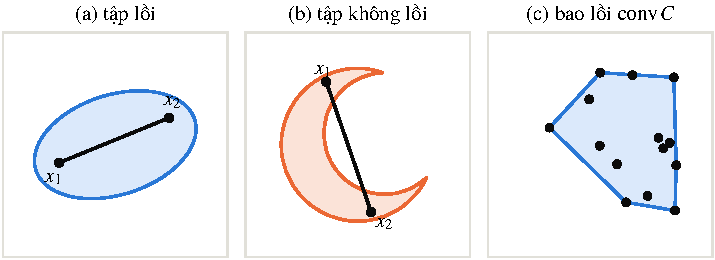
\includegraphics[width=\linewidth]{fig_convex_sets.pdf}
\caption[Tập lồi, tập không lồi và bao lồi]{(a) Một tập lồi: đoạn thẳng nối hai điểm bất kỳ nằm trọn trong tập. (b) Một tập không lồi. (c) Bao lồi của một tập hữu hạn điểm là đa giác lồi nhỏ nhất chứa các điểm đó.}
\label{fig:convex}
\end{figure}

\begin{example}\label{ex:convex-sets}
Một số tập lồi sẽ gặp lại nhiều lần trong đề án:
\begin{enumerate}[label=(\alph*),leftmargin=2em]
\item \emph{Siêu phẳng} $H=\{x:\ a^\T x=b\}$ với $a\in\R^n\setminus\{0\}$ và $b\in\R$. Đây là một tập affine; vectơ $a$ vuông góc với $H$ và được gọi là vectơ pháp tuyến của $H$.
\item \emph{Nửa không gian} $\{x:\ a^\T x\le b\}$ với $a\neq0$. Nếu $a^\T x_1\le b$ và $a^\T x_2\le b$ thì $a^\T\bigl(\theta x_1+(1-\theta)x_2\bigr)\le b$ với mọi $\theta\in[0,1]$, nên nửa không gian là tập lồi. Siêu phẳng $a^\T x=b$ chia $\R^n$ thành hai nửa không gian $\{a^\T x\le b\}$ và $\{a^\T x\ge b\}$; bộ phân loại tuyến tính chính là quy tắc xếp mỗi điểm vào một trong hai nửa không gian đó.
\item \emph{Hình cầu Euclid} $B(x_c,r)=\{x:\ \|x-x_c\|\le r\}$ với $r>0$. Nếu $x_1,x_2\in B(x_c,r)$ và $\theta\in[0,1]$ thì theo bất đẳng thức tam giác
\[
\|\theta x_1+(1-\theta)x_2-x_c\|\le\theta\|x_1-x_c\|+(1-\theta)\|x_2-x_c\|\le r,
\]
nên hình cầu là tập lồi.
\end{enumerate}
\end{example}

\begin{definition}\label{def:polyhedron}
\emph{Đa diện} là tập nghiệm của một hệ hữu hạn phương trình và bất phương trình tuyến tính:
\begin{equation}\label{eq:polyhedron}
P=\bigl\{x:\ a_j^\T x\le b_j,\ j=1,\dots,m;\ \ c_j^\T x=d_j,\ j=1,\dots,p\bigr\}.
\end{equation}
\end{definition}

Như vậy, đa diện là giao của hữu hạn nửa không gian và siêu phẳng (\cref{fig:separation}a). Không gian con, siêu phẳng, nửa không gian, đoạn thẳng và bao lồi của một tập hữu hạn điểm đều là đa diện. Một ví dụ quan trọng về sau: với dữ liệu $\{(x_k,y_k)\}$ cố định, tập các cặp $(w,w_0)\in\R^{n+1}$ thỏa mãn $y_k(w^\T x_k+w_0)\ge1$ với mọi $k$ là một đa diện trong không gian các tham số; đó là miền ràng buộc của bài toán SVM lề cứng ở Mục~\ref{sec:hardmargin}. Tính lồi của đa diện là hệ quả của mệnh đề sau.

\begin{proposition}\label{prop:convex-ops}
\begin{enumerate}[label=(\roman*),leftmargin=2em]
\item Giao của một họ tùy ý các tập lồi là tập lồi.
\item Nếu $f(x)=Ax+b$ là một ánh xạ affine từ $\R^n$ vào $\R^m$ và $S\subseteq\R^n$, $T\subseteq\R^m$ là các tập lồi, thì ảnh $f(S)=\{f(x):\ x\in S\}$ và nghịch ảnh $f^{-1}(T)=\{x:\ f(x)\in T\}$ là các tập lồi.
\end{enumerate}
\end{proposition}

\begin{proof}
(i) Nếu $x_1,x_2$ thuộc mọi tập trong họ thì đoạn $[x_1,x_2]$ cũng vậy. (ii) Ánh xạ affine bảo toàn tổ hợp lồi: $f\bigl(\theta x_1+(1-\theta)x_2\bigr)=\theta f(x_1)+(1-\theta)f(x_2)$. Do đó nếu $f(x_1),f(x_2)\in f(S)$ thì mọi điểm của đoạn nối chúng có dạng $f(\theta x_1+(1-\theta)x_2)\in f(S)$; lập luận tương tự cho nghịch ảnh.
\end{proof}

% ----------------------------------------------------------------------------
\section{Siêu phẳng phân tách và siêu phẳng tựa}\label{sec:separation}

Bài toán phân loại tuyến tính đặt ra một câu hỏi hình học: khi nào hai tập điểm có thể được tách bởi một siêu phẳng? Với các tập lồi, câu trả lời được cho bởi định lý siêu phẳng phân tách. Công cụ để chứng minh định lý là phép chiếu lên một tập lồi đóng.

\begin{lemma}[Phép chiếu lên tập lồi đóng]\label{lem:projection}
Cho $C\subseteq\R^n$ là tập lồi, đóng, khác rỗng và $x_0\in\R^n$. Khi đó tồn tại duy nhất một điểm $c^\ast\in C$ gần $x_0$ nhất, ký hiệu $c^\ast=\Pi_C(x_0)$. Hơn nữa, $c^\ast$ được đặc trưng bởi bất đẳng thức
\begin{equation}\label{eq:projection}
(x_0-c^\ast)^\T(x-c^\ast)\le0\qquad\text{với mọi } x\in C .
\end{equation}
\end{lemma}

\begin{proof}
\emph{Tồn tại.} Lấy một điểm $\bar c\in C$. Điểm gần nhất, nếu có, phải thuộc tập $C\cap B\bigl(x_0,\|x_0-\bar c\|\bigr)$; tập này compact và khác rỗng, nên hàm liên tục $x\mapsto\|x-x_0\|$ đạt cực tiểu trên nó.

\emph{Đặc trưng.} Với $x\in C$ và $t\in(0,1]$, điểm $c^\ast+t(x-c^\ast)$ thuộc $C$, nên
\[
0\le\|x_0-c^\ast-t(x-c^\ast)\|^2-\|x_0-c^\ast\|^2=-2t\,(x_0-c^\ast)^\T(x-c^\ast)+t^2\|x-c^\ast\|^2 .
\]
Chia cho $t$ rồi cho $t\to0^+$ ta được~\eqref{eq:projection}. Ngược lại, nếu $c^\ast\in C$ thỏa~\eqref{eq:projection} thì với mọi $x\in C$,
$\|x_0-x\|^2=\|x_0-c^\ast\|^2-2(x_0-c^\ast)^\T(x-c^\ast)+\|x-c^\ast\|^2\ge\|x_0-c^\ast\|^2$, dấu bằng chỉ khi $x=c^\ast$. Điều này đồng thời chứng minh tính duy nhất.
\end{proof}

\begin{theorem}[Siêu phẳng phân tách]\label{thm:separation}
Cho $C$ và $D$ là hai tập lồi, khác rỗng và rời nhau trong $\R^n$. Khi đó tồn tại $a\neq0$ và $b\in\R$ sao cho $a^\T x\le b$ với mọi $x\in C$ và $a^\T x\ge b$ với mọi $x\in D$. Nếu thêm giả thiết $C$ và $D$ đóng, trong đó ít nhất một tập compact, thì có thể chọn $a,b$ để phân tách là chặt:
\begin{equation}\label{eq:strict-sep}
a^\T x<b<a^\T z\qquad\text{với mọi } x\in C,\ z\in D .
\end{equation}
\end{theorem}

\begin{proof}
Ta chứng minh trường hợp phân tách chặt, là trường hợp sẽ được dùng; trường hợp tổng quát xem~\cite[Mục~2.5.1]{boyd2004}. Tập $E=D-C=\{z-x:\ x\in C,\ z\in D\}$ là tập lồi (theo \cref{prop:convex-ops}(ii), vì nó là ảnh của tập lồi $C\times D$ qua ánh xạ tuyến tính $(x,z)\mapsto z-x$), đóng (vì một trong hai tập compact) và không chứa $0$ (vì $C\cap D=\emptyset$). Đặt $u=\Pi_E(0)\neq0$. Theo~\eqref{eq:projection} với $x_0=0$, ta có $(0-u)^\T(e-u)\le0$, tức là $u^\T e\ge\|u\|^2$ với mọi $e\in E$. Nói cách khác, $u^\T z-u^\T x\ge\|u\|^2>0$ với mọi $x\in C$, $z\in D$. Chọn $a=u$ và $b=\sup_{x\in C}u^\T x+\tfrac12\|u\|^2$, ta được~\eqref{eq:strict-sep}.
\end{proof}

Trong chứng minh trên, $u=z^\ast-x^\ast$ với $x^\ast\in C$, $z^\ast\in D$ là cặp điểm gần nhau nhất của hai tập, và siêu phẳng tách có pháp tuyến cùng phương với đoạn nối cặp điểm đó (\cref{fig:separation}b). Hình ảnh này sẽ xuất hiện lại khi ta diễn giải bài toán đối ngẫu của SVM ở Mục~\ref{sec:hardmargin}.

\begin{theorem}[Siêu phẳng tựa]\label{thm:support}
Cho $C$ là tập lồi và $x_0$ là một điểm biên của $C$. Khi đó tồn tại $a\neq0$ sao cho $a^\T x\le a^\T x_0$ với mọi $x\in C$; siêu phẳng $\{x:\ a^\T x=a^\T x_0\}$ được gọi là siêu phẳng tựa của $C$ tại $x_0$.
\end{theorem}

Định lý được suy ra bằng cách áp dụng \cref{thm:separation} cho phần trong của $C$ và tập $\{x_0\}$ (khi phần trong khác rỗng), xem~\cite[Mục~2.5.2]{boyd2004}. Về mặt hình học, siêu phẳng tựa chạm vào $C$ tại $x_0$ và để toàn bộ $C$ về một phía (\cref{fig:separation}c).

\begin{figure}[t]
\centering
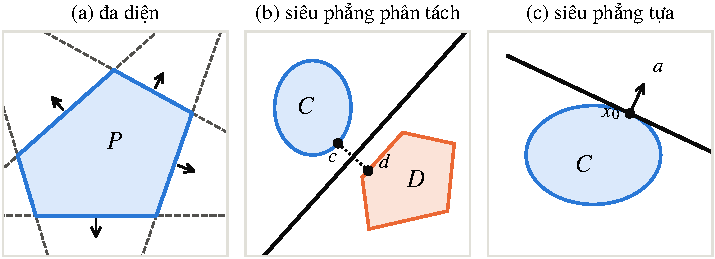
\includegraphics[width=\linewidth]{fig_separation.pdf}
\caption[Đa diện, siêu phẳng phân tách và siêu phẳng tựa]{(a) Đa diện $P$ là giao của năm nửa không gian; mũi tên chỉ vectơ pháp tuyến $a_j$ hướng ra ngoài. (b) Siêu phẳng phân tách hai tập lồi rời nhau $C$ và $D$, dựng từ cặp điểm gần nhau nhất $c\in C$, $d\in D$ như trong chứng minh \cref{thm:separation}. (c) Siêu phẳng tựa của tập lồi $C$ tại điểm biên $x_0$.}
\label{fig:separation}
\end{figure}

Hệ quả sau chuyển \cref{thm:separation} sang ngôn ngữ của dữ liệu và là cầu nối trực tiếp sang SVM lề cứng. Ta nói hai tập hữu hạn điểm $A$ và $B$ \emph{tách tuyến tính được} nếu tồn tại $(w,w_0)$ sao cho $w^\T x+w_0>0$ với mọi $x\in A$ và $w^\T x+w_0<0$ với mọi $x\in B$.

\begin{corollary}\label{cor:separable}
Cho dữ liệu $\{(x_k,y_k)\}_{k=1}^N$ với $y_k\in\{-1,+1\}$ và cả hai lớp đều khác rỗng; đặt $A=\{x_k:\ y_k=+1\}$, $B=\{x_k:\ y_k=-1\}$. Ba khẳng định sau là tương đương:
\begin{enumerate}[label=(\roman*),leftmargin=2em]
\item $A$ và $B$ tách tuyến tính được;
\item tồn tại $(w,w_0)$ sao cho $y_k(w^\T x_k+w_0)\ge1$ với mọi $k$;
\item $\conv A\cap\conv B=\emptyset$.
\end{enumerate}
\end{corollary}

\begin{proof}
(i)$\Rightarrow$(ii): đặt $\mu=\min_k y_k(w^\T x_k+w_0)>0$ và thay $(w,w_0)$ bởi $(w,w_0)/\mu$. (ii)$\Rightarrow$(iii): hai nửa không gian $\{x:\ w^\T x+w_0\ge1\}$ và $\{x:\ w^\T x+w_0\le-1\}$ là các tập lồi rời nhau, lần lượt chứa $A$ và $B$, nên cũng chứa $\conv A$ và $\conv B$; do đó hai bao lồi rời nhau. (iii)$\Rightarrow$(i): bao lồi của một tập hữu hạn là ảnh của đơn hình chuẩn (compact) qua một ánh xạ tuyến tính, nên compact; áp dụng phần phân tách chặt của \cref{thm:separation} cho $\conv A$ và $\conv B$ với $w=-a$, $w_0=b$.
\end{proof}

% ----------------------------------------------------------------------------
\section{Hàm lồi và bài toán tối ưu lồi}\label{sec:convexopt}

\begin{definition}\label{def:convex-fn}
Cho $C\subseteq\R^n$ là tập lồi. Hàm $f:C\to\R$ được gọi là \emph{hàm lồi} nếu
\[
f\bigl(\theta x+(1-\theta)z\bigr)\le\theta f(x)+(1-\theta)f(z)\qquad\text{với mọi } x,z\in C,\ \theta\in[0,1];
\]
$f$ được gọi là \emph{lồi chặt} nếu bất đẳng thức là chặt khi $x\neq z$ và $\theta\in(0,1)$. Hàm $f$ là \emph{lõm} nếu $-f$ lồi.
\end{definition}

Hàm affine vừa lồi vừa lõm. Mọi chuẩn là hàm lồi, theo bất đẳng thức tam giác; hàm $\|x\|^2$ lồi chặt. Hàm bản lề $t\mapsto\max\{0,t\}$ và hàm mất mát $t\mapsto\max\{0,1-t\}$ dùng trong SVM là hàm lồi. Ba phép toán sau cho phép kiểm tra tính lồi của các hàm mục tiêu trong đề án mà không cần tính toán trực tiếp.

\begin{proposition}\label{prop:convex-fn-ops}
\begin{enumerate}[label=(\roman*),leftmargin=2em]
\item Nếu $f_1,\dots,f_m$ lồi và $c_1,\dots,c_m\ge0$ thì $\sum_ic_if_i$ lồi; nếu thêm một $f_i$ lồi chặt với $c_i>0$ thì tổng lồi chặt.
\item Nếu $f_1,\dots,f_m$ lồi thì $x\mapsto\max_i f_i(x)$ lồi.
\item Nếu $f$ lồi thì $x\mapsto f(Ax+b)$ lồi.
\end{enumerate}
\end{proposition}

\begin{proof}
(i) và (iii) suy trực tiếp từ định nghĩa. Với (ii), với mỗi $i$ ta có $f_i\bigl(\theta x+(1-\theta)z\bigr)\le\theta f_i(x)+(1-\theta)f_i(z)\le\theta\max_jf_j(x)+(1-\theta)\max_jf_j(z)$; lấy cực đại theo $i$ ở vế trái.
\end{proof}

Chẳng hạn, với dữ liệu cố định, hàm $(w,w_0)\mapsto\frac12\|w\|^2+\gamma\sum_k\max\{0,\,1-y_k(w^\T x_k+w_0)\}$ là hàm lồi: mỗi số hạng $\max\{0,\,1-y_k(w^\T x_k+w_0)\}$ là cực đại của hai hàm affine theo $(w,w_0)$. Đây là hàm mục tiêu của SVM lề mềm (Mục~\ref{sec:softmargin}).

Đối với hàm khả vi, tính lồi có một đặc trưng hình học đơn giản: đồ thị nằm phía trên mọi tiếp diện. Cụ thể, nếu $C$ mở và $f$ khả vi trên $C$ thì $f$ lồi khi và chỉ khi
\begin{equation}\label{eq:first-order}
f(z)\ge f(x)+\nabla f(x)^\T(z-x)\qquad\text{với mọi } x,z\in C
\end{equation}
\cite[Mục~3.1.3]{boyd2004}. Hệ quả trực tiếp: nếu $\nabla f(x^\ast)=0$ thì $x^\ast$ là điểm cực tiểu toàn cục của $f$ trên $C$.

\paragraph{Bài toán tối ưu lồi.} Ta xét bài toán dạng chuẩn
\begin{equation}\label{eq:convex-problem}
\begin{aligned}
\min_{x}\quad & f_0(x)\\
\text{với điều kiện}\quad & f_i(x)\le0,\ \ i=1,\dots,m;\qquad h_j(x)=0,\ \ j=1,\dots,p,
\end{aligned}
\end{equation}
trong đó $f_0,\dots,f_m$ là các hàm lồi và $h_j(x)=g_j^\T x-e_j$ là các hàm affine. Theo \cref{prop:convex-ops}, tập chấp nhận được của~\eqref{eq:convex-problem} là tập lồi. Giá trị tối ưu được ký hiệu là $p^\ast$.

\begin{theorem}\label{thm:local-global}
Đối với bài toán~\eqref{eq:convex-problem}, mọi điểm cực tiểu địa phương đều là điểm cực tiểu toàn cục. Nếu $f_0$ lồi chặt thì bài toán có không quá một nghiệm.
\end{theorem}

\begin{proof}
Giả sử $x$ là cực tiểu địa phương nhưng có điểm chấp nhận được $z$ với $f_0(z)<f_0(x)$. Với $\theta\in(0,1]$, điểm $x_\theta=(1-\theta)x+\theta z$ chấp nhận được và $f_0(x_\theta)\le(1-\theta)f_0(x)+\theta f_0(z)<f_0(x)$. Khi $\theta\to0$, $x_\theta$ tiến tới $x$, mâu thuẫn với tính cực tiểu địa phương. Nếu $x\neq z$ là hai nghiệm và $f_0$ lồi chặt thì trung điểm của chúng chấp nhận được và có giá trị mục tiêu nhỏ hơn $p^\ast$, vô lý.
\end{proof}

Ba lớp bài toán lồi sẽ xuất hiện trong đề án. \emph{Quy hoạch tuyến tính}: $f_0$ và mọi $f_i$ đều affine. \emph{Quy hoạch toàn phương}: $f_0(x)=\frac12x^\T Qx+c^\T x$ với $Q$ nửa xác định dương và các ràng buộc affine; bài toán gốc và bài toán đối ngẫu của SVM thuộc lớp này. \emph{Bình phương tối thiểu có chính quy hóa}: $\min_x\|Ax-t\|^2+\lambda\|x\|^2$ với $\lambda>0$; hàm mục tiêu lồi chặt, và cho gradient bằng $0$ ta được nghiệm duy nhất $x^\ast=(A^\T A+\lambda I)^{-1}A^\T t$. Lớp thứ ba là dạng của LS-SVM và của hồi quy ridge (Mục~\ref{sec:pwlsvm}).

% ----------------------------------------------------------------------------
\section{Đối ngẫu Lagrange và điều kiện KKT}\label{sec:duality}

Lý thuyết đối ngẫu gắn với mỗi bài toán tối ưu có ràng buộc một bài toán khác, gọi là bài toán đối ngẫu, mà nghiệm của nó cho một cận dưới của giá trị tối ưu. Với SVM, bài toán đối ngẫu có cấu trúc đặc biệt: nó chỉ phụ thuộc vào dữ liệu qua các tích vô hướng, điều dẫn tới thủ thuật hạt nhân ở Mục~\ref{sec:kernel}.

\begin{definition}\label{def:lagrangian}
\emph{Hàm Lagrange} của bài toán~\eqref{eq:convex-problem} là
\[
L(x,\lambda,\nu)=f_0(x)+\sum_{i=1}^{m}\lambda_if_i(x)+\sum_{j=1}^{p}\nu_jh_j(x),\qquad\lambda\in\R^m,\ \nu\in\R^p;
\]
$\lambda_i,\nu_j$ được gọi là các \emph{nhân tử Lagrange}. \emph{Hàm đối ngẫu} là $g(\lambda,\nu)=\inf_xL(x,\lambda,\nu)$, và \emph{bài toán đối ngẫu} là $\max\,g(\lambda,\nu)$ với điều kiện $\lambda\ge0$; giá trị tối ưu của nó được ký hiệu là $d^\ast$.
\end{definition}

Vì $g$ là cận dưới đúng của một họ hàm affine theo $(\lambda,\nu)$, hàm đối ngẫu luôn lõm, và bài toán đối ngẫu luôn là một bài toán lồi, bất kể bài toán gốc có lồi hay không.

\begin{proposition}[Đối ngẫu yếu]\label{prop:weak-duality}
Với mọi $\lambda\ge0$ và mọi $\nu$, ta có $g(\lambda,\nu)\le p^\ast$. Do đó $d^\ast\le p^\ast$.
\end{proposition}

\begin{proof}
Nếu $\tilde x$ chấp nhận được thì $\lambda_if_i(\tilde x)\le0$ và $h_j(\tilde x)=0$, nên $g(\lambda,\nu)\le L(\tilde x,\lambda,\nu)\le f_0(\tilde x)$. Lấy cận dưới đúng theo mọi $\tilde x$ chấp nhận được ta được $g(\lambda,\nu)\le p^\ast$.
\end{proof}

Hiệu $p^\ast-d^\ast\ge0$ được gọi là \emph{khoảng cách đối ngẫu}. Khi $p^\ast=d^\ast$, ta nói có \emph{đối ngẫu mạnh}. Đối với bài toán lồi, đối ngẫu mạnh xảy ra dưới những điều kiện khá nhẹ; điều kiện thông dụng nhất như sau.

\begin{theorem}[Điều kiện Slater~{\cite[Mục~5.2.3]{boyd2004}}]\label{thm:slater}
Giả sử bài toán~\eqref{eq:convex-problem} là lồi và có một điểm chấp nhận được $x$ sao cho $f_i(x)<0$ với mọi $i$ mà $f_i$ không phải là hàm affine. Khi đó $d^\ast=p^\ast$, và nếu $p^\ast>-\infty$ thì bài toán đối ngẫu có nghiệm.
\end{theorem}

Đặc biệt, khi mọi ràng buộc đều affine, như trong các bài toán SVM, chỉ cần bài toán gốc có điểm chấp nhận được là có đối ngẫu mạnh. Khi có đối ngẫu mạnh, nghiệm của hai bài toán liên hệ với nhau qua hệ điều kiện sau.

\begin{definition}[Điều kiện KKT]\label{def:kkt}
Giả sử $f_0,f_i,h_j$ khả vi. Bộ $(x,\lambda,\nu)$ thỏa mãn \emph{điều kiện Karush--Kuhn--Tucker} nếu
\begin{enumerate}[label=(\alph*),leftmargin=2em]
\item $f_i(x)\le0$ và $h_j(x)=0$ với mọi $i,j$ (chấp nhận được đối với bài toán gốc);
\item $\lambda\ge0$ (chấp nhận được đối với bài toán đối ngẫu);
\item $\lambda_if_i(x)=0$ với mọi $i$ (điều kiện bù);
\item $\nabla f_0(x)+\sum_i\lambda_i\nabla f_i(x)+\sum_j\nu_j\nabla h_j(x)=0$ (điều kiện dừng).
\end{enumerate}
\end{definition}

\begin{theorem}\label{thm:kkt}
\begin{enumerate}[label=(\roman*),leftmargin=2em]
\item Nếu có đối ngẫu mạnh, $x^\ast$ là nghiệm của bài toán gốc và $(\lambda^\ast,\nu^\ast)$ là nghiệm của bài toán đối ngẫu, thì $(x^\ast,\lambda^\ast,\nu^\ast)$ thỏa mãn điều kiện KKT.
\item Ngược lại, nếu bài toán lồi và $(\tilde x,\tilde\lambda,\tilde\nu)$ thỏa mãn điều kiện KKT, thì $\tilde x$ và $(\tilde\lambda,\tilde\nu)$ lần lượt là nghiệm của bài toán gốc và bài toán đối ngẫu, và khoảng cách đối ngẫu bằng $0$.
\end{enumerate}
\end{theorem}

\begin{proof}
Ta chứng minh (ii); chứng minh (i) xem~\cite[Mục~5.5.3]{boyd2004}. Vì $\tilde\lambda\ge0$, hàm $x\mapsto L(x,\tilde\lambda,\tilde\nu)$ lồi, và theo (d) gradient của nó bằng $0$ tại $\tilde x$; do~\eqref{eq:first-order}, $\tilde x$ là điểm cực tiểu toàn cục của nó. Vậy
\[
g(\tilde\lambda,\tilde\nu)=L(\tilde x,\tilde\lambda,\tilde\nu)=f_0(\tilde x)+\sum_i\tilde\lambda_if_i(\tilde x)+\sum_j\tilde\nu_jh_j(\tilde x)=f_0(\tilde x),
\]
trong đó đẳng thức cuối dùng (a) và (c). Theo \cref{prop:weak-duality}, $f_0(\tilde x)=g(\tilde\lambda,\tilde\nu)\le d^\ast\le p^\ast\le f_0(\tilde x)$, nên mọi bất đẳng thức đều là đẳng thức.
\end{proof}

Điều kiện bù (c) có một ý nghĩa sẽ được dùng nhiều lần: nếu $\lambda_i^\ast>0$ thì ràng buộc thứ $i$ phải \emph{chặt}, $f_i(x^\ast)=0$. Trong SVM, điều này có nghĩa là chỉ những điểm dữ liệu nằm đúng trên lề mới có nhân tử dương; đó là các vectơ hỗ trợ. Hai ví dụ dưới đây minh họa lý thuyết trên những bài toán nhỏ mà ta sẽ gặp lại.

\begin{example}[Khoảng cách từ một điểm đến một siêu phẳng]\label{ex:distance}
Cho siêu phẳng $H=\{x:\ w^\T x+b=0\}$ với $w\neq0$ và một điểm $x_0$. Xét bài toán $\min\ \frac12\|x-x_0\|^2$ với điều kiện $w^\T x+b=0$. Hàm Lagrange là $\frac12\|x-x_0\|^2+\nu(w^\T x+b)$; điều kiện dừng cho $x=x_0-\nu w$, và thay vào ràng buộc ta được $\nu=(w^\T x_0+b)/\|w\|^2$. Vì bài toán lồi, theo \cref{thm:kkt}(ii) nghiệm là
\[
x^\ast=x_0-\frac{w^\T x_0+b}{\|w\|^2}\,w,\qquad\text{và}\qquad \operatorname{dist}(x_0,H)=\|x_0-x^\ast\|=\frac{|w^\T x_0+b|}{\|w\|}.
\]
Công thức này (\cref{fig:duality}a) là cơ sở của khái niệm lề trong SVM.
\end{example}

\begin{example}[Một bài toán đối ngẫu tường minh]\label{ex:dual-toy}
Xét bài toán $\min\ x^2$ với điều kiện $1-x\le0$, có nghiệm $x^\ast=1$ và $p^\ast=1$. Hàm Lagrange $L(x,\lambda)=x^2+\lambda(1-x)$ đạt cực tiểu theo $x$ tại $x=\lambda/2$, nên $g(\lambda)=\lambda-\lambda^2/4$. Bài toán đối ngẫu $\max_{\lambda\ge0}g(\lambda)$ có nghiệm $\lambda^\ast=2$ và $d^\ast=1=p^\ast$ (\cref{fig:duality}b). Điều kiện bù $\lambda^\ast(1-x^\ast)=0$ thỏa mãn vì ràng buộc chặt tại nghiệm.
\end{example}

\begin{figure}[t]
\centering
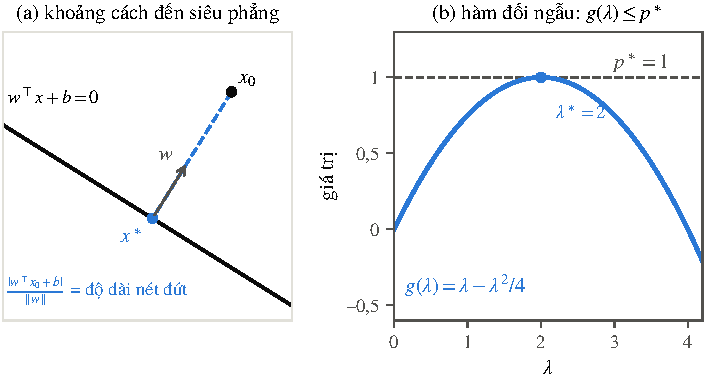
\includegraphics[width=\linewidth]{fig_duality.pdf}
\caption[Khoảng cách đến siêu phẳng và đối ngẫu yếu]{(a) Hình chiếu $x^\ast$ của điểm $x_0$ lên siêu phẳng $w^\T x+b=0$ (\cref{ex:distance}). (b) Hàm đối ngẫu của \cref{ex:dual-toy} luôn nằm dưới giá trị tối ưu $p^\ast$ và chạm tới $p^\ast$ tại $\lambda^\ast=2$.}
\label{fig:duality}
\end{figure}

% ----------------------------------------------------------------------------
\section{Hàm tuyến tính từng phần liên tục}\label{sec:pwl-functions}

Hàm affine $\ell(x)=a^\T x+b$ là loại hàm đơn giản nhất: đồ thị của nó là một siêu phẳng trong $\R^{n+1}$. Bước mở rộng tự nhiên tiếp theo là chia miền xác định thành hữu hạn vùng đa diện và cho phép hàm là affine trên từng vùng, với điều kiện các mảnh được “dán” liền với nhau dọc theo biên chung. Lớp hàm thu được đủ phong phú để xấp xỉ mọi hàm liên tục trên một tập compact, nhưng vẫn giữ được phần lớn sự đơn giản của hàm affine. Đây là đối tượng trung tâm của đề án: biên quyết định của các mô hình PWL-SVM ở Chương~\ref{chap:2} chính là tập không điểm của những hàm như vậy.

\subsection{Định nghĩa và ví dụ}

\begin{definition}[Phân hoạch đa diện]\label{def:partition}
Cho $\Omega\subseteq\R^n$. Họ hữu hạn các đa diện $\{\Omega_1,\dots,\Omega_K\}$ được gọi là một \emph{phân hoạch đa diện} của $\Omega$ nếu
\[
\Omega=\bigcup_{k=1}^{K}\Omega_k \qquad\text{và}\qquad \intr\Omega_k\cap\intr\Omega_l=\emptyset\quad\text{với mọi } k\neq l .
\]
\end{definition}

Các vùng của một phân hoạch có thể có chung biên, nhưng phần trong của chúng không giao nhau. Chẳng hạn, ba dải ngang $\{x:\,0\le x(2)\le \tfrac13\}$, $\{x:\,\tfrac13\le x(2)\le\tfrac23\}$ và $\{x:\,\tfrac23\le x(2)\le 1\}$ của hình vuông đơn vị ở \cref{fig:moons} là một phân hoạch đa diện của hình vuông đó.

\begin{definition}[Hàm tuyến tính từng phần liên tục]\label{def:pwl-function}
Hàm $f:\Omega\to\R$ được gọi là \emph{hàm tuyến tính từng phần liên tục}, gọi tắt là \emph{hàm PWL}, nếu $f$ liên tục trên $\Omega$ và tồn tại một phân hoạch đa diện $\{\Omega_1,\dots,\Omega_K\}$ của $\Omega$ cùng các hàm affine $\ell_k(x)=a_k^\T x+b_k$ sao cho
\begin{equation}\label{eq:pwl-def}
f(x)=\ell_k(x)\qquad\text{với mọi } x\in\Omega_k,\quad k=1,\dots,K.
\end{equation}
Các hàm $\ell_1,\dots,\ell_K$ được gọi là các \emph{mảnh} (hay các hàm affine cục bộ) của $f$.
\end{definition}

\begin{remark}\label{rem:terminology}
Theo nghĩa chặt, các hàm trong \cref{def:pwl-function} nên gọi là \emph{affine} từng phần, vì mỗi mảnh là một hàm affine chứ không nhất thiết là hàm tuyến tính. Đề án dùng thuật ngữ “tuyến tính từng phần” theo thói quen trong tài liệu học máy và theo bài báo gốc~\cite{huang2013}. Điều kiện liên tục là thiết yếu: một hàm bậc thang cũng bằng hằng số trên từng mảnh nhưng không thuộc lớp hàm đang xét. Trong toàn bộ đề án, “hàm PWL” luôn được hiểu là hàm tuyến tính từng phần \emph{liên tục}.
\end{remark}

\begin{example}\label{ex:pwl}
Một số hàm PWL sẽ gặp lại nhiều lần trong đề án:
\begin{enumerate}[label=(\alph*),leftmargin=2em]
\item Hàm giá trị tuyệt đối $|t|=\max\{t,-t\}$ là hàm PWL trên $\R$ với hai mảnh: $-t$ trên $(-\infty,0]$ và $t$ trên $[0,+\infty)$.
\item Hàm bản lề $h(t)=\max\{0,t\}$, ký hiệu $(t)_+$, có hai mảnh là $0$ và $t$ (\cref{fig:hinge1d}a). Trong mạng nơ-ron, hàm này được gọi là hàm kích hoạt ReLU.
\item Với $p\in\R^n\setminus\{0\}$ và $q\in\R$, hàm $x\mapsto\max\{0,\,p^\T x+q\}$ là hàm PWL trên $\R^n$ với hai mảnh, ngăn cách bởi siêu phẳng $p^\T x+q=0$. Đồ thị của nó gồm hai nửa siêu phẳng nối với nhau dọc theo một “bản lề”; vì thế Breiman~\cite{breiman1993} gọi nó là \emph{siêu phẳng bản lề} (hinging hyperplane).
\item Hàm hai biến
\[
\begin{aligned}
f(x)={}&0{,}15+0{,}25\,x(1)+0{,}2\,x(2)+0{,}9\,\bigl(x(1)+x(2)-0{,}9\bigr)_+\\
&-1{,}2\,\bigl(x(1)-0{,}6\bigr)_+ +0{,}8\,\bigl(0{,}45-x(2)\bigr)_+
\end{aligned}
\]
trên hình vuông đơn vị có bảy mảnh (\cref{fig:pwlsurface}). Ba đường thẳng mà tại đó các số hạng bản lề đổi trạng thái chia hình vuông thành bảy đa giác lồi $\Omega_1,\dots,\Omega_7$; trên mỗi đa giác, $f$ là một hàm affine và đồ thị của $f$ là một mảnh mặt phẳng.
\end{enumerate}
\end{example}

\begin{figure}[t]
\centering
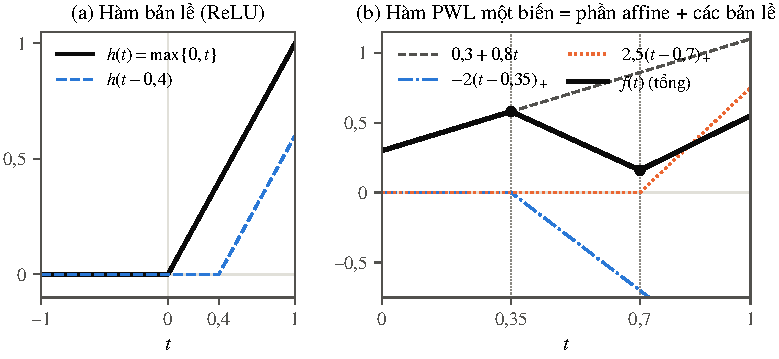
\includegraphics[width=\linewidth]{fig_hinge_1d.pdf}
\caption[Hàm bản lề và biểu diễn một hàm PWL một biến bằng các hàm bản lề]{(a) Hàm bản lề $h(t)=\max\{0,t\}$ và bản dịch chuyển của nó. (b) Hàm PWL một biến $f(t)=0{,}3+0{,}8t-2(t-0{,}35)_+ +2{,}5(t-0{,}7)_+$ là tổng của một hàm affine và hai hàm bản lề đặt tại hai điểm gãy; hệ số của mỗi bản lề bằng độ thay đổi hệ số góc tại điểm gãy đó (\cref{prop:1d}).}
\label{fig:hinge1d}
\end{figure}

\begin{figure}[t]
\centering
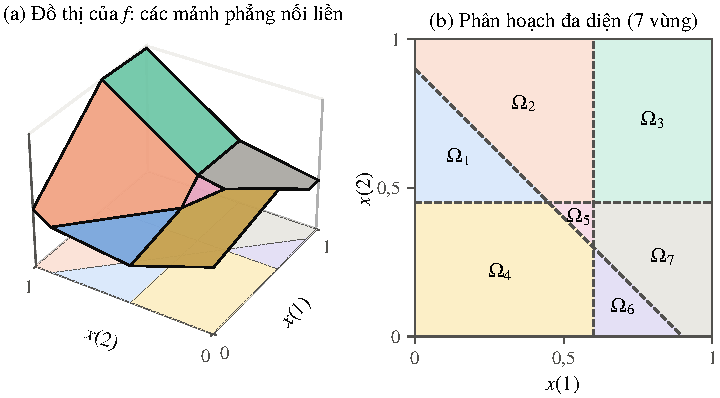
\includegraphics[width=\linewidth]{fig_pwl_surface.pdf}
\caption[Một hàm PWL hai biến và phân hoạch đa diện tương ứng]{Hàm PWL hai biến của \cref{ex:pwl}(d). (a) Đồ thị gồm bảy mảnh mặt phẳng nối liền nhau; các nếp gấp nằm trên ba đường thẳng $x(1)+x(2)=0{,}9$, $x(1)=0{,}6$ và $x(2)=0{,}45$. (b) Phân hoạch đa diện tương ứng của hình vuông đơn vị.}
\label{fig:pwlsurface}
\end{figure}

\subsection{Các phép toán bảo toàn tính tuyến tính từng phần}

Kiểm tra trực tiếp một hàm có phải là hàm PWL hay không theo \cref{def:pwl-function} thường khá phiền, vì phải chỉ ra được phân hoạch. Mệnh đề sau cho phép tạo ra các hàm PWL phức tạp từ những hàm đơn giản; nó sẽ được dùng nhiều lần ở Chương~\ref{chap:2}.

\begin{proposition}\label{prop:closure}
Giả sử $f,g:\R^n\to\R$ là các hàm PWL và $\alpha,\beta\in\R$. Khi đó $\alpha f+\beta g$, $\max\{f,g\}$ và $\min\{f,g\}$ đều là hàm PWL. Do đó, mọi hàm nhận được từ hữu hạn hàm affine bằng hữu hạn lần áp dụng các phép cộng, nhân với hằng số, lấy $\max$, lấy $\min$ và lấy trị tuyệt đối đều là hàm PWL.
\end{proposition}

\begin{proof}
Gọi $\{P_i\}_{i=1}^{I}$ và $\{Q_j\}_{j=1}^{J}$ là các phân hoạch đa diện của $\R^n$ ứng với $f$ và $g$, với các mảnh tương ứng là $\ell_i$ và $m_j$. Mỗi tập $R_{ij}=P_i\cap Q_j$ là một đa diện, vì là giao của hữu hạn nửa không gian. Họ $\{R_{ij}\}$ phủ $\R^n$ và có phần trong đôi một rời nhau: nếu $(i,j)\neq(i',j')$ thì hoặc $\intr P_i\cap\intr P_{i'}=\emptyset$, hoặc $\intr Q_j\cap\intr Q_{j'}=\emptyset$. Trên $R_{ij}$ ta có $\alpha f+\beta g=\alpha\ell_i+\beta m_j$ là hàm affine; hơn nữa $\alpha f+\beta g$ liên tục. Vậy $\alpha f+\beta g$ là hàm PWL.

Với $\max\{f,g\}$, ta chia tiếp mỗi $R_{ij}$ thành hai đa diện
\[
R_{ij}^{+}=R_{ij}\cap\{x:\ \ell_i(x)\ge m_j(x)\},\qquad R_{ij}^{-}=R_{ij}\cap\{x:\ \ell_i(x)\le m_j(x)\}
\]
(nếu $\ell_i\equiv m_j$ thì giữ nguyên $R_{ij}$). Khi $\ell_i-m_j$ không đồng nhất bằng hằng số, hai nửa không gian đóng $\{\ell_i\ge m_j\}$ và $\{\ell_i\le m_j\}$ có phần trong rời nhau; khi $\ell_i-m_j$ là hằng số khác $0$, một trong hai tập là rỗng. Vì vậy họ các tập $R_{ij}^{\pm}$ vẫn là một phân hoạch đa diện của $\R^n$, và trên $R_{ij}^{+}$ (tương ứng $R_{ij}^{-}$) ta có $\max\{f,g\}=\ell_i$ (tương ứng $m_j$). Hàm $\max\{f,g\}$ liên tục vì là cực đại của hai hàm liên tục, nên nó là hàm PWL. Trường hợp $\min\{f,g\}=-\max\{-f,-g\}$ suy ra từ hai trường hợp trên.

Khẳng định cuối có được bằng quy nạp, vì mỗi hàm affine là hàm PWL với phân hoạch tầm thường $\{\R^n\}$ và $|f|=\max\{f,-f\}$.
\end{proof}

\begin{corollary}\label{cor:forms}
Các hàm có dạng $\max\limits_{1\le j\le J}\ \min\limits_{i\in S_j}\ \ell_i(x)$, với $\ell_i$ affine và $S_j$ là các tập chỉ số hữu hạn, cũng như các hàm có dạng tổng các bản lề
\[
a^\T x+b+\sum_{m=1}^{D} c_m\max\{0,\,p_m^\T x+q_m\},
\]
đều là hàm PWL trên $\R^n$.
\end{corollary}

\subsection{Hàm tuyến tính từng phần một biến}

Khi $n=1$, cấu trúc của hàm PWL đặc biệt đơn giản: phân hoạch của $\R$ gồm các khoảng nối tiếp nhau, ngăn cách bởi các \emph{điểm gãy}. Mệnh đề sau cho thấy mọi hàm như vậy là tổng của một hàm affine và các hàm bản lề đặt tại các điểm gãy.

\begin{proposition}\label{prop:1d}
Cho $f:\R\to\R$ là hàm PWL với các điểm gãy $t_1<t_2<\dots<t_K$, và gọi $s_0,s_1,\dots,s_K$ lần lượt là hệ số góc của $f$ trên các khoảng $(-\infty,t_1]$, $[t_1,t_2]$, \dots, $[t_K,+\infty)$. Khi đó, với mọi $t\in\R$,
\begin{equation}\label{eq:1d-hinge}
f(t)=f(t_1)+s_0\,(t-t_1)+\sum_{j=1}^{K}(s_j-s_{j-1})\,(t-t_j)_+ .
\end{equation}
\end{proposition}

\begin{proof}
Ký hiệu $g(t)$ là vế phải của~\eqref{eq:1d-hinge}. Trên $(-\infty,t_1]$ mọi số hạng bản lề đều bằng $0$, nên $g(t)=f(t_1)+s_0(t-t_1)=f(t)$, vì trên khoảng này $f$ là hàm affine với hệ số góc $s_0$. Giả sử $f=g$ trên $(-\infty,t_i]$ với một $i\in\{1,\dots,K\}$, và quy ước $t_{K+1}=+\infty$. Trên $[t_i,t_{i+1}]$, các số hạng bản lề với $j\le i$ bằng $t-t_j$, còn các số hạng với $j>i$ bằng $0$. Do đó $g$ là hàm affine trên khoảng này với hệ số góc
\[
s_0+\sum_{j=1}^{i}(s_j-s_{j-1})=s_i ,
\]
trùng với hệ số góc của $f$. Hai hàm affine có cùng hệ số góc và cùng giá trị tại $t_i$ thì trùng nhau, nên $f=g$ trên $(-\infty,t_{i+1}]$. Theo quy nạp, $f=g$ trên toàn $\R$.
\end{proof}

\begin{remark}\label{rem:1d}
Hệ số của hàm bản lề đặt tại $t_j$ chính là độ thay đổi hệ số góc $s_j-s_{j-1}$, tức là “độ gãy” của đồ thị tại $t_j$ (\cref{fig:hinge1d}b). Mệnh đề~\ref{prop:1d} có một hệ quả quan trọng cho học máy: nếu các điểm gãy được cố định trước, thì mọi hàm PWL một biến với các điểm gãy đó là tổ hợp tuyến tính của $K+2$ hàm \emph{cố định} $1,\ t,\ (t-t_1)_+,\dots,(t-t_K)_+$. Khi ấy, học một hàm PWL chỉ còn là tìm các hệ số của một tổ hợp tuyến tính, tức là một bài toán tuyến tính theo tham số. Đây chính là ý tưởng của ánh xạ đặc trưng cộng tính ở Mục~\ref{sec:maps}.
\end{remark}

\subsection{Biểu diễn hàm tuyến tính từng phần nhiều biến}

Khi $n\ge 2$, phân hoạch đa diện có thể rất phức tạp và các vùng không còn được sắp thứ tự tự nhiên như trên đường thẳng. Dù vậy, hai định lý dưới đây khẳng định rằng mọi hàm PWL vẫn viết được dưới những dạng tường minh và gọn. Chứng minh của chúng khá dài và nằm ngoài phạm vi đề án; ta chỉ phát biểu và phân tích ý nghĩa.

\begin{theorem}[Biểu diễn max--min~\cite{tarela1999,ovchinnikov2002}]\label{thm:lattice}
Cho $f:\R^n\to\R$ là hàm PWL với các mảnh $\ell_1,\dots,\ell_K$. Khi đó tồn tại các tập chỉ số $S_1,\dots,S_J\subseteq\{1,\dots,K\}$ sao cho
\begin{equation}\label{eq:lattice}
f(x)=\max_{1\le j\le J}\ \min_{i\in S_j}\ \ell_i(x)\qquad\text{với mọi } x\in\R^n .
\end{equation}
\end{theorem}

\begin{theorem}[Wang và Sun~{\cite[Định lý 1]{wang2005}}]\label{thm:wangsun}
Với mọi hàm PWL $f:\R^n\to\R$, tồn tại số nguyên dương $D$, các dấu $\sigma_1,\dots,\sigma_D\in\{-1,1\}$ và các hàm affine $\ell_{m,i}$ ($m=1,\dots,D$; $i=0,\dots,n$) sao cho
\begin{equation}\label{eq:ghh}
f(x)=\sum_{m=1}^{D}\sigma_m\max\bigl\{\ell_{m,0}(x),\,\ell_{m,1}(x),\dots,\ell_{m,n}(x)\bigr\}\qquad\text{với mọi } x\in\R^n .
\end{equation}
\end{theorem}

\begin{remark}\label{rem:ghh}
Có bốn điểm cần lưu ý về hai định lý trên.
\begin{enumerate}[label=(\roman*),leftmargin=2em]
\item Trong~\cite{wang2005}, mỗi số hạng là cực đại của \emph{không quá} $n+1$ hàm affine; lặp lại một hàm nếu cần, ta luôn có thể coi mỗi số hạng có đúng $n+1$ hàm như trong~\eqref{eq:ghh}. Mỗi số hạng là một dạng tổng quát của siêu phẳng bản lề, và Wang cùng Sun gọi mô hình~\eqref{eq:ghh} là \emph{siêu phẳng bản lề tổng quát} (GHH).
\item Khi $n=1$, mỗi số hạng $\max\{\ell_0,\ell_1\}=\ell_0+(\ell_1-\ell_0)_+$ là một hàm affine cộng một hàm bản lề, và~\eqref{eq:ghh} trở về dạng của \cref{prop:1d}. Khi $n\ge 2$, các số hạng hai mảnh $\max\{\ell_0,\ell_1\}$ của Breiman không còn đủ: tổng các siêu phẳng bản lề xấp xỉ được mọi hàm liên tục trên một tập compact~\cite{breiman1993} nhưng không biểu diễn đúng được mọi hàm PWL~\cite{wang2005}. \Cref{thm:wangsun} cho biết $n+1$ mảnh trong mỗi số hạng là đủ.
\item Cả hai định lý chỉ khẳng định sự tồn tại; số số hạng $J$ hay $D$ có thể lớn hơn nhiều so với số mảnh $K$. Trong thực hành, điều này trở thành câu hỏi: cần bao nhiêu đặc trưng? Chương~\ref{chap:3} sẽ trả lời câu hỏi này bằng thực nghiệm.
\item Lớp hàm PWL cũng chính là lớp hàm mà mạng nơ-ron ReLU biểu diễn được: một hàm $\R^n\to\R$ biểu diễn được bởi một mạng ReLU (với số lớp đủ lớn) khi và chỉ khi nó là hàm PWL~\cite{arora2018}.
\end{enumerate}
\end{remark}

% ----------------------------------------------------------------------------
% ----------------------------------------------------------------------------
\section*{Tiểu kết Chương 1}
\phantomsection\addcontentsline{toc}{section}{Tiểu kết Chương 1}

Chương 1 đã chuẩn bị ba nhóm công cụ. Thứ nhất là hình học lồi: tập lồi, đa diện và định lý siêu phẳng phân tách, trong đó \cref{cor:separable} cho điều kiện cần và đủ để hai tập điểm tách tuyến tính được. Thứ hai là tối ưu lồi và đối ngẫu: mọi cực tiểu địa phương của bài toán lồi là toàn cục, và khi các ràng buộc là affine, đối ngẫu mạnh cùng điều kiện KKT cho phép chuyển qua lại giữa bài toán gốc và bài toán đối ngẫu. Thứ ba là lớp hàm tuyến tính từng phần liên tục: lớp này đóng với các phép cộng, lấy cực đại và cực tiểu, và mọi hàm trong lớp đều viết được thành tổng các hàm bản lề tổng quát (\cref{thm:wangsun}). Chương~\ref{chap:2} dùng hai nhóm công cụ đầu để xây dựng SVM, và nhóm thứ ba để xây dựng ánh xạ đặc trưng tuyến tính từng phần.

% ============================================================================
%  CHƯƠNG 2. SVM VÀ SVM VỚI ÁNH XẠ ĐẶC TRƯNG TUYẾN TÍNH TỪNG PHẦN
% ============================================================================
\chapter{SVM và SVM với ánh xạ đặc trưng tuyến tính từng phần}\label{chap:2}

Đây là chương chính của đề án. \Cref{sec:hardmargin,sec:softmargin,sec:kernel} trình bày SVM theo trình tự lề cứng, lề mềm, ánh xạ đặc trưng và LS-SVM, dựa trên các công cụ tối ưu của Chương~\ref{chap:1}. \Cref{sec:pwlset,sec:pwlsvm,sec:maps} trình bày phương pháp của Huang, Mehrkanoon và Suykens~\cite{huang2013}: từ khái niệm tập tuyến tính từng phần, qua ánh xạ đặc trưng tuyến tính từng phần và các mô hình PWL-SVM, đến các dạng ánh xạ cụ thể và cách chọn tham số. \Cref{sec:relations} chỉ ra rằng một số bộ phân loại tuyến tính từng phần quen thuộc là trường hợp riêng của PWL-SVM.

Trong suốt chương, dữ liệu huấn luyện là $\{(x_k,y_k)\}_{k=1}^{N}$ với $x_k\in\R^n$ và nhãn $y_k\in\{-1,+1\}$; $x(i)$ là thành phần thứ $i$ của vectơ $x$. Một bộ phân loại là một hàm $f:\R^n\to\R$ cùng quy tắc gán nhãn $\hat y(x)=\sgn f(x)$; tập $\{x:\ f(x)=0\}$ là \emph{biên quyết định}. Ta luôn giả thiết cả hai lớp đều có mặt trong dữ liệu.

% ----------------------------------------------------------------------------
\section{Bài toán phân loại nhị phân và SVM lề cứng}\label{sec:hardmargin}

Bộ phân loại tuyến tính có dạng $f(x)=w^\T x+w_0$ với $w\in\R^n$ và hệ số chặn $w_0\in\R$; biên quyết định của nó là siêu phẳng $H=\{x:\ w^\T x+w_0=0\}$. Giả sử trước hết dữ liệu tách tuyến tính được. Khi đó thường có vô số siêu phẳng phân loại đúng toàn bộ dữ liệu huấn luyện (\cref{fig:hardmargin}a), và câu hỏi đặt ra là nên chọn siêu phẳng nào. Ý tưởng của SVM~\cite{cortes1995,vapnik1998} là chọn siêu phẳng cách xa dữ liệu nhất: một biên nằm sát một điểm huấn luyện sẽ dễ phân loại sai những điểm mới ở gần điểm đó, còn một biên có khoảng trống rộng hai bên thì chịu được các nhiễu loạn nhỏ của dữ liệu.

\paragraph{Lề và bài toán tối ưu.} Theo \cref{ex:distance}, khoảng cách từ $x_k$ đến $H$ là $|w^\T x_k+w_0|/\|w\|$. Nếu $H$ phân loại đúng $x_k$ thì $y_k(w^\T x_k+w_0)>0$, nên khoảng cách này bằng $y_k(w^\T x_k+w_0)/\|w\|$. \emph{Lề} của siêu phẳng là khoảng cách từ điểm gần nhất đến nó:
\[
\rho(w,w_0)=\min_{1\le k\le N}\frac{y_k(w^\T x_k+w_0)}{\|w\|}.
\]
SVM tìm $(w,w_0)$ cực đại hóa $\rho$. Hai cặp $(w,w_0)$ và $(cw,cw_0)$ với $c>0$ xác định cùng một siêu phẳng và cùng một lề, nên ta được phép chuẩn hóa sao cho $\min_ky_k(w^\T x_k+w_0)=1$; khi đó $\rho=1/\|w\|$. Cực đại hóa $1/\|w\|$ tương đương với cực tiểu hóa $\|w\|$, và do đó tương đương với cực tiểu hóa $\frac12\|w\|^2$, một hàm khả vi và lồi chặt theo $w$ (hệ số $\frac12$ chỉ để gradient gọn hơn). Cuối cùng, điều kiện chuẩn hóa có thể nới thành $y_k(w^\T x_k+w_0)\ge1$ với mọi $k$: nếu ở một nghiệm của bài toán nới mà giá trị nhỏ nhất $\mu=\min_ky_k(w^\T x_k+w_0)$ lớn hơn $1$ thì $(w,w_0)/\mu$ vẫn chấp nhận được và có chuẩn nhỏ hơn, vô lý. Ta được \emph{bài toán SVM lề cứng}
\begin{equation}\label{eq:hard-primal}
\min_{w,\,w_0}\ \frac12\|w\|^2\quad\text{với điều kiện}\quad y_k\bigl(w^\T x_k+w_0\bigr)\ge1,\quad k=1,\dots,N .
\end{equation}
Đây là một quy hoạch toàn phương với miền ràng buộc là một đa diện trong $\R^{n+1}$ (Mục~\ref{sec:convex}).

\begin{proposition}\label{prop:hard-exist}
Bài toán~\eqref{eq:hard-primal} có điểm chấp nhận được khi và chỉ khi $\conv\{x_k:\ y_k=1\}\cap\conv\{x_k:\ y_k=-1\}=\emptyset$. Khi đó bài toán có nghiệm duy nhất $(w^\ast,w_0^\ast)$, và tồn tại ít nhất một điểm mỗi lớp mà tại đó ràng buộc chặt.
\end{proposition}

\begin{proof}
Khẳng định đầu là \cref{cor:separable}. Giả sử bài toán chấp nhận được. Lấy $k$ với $y_k=1$ và $l$ với $y_l=-1$; các ràng buộc cho $1-w^\T x_k\le w_0\le-1-w^\T x_l$, nên với $w$ bị chặn thì $w_0$ bị chặn. Do đó ta có thể hạn chế bài toán trên một tập con compact khác rỗng của miền ràng buộc, và nghiệm tồn tại. Nếu tại một nghiệm không có ràng buộc chặt nào thuộc lớp $+1$, thì giảm $w_0$ một lượng nhỏ làm mọi ràng buộc của lớp $-1$ trở thành không chặt; khi đó mọi ràng buộc đều không chặt, và ta có thể thu nhỏ $(w,w_0)$ như trong lập luận chuẩn hóa ở trên, mâu thuẫn. Lập luận tương tự cho lớp $-1$. Nếu hai nghiệm có $w$ khác nhau thì trung điểm của chúng chấp nhận được và, do $\frac12\|w\|^2$ lồi chặt, cho giá trị mục tiêu nhỏ hơn giá trị tối ưu, vô lý; vậy mọi nghiệm có cùng $w^\ast$. Nếu $(w^\ast,w_0)$ và $(w^\ast,w_0')$ đều là nghiệm thì trung điểm $(w^\ast,\frac{w_0+w_0'}2)$ cũng là nghiệm, nên có một điểm $x_k$ thuộc lớp $+1$ với $w^{\ast\T}x_k+\frac{w_0+w_0'}2=1$; vì $w^{\ast\T}x_k+w_0\ge1$ và $w^{\ast\T}x_k+w_0'\ge1$, cả hai đều phải bằng $1$, tức $w_0=w_0'$.
\end{proof}

\paragraph{Bài toán đối ngẫu.} Với nhân tử $\alpha_k\ge0$ cho ràng buộc thứ $k$, hàm Lagrange của~\eqref{eq:hard-primal} là
\[
L(w,w_0,\alpha)=\frac12\|w\|^2-\sum_{k=1}^{N}\alpha_k\bigl[y_k(w^\T x_k+w_0)-1\bigr].
\]
Hàm này lồi theo $(w,w_0)$; cho các đạo hàm riêng bằng $0$ ta được
\begin{equation}\label{eq:hard-stationarity}
w=\sum_{k=1}^{N}\alpha_ky_kx_k,\qquad \sum_{k=1}^{N}\alpha_ky_k=0 .
\end{equation}
Nếu $\sum_k\alpha_ky_k\neq0$ thì $L$ không bị chặn dưới theo $w_0$, nên $g(\alpha)=-\infty$. Thế~\eqref{eq:hard-stationarity} vào $L$ ta được bài toán đối ngẫu
\begin{equation}\label{eq:hard-dual}
\begin{aligned}
\max_{\alpha}\quad & \sum_{k=1}^{N}\alpha_k-\frac12\sum_{k=1}^{N}\sum_{l=1}^{N}\alpha_k\alpha_ly_ky_l\,x_k^\T x_l\\
\text{với điều kiện}\quad & \alpha_k\ge0,\ \ k=1,\dots,N;\qquad \sum_{k=1}^{N}\alpha_ky_k=0 .
\end{aligned}
\end{equation}
Vì các ràng buộc của~\eqref{eq:hard-primal} là affine, theo \cref{thm:slater} có đối ngẫu mạnh, và theo \cref{thm:kkt} nghiệm của hai bài toán liên hệ với nhau qua điều kiện KKT. Điều kiện bù
\[
\alpha_k\bigl[y_k(w^{\ast\T}x_k+w_0^\ast)-1\bigr]=0,\qquad k=1,\dots,N,
\]
cho thấy $\alpha_k>0$ chỉ khi $x_k$ nằm đúng trên một trong hai siêu phẳng $w^{\ast\T}x+w_0^\ast=\pm1$. Những điểm này được gọi là các \emph{vectơ hỗ trợ} (\cref{fig:hardmargin}b). Theo~\eqref{eq:hard-stationarity}, $w^\ast$ là tổ hợp tuyến tính của riêng các vectơ hỗ trợ: các điểm khác có thể bị xóa khỏi dữ liệu mà nghiệm không thay đổi. Hệ số chặn được tính từ một vectơ hỗ trợ bất kỳ $x_s$ bởi $w_0^\ast=y_s-w^{\ast\T}x_s$; trong tính toán số, người ta lấy trung bình theo mọi vectơ hỗ trợ để giảm sai số. Bộ phân loại thu được là
\begin{equation}\label{eq:hard-classifier}
\hat y(x)=\sgn\Bigl(\sum_{k=1}^{N}\alpha_ky_k\,x_k^\T x+w_0^\ast\Bigr).
\end{equation}
Cả~\eqref{eq:hard-dual} và~\eqref{eq:hard-classifier} chỉ phụ thuộc vào dữ liệu qua các tích vô hướng $x_k^\T x_l$ và $x_k^\T x$; tính chất này là cơ sở của thủ thuật hạt nhân ở Mục~\ref{sec:kernel}.

\paragraph{Diễn giải hình học của bài toán đối ngẫu.} Bài toán đối ngẫu có một ý nghĩa hình học rõ ràng, gắn với \cref{thm:separation}.

\begin{proposition}[\cite{bennett2000}]\label{prop:hull-dual}
Giả sử dữ liệu tách tuyến tính được, và gọi $A=\{x_k:\ y_k=1\}$, $B=\{x_k:\ y_k=-1\}$. Bài toán~\eqref{eq:hard-dual} tương đương với bài toán tìm hai điểm gần nhau nhất của hai bao lồi,
\[
\min\ \|u-v\|\quad\text{với}\quad u\in\conv A,\ v\in\conv B .
\]
Nếu $(u^\ast,v^\ast)$ là nghiệm thì $w^\ast=2(u^\ast-v^\ast)/\|u^\ast-v^\ast\|^2$, và lề cực đại bằng $\frac12\|u^\ast-v^\ast\|$.
\end{proposition}

\begin{proof}
Với $\alpha$ chấp nhận được và khác $0$, đặt $s=\sum_{y_k=1}\alpha_k$; ràng buộc $\sum_k\alpha_ky_k=0$ cho $\sum_{y_k=-1}\alpha_k=s$, nên $\sum_k\alpha_k=2s$. Các điểm $u=\sum_{y_k=1}(\alpha_k/s)x_k$ và $v=\sum_{y_k=-1}(\alpha_k/s)x_k$ là tổ hợp lồi, tức $u\in\conv A$, $v\in\conv B$, và $\sum_k\alpha_ky_kx_k=s(u-v)$. Ngược lại, mọi bộ $(s,u,v)$ với $s>0$, $u\in\conv A$, $v\in\conv B$ đều ứng với một $\alpha$ chấp nhận được. Hàm mục tiêu đối ngẫu trở thành $2s-\frac12s^2\|u-v\|^2$; với $u,v$ cố định (và $u\neq v$ vì hai bao lồi rời nhau theo \cref{cor:separable}), nó đạt cực đại tại $s=2/\|u-v\|^2$ với giá trị $2/\|u-v\|^2$. Vì vậy cực đại hóa hàm mục tiêu đối ngẫu tương đương với cực tiểu hóa $\|u-v\|$. Tại nghiệm, $w^\ast=s(u^\ast-v^\ast)=2(u^\ast-v^\ast)/\|u^\ast-v^\ast\|^2$, nên lề bằng $1/\|w^\ast\|=\frac12\|u^\ast-v^\ast\|$.
\end{proof}

Như vậy siêu phẳng tối ưu vuông góc với đoạn nối hai điểm gần nhau nhất của hai bao lồi. Nó còn đi qua trung điểm của đoạn đó: tại nghiệm, $u^\ast$ là tổ hợp lồi của các vectơ hỗ trợ lớp $+1$, là những điểm thỏa $w^{\ast\T}x+w_0^\ast=1$, nên $w^{\ast\T}u^\ast+w_0^\ast=1$; tương tự $w^{\ast\T}v^\ast+w_0^\ast=-1$. Đó chính là siêu phẳng dựng trong chứng minh \cref{thm:separation} (\cref{fig:hardmargin}c).

\begin{figure}[t]
\centering
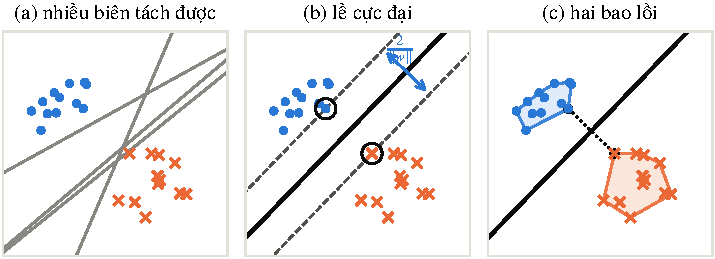
\includegraphics[width=\linewidth]{fig_hard_margin.pdf}
\caption[SVM lề cứng]{SVM lề cứng. (a) Dữ liệu tách được thường có nhiều siêu phẳng phân loại đúng. (b) Siêu phẳng lề cực đại (nét liền), hai siêu phẳng $w^\T x+w_0=\pm1$ (nét đứt) và các vectơ hỗ trợ (khoanh tròn); khoảng cách giữa hai nét đứt là $2/\|w\|$. (c) Cách nhìn đối ngẫu: siêu phẳng tối ưu là trung trực của đoạn nối hai điểm gần nhau nhất của hai bao lồi.}
\label{fig:hardmargin}
\end{figure}

% ----------------------------------------------------------------------------
\section{SVM lề mềm và hàm mất mát bản lề}\label{sec:softmargin}

Khi hai bao lồi giao nhau, bài toán~\eqref{eq:hard-primal} vô nghiệm (\cref{prop:hard-exist}). Dữ liệu thực tế hầu như luôn ở trong trường hợp này, do nhiễu hoặc do bản chất chồng lấn của hai lớp. Cortes và Vapnik~\cite{cortes1995} nới các ràng buộc bằng các \emph{biến bù} $e_k\ge0$ và phạt tổng các biến bù trong hàm mục tiêu:
\begin{equation}\label{eq:soft-primal}
\begin{aligned}
\min_{w,\,w_0,\,e}\quad & \frac12\|w\|^2+\gamma\sum_{k=1}^{N}e_k\\
\text{với điều kiện}\quad & y_k\bigl(w^\T x_k+w_0\bigr)\ge1-e_k,\ \ e_k\ge0,\qquad k=1,\dots,N,
\end{aligned}
\end{equation}
trong đó $\gamma>0$ là hằng số chính quy hóa, thường được gọi là $C$ trong các thư viện phần mềm; mô hình này được gọi là \emph{C-SVM}. Điểm $x_k$ với $e_k=0$ thỏa mãn ràng buộc lề như trước; điểm với $0<e_k<1$ nằm trong dải lề nhưng vẫn được phân loại đúng; điểm với $e_k>1$ bị phân loại sai (\cref{fig:softmargin}a).

\begin{proposition}\label{prop:hinge-form}
Bài toán~\eqref{eq:soft-primal} tương đương với bài toán không ràng buộc
\begin{equation}\label{eq:hinge-risk}
\min_{w,\,w_0}\ \frac12\|w\|^2+\gamma\sum_{k=1}^{N}\max\bigl\{0,\ 1-y_k(w^\T x_k+w_0)\bigr\}.
\end{equation}
\end{proposition}

\begin{proof}
Với $(w,w_0)$ cố định, giá trị nhỏ nhất của $e_k$ thỏa hai ràng buộc $e_k\ge1-y_k(w^\T x_k+w_0)$ và $e_k\ge0$ là $\max\{0,\,1-y_k(w^\T x_k+w_0)\}$; vì hàm mục tiêu tăng theo $e_k$, tại nghiệm $e_k$ nhận đúng giá trị đó.
\end{proof}

Hàm $\ell(t)=\max\{0,1-t\}=(1-t)_+$ được gọi là \emph{hàm mất mát bản lề}; nó chính là hàm bản lề của Mục~\ref{sec:pwl-functions}, dịch và lật. Dạng~\eqref{eq:hinge-risk} cho thấy C-SVM là một bài toán \emph{cực tiểu hóa rủi ro thực nghiệm có chính quy hóa}: số hạng thứ hai đo sai số trên dữ liệu, số hạng thứ nhất khống chế độ phức tạp của mô hình qua độ rộng của lề. Vì $(1-t)_+\ge\mathbf 1\{t\le0\}$, tổng các mất mát bản lề là một cận trên của số điểm huấn luyện bị phân loại sai; khác với mất mát $0$--$1$, nó là hàm lồi, nên bài toán~\eqref{eq:hinge-risk} là bài toán lồi (\cref{prop:convex-fn-ops}). \Cref{fig:softmargin}b so sánh ba hàm mất mát thường gặp.

\paragraph{Bài toán đối ngẫu.} Với các nhân tử $\alpha_k\ge0$ và $\mu_k\ge0$ cho hai nhóm ràng buộc, hàm Lagrange của~\eqref{eq:soft-primal} là
\[
L=\frac12\|w\|^2+\gamma\sum_ke_k-\sum_k\alpha_k\bigl[y_k(w^\T x_k+w_0)-1+e_k\bigr]-\sum_k\mu_ke_k .
\]
Điều kiện dừng theo $w$ và $w_0$ vẫn là~\eqref{eq:hard-stationarity}; điều kiện dừng theo $e_k$ cho $\gamma-\alpha_k-\mu_k=0$. Vì $\mu_k\ge0$, ta có $\alpha_k\le\gamma$, và các số hạng chứa $e_k$ triệt tiêu. Bài toán đối ngẫu của C-SVM vì vậy có cùng hàm mục tiêu với~\eqref{eq:hard-dual}, chỉ khác ở ràng buộc hộp:
\begin{equation}\label{eq:soft-dual}
\begin{aligned}
\max_{\alpha}\quad & \sum_{k=1}^{N}\alpha_k-\frac12\sum_{k=1}^{N}\sum_{l=1}^{N}\alpha_k\alpha_ly_ky_l\,x_k^\T x_l\\
\text{với điều kiện}\quad & 0\le\alpha_k\le\gamma,\ \ k=1,\dots,N;\qquad \sum_{k=1}^{N}\alpha_ky_k=0 .
\end{aligned}
\end{equation}
Bài toán gốc~\eqref{eq:soft-primal} luôn chấp nhận được (chọn $w=0$, $w_0=0$, $e_k=1$) và có ràng buộc affine, nên có đối ngẫu mạnh.

\paragraph{Ba loại điểm dữ liệu.} Hai điều kiện bù $\alpha_k\bigl[y_kf(x_k)-1+e_k\bigr]=0$ và $(\gamma-\alpha_k)e_k=0$, với $f(x)=w^{\ast\T}x+w_0^\ast$, chia dữ liệu thành ba loại:
\begin{enumerate}[label=(\roman*),leftmargin=2em]
\item $\alpha_k=0$: khi đó $\mu_k=\gamma>0$ nên $e_k=0$ và $y_kf(x_k)\ge1$. Điểm được phân loại đúng và nằm ngoài (hoặc trên) dải lề; nó không ảnh hưởng đến nghiệm.
\item $0<\alpha_k<\gamma$: khi đó $e_k=0$ và $y_kf(x_k)=1$. Điểm nằm đúng trên lề; các điểm loại này được dùng để tính $w_0^\ast=y_k-w^{\ast\T}x_k$.
\item $\alpha_k=\gamma$: khi đó $y_kf(x_k)=1-e_k\le1$. Điểm nằm trong dải lề hoặc bị phân loại sai.
\end{enumerate}
Các điểm loại (ii) và (iii) là các vectơ hỗ trợ. Hằng số $\gamma$ cân bằng giữa độ rộng của lề và số điểm vi phạm lề: $\gamma$ lớn phạt nặng các vi phạm và cho lề hẹp; khi dữ liệu tách được và $\gamma\to\infty$, ta trở lại SVM lề cứng. $\gamma$ nhỏ cho lề rộng và nhiều vectơ hỗ trợ hơn. Trong thực hành, $\gamma$ được chọn bằng kiểm định chéo (Chương~\ref{chap:3}).

\begin{figure}[t]
\centering
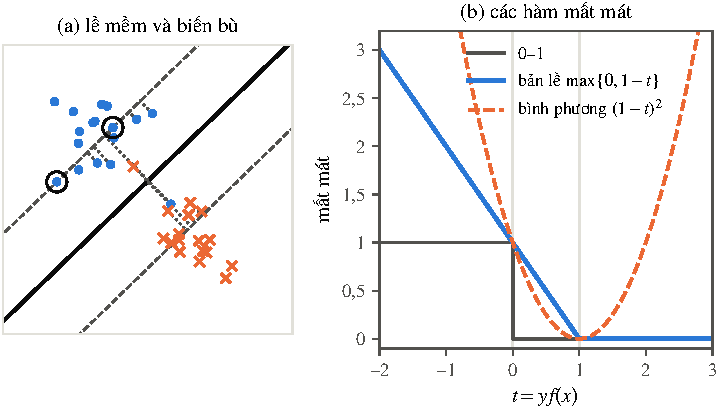
\includegraphics[width=\linewidth]{fig_soft_margin.pdf}
\caption[SVM lề mềm và các hàm mất mát]{(a) SVM lề mềm trên dữ liệu chồng lấn: các điểm vi phạm lề được nối bằng nét chấm tới siêu phẳng lề của lớp mình, độ dài nét chấm bằng $e_k/\|w\|$; khoanh tròn là các vectơ hỗ trợ nằm đúng trên lề. (b) Mất mát $0$--$1$, mất mát bản lề của C-SVM và mất mát bình phương của LS-SVM, theo $t=y\,f(x)$.}
\label{fig:softmargin}
\end{figure}

% ----------------------------------------------------------------------------
\section{Ánh xạ đặc trưng, hạt nhân và LS-SVM}\label{sec:kernel}

\subsection{Ánh xạ đặc trưng và thủ thuật hạt nhân}

Một bộ phân loại tuyến tính không thể tách hai vòng tròn đồng tâm (\cref{fig:lifting}a). Tuy nhiên, nếu thêm vào mỗi điểm tọa độ thứ ba $z=x(1)^2+x(2)^2$, tức là dùng ánh xạ $\varphi(x)=\bigl(x(1),x(2),x(1)^2+x(2)^2\bigr)$, thì trong $\R^3$ hai lớp được tách bởi một mặt phẳng $z=\text{hằng số}$ (\cref{fig:lifting}b). Tổng quát, cho một \emph{ánh xạ đặc trưng} $\varphi$ từ $\R^n$ vào một không gian đặc trưng $\mathcal F$ (hữu hạn hoặc vô hạn chiều, có tích vô hướng), ta áp dụng SVM tuyến tính cho dữ liệu $\{(\varphi(x_k),y_k)\}$. Bộ phân loại thu được, $\sgn\bigl(w^\T\varphi(x)+w_0\bigr)$, tuyến tính trong $\mathcal F$ nhưng phi tuyến trong $\R^n$.

\begin{figure}[t]
\centering
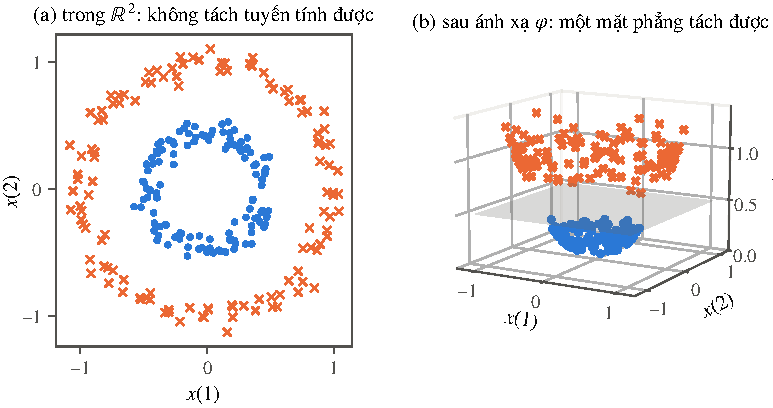
\includegraphics[width=\linewidth]{fig_lifting.pdf}
\caption[Ánh xạ đặc trưng biến dữ liệu không tách được thành tách được]{(a) Hai vòng tròn đồng tâm không tách tuyến tính được trong $\R^2$. (b) Sau ánh xạ $\varphi(x)=\bigl(x(1),x(2),z\bigr)$ với $z=x(1)^2+x(2)^2$, một mặt phẳng tách được hai lớp.}
\label{fig:lifting}
\end{figure}

Như đã nhận xét ở Mục~\ref{sec:hardmargin}, bài toán đối ngẫu~\eqref{eq:soft-dual} và bộ phân loại chỉ phụ thuộc vào dữ liệu qua các tích vô hướng. Vì vậy, sau khi thay $x_k$ bởi $\varphi(x_k)$, ta chỉ cần biết hàm
\begin{equation}\label{eq:kernel-def}
\kappa(x,z)=\varphi(x)^\T\varphi(z),
\end{equation}
gọi là \emph{hạt nhân}, mà không cần tính $\varphi$ một cách tường minh. Bài toán đối ngẫu có dạng~\eqref{eq:soft-dual} với $x_k^\T x_l$ thay bởi $\kappa(x_k,x_l)$, và bộ phân loại là
\begin{equation}\label{eq:kernel-classifier}
\hat y(x)=\sgn\Bigl(\sum_{k=1}^{N}\alpha_ky_k\,\kappa(x,x_k)+w_0\Bigr).
\end{equation}
Đây là \emph{thủ thuật hạt nhân}~\cite{boser1992,scholkopf2002}. Một hàm đối xứng $\kappa$ là hạt nhân, tức là viết được dưới dạng~\eqref{eq:kernel-def} với một ánh xạ $\varphi$ nào đó, khi và chỉ khi với mọi tập hữu hạn điểm $x_1,\dots,x_N$, ma trận $\bigl[\kappa(x_k,x_l)\bigr]_{k,l}$ là nửa xác định dương (điều kiện Mercer, xem~\cite[Chương~2]{scholkopf2002}). Ba hạt nhân thông dụng nhất là hạt nhân tuyến tính $\kappa(x,z)=x^\T z$, hạt nhân đa thức $\kappa(x,z)=(x^\T z+c)^d$ và hạt nhân Gauss (còn gọi là hạt nhân RBF)
\[
\kappa(x,z)=\exp\bigl(-\|x-z\|^2/\sigma^2\bigr),\qquad\sigma>0 .
\]

Với hạt nhân Gauss, không gian đặc trưng là vô hạn chiều, nên vectơ $w=\sum_k\alpha_ky_k\varphi(x_k)$ không thể được lưu một cách tường minh. Bộ phân loại~\eqref{eq:kernel-classifier} vì vậy phải lưu toàn bộ $N_s$ vectơ hỗ trợ, và mỗi lần dự đoán cần tính $N_s$ khoảng cách và $N_s$ hàm mũ. Với dữ liệu lớn, $N_s$ thường tỉ lệ với $N$, nên chi phí dự đoán và bộ nhớ tăng theo kích thước dữ liệu huấn luyện. Ngược lại, khi $\varphi$ tường minh và hữu hạn chiều, ta có thể tính $w$ một lần sau khi huấn luyện và dự đoán bằng một tích vô hướng trong $\R^M$. Nhận xét này là điểm xuất phát của PWL-SVM (Mục~\ref{sec:pwlsvm}).

\subsection{SVM bình phương tối thiểu}

Suykens và Vandewalle~\cite{suykens1999ls} đề xuất một biến thể của SVM trong đó ràng buộc bất đẳng thức được thay bằng đẳng thức và mất mát tuyến tính của biến bù được thay bằng mất mát bình phương:
\begin{equation}\label{eq:ls-primal}
\begin{aligned}
\min_{w,\,w_0,\,e}\quad & \frac12\|w\|^2+\frac{\gamma}{2}\sum_{k=1}^{N}e_k^2\\
\text{với điều kiện}\quad & y_k\bigl(w^\T\varphi(x_k)+w_0\bigr)=1-e_k,\qquad k=1,\dots,N .
\end{aligned}
\end{equation}
Mô hình này được gọi là \emph{LS-SVM}. Hàm Lagrange là
\[
L(w,w_0,e,\alpha)=\frac12\|w\|^2+\frac\gamma2\sum_ke_k^2-\sum_k\alpha_k\bigl[y_k\bigl(w^\T\varphi(x_k)+w_0\bigr)-1+e_k\bigr],
\]
với các nhân tử $\alpha_k\in\R$ không bị ràng buộc dấu (vì các ràng buộc là đẳng thức). Bài toán lồi với ràng buộc affine nên điều kiện KKT là cần và đủ (\cref{thm:kkt}):
\[
\begin{gathered}
w=\sum_k\alpha_ky_k\varphi(x_k),\qquad \sum_k\alpha_ky_k=0,\\
\alpha_k=\gamma e_k,\qquad y_k\bigl(w^\T\varphi(x_k)+w_0\bigr)=1-e_k,\qquad k=1,\dots,N.
\end{gathered}
\]
Thế đẳng thức thứ nhất và thứ ba vào đẳng thức cuối, ta được
\[
\sum_{l=1}^{N}y_ky_l\,\kappa(x_k,x_l)\,\alpha_l+y_kw_0+\frac{\alpha_k}{\gamma}=1,\qquad k=1,\dots,N;
\]
cùng với đẳng thức thứ hai, đó là hệ tuyến tính $(N+1)$ ẩn
\begin{equation}\label{eq:ls-dual}
\begin{bmatrix}0 & y^\T\\ y & \Theta+\gamma^{-1}I\end{bmatrix}
\begin{bmatrix}w_0\\ \alpha\end{bmatrix}
=\begin{bmatrix}0\\ \mathbf 1\end{bmatrix},\qquad \Theta_{kl}=y_ky_l\,\kappa(x_k,x_l),
\end{equation}
với $y=(y_1,\dots,y_N)^\T$ và $\mathbf 1\in\R^N$ là vectơ gồm toàn số $1$. Ma trận $\Theta$ nửa xác định dương, nên $H=\Theta+\gamma^{-1}I$ xác định dương; phần bù Schur $-y^\T H^{-1}y$ của khối $H$ âm, do đó ma trận của hệ~\eqref{eq:ls-dual} khả nghịch và hệ có nghiệm duy nhất. Bộ phân loại có dạng~\eqref{eq:kernel-classifier}.

So với C-SVM, LS-SVM đổi một bài toán quy hoạch toàn phương lấy một hệ phương trình tuyến tính, dễ giải và dễ cài đặt hơn. Đổi lại, vì $\alpha_k=\gamma e_k$ và $e_k$ nói chung khác $0$, gần như mọi điểm huấn luyện đều có nhân tử khác $0$: nghiệm không còn thưa, và với hạt nhân Gauss, bộ phân loại phải lưu toàn bộ $N$ điểm huấn luyện. \Cref{tab:csvm-lssvm} tóm tắt sự khác biệt giữa hai mô hình.

\begin{table}[t]
\centering
\caption[So sánh C-SVM và LS-SVM]{So sánh C-SVM và LS-SVM với một hạt nhân tổng quát.}
\label{tab:csvm-lssvm}
\small
\renewcommand{\arraystretch}{1.25}
\begin{tabularx}{\linewidth}{@{}l X X@{}}
\toprule
& \textbf{C-SVM} & \textbf{LS-SVM}\\
\midrule
Ràng buộc & bất đẳng thức, $e_k\ge0$ & đẳng thức\\
Mất mát & bản lề $(1-t)_+$ & bình phương $(1-t)^2$\\
Bài toán đối ngẫu & quy hoạch toàn phương với ràng buộc hộp & hệ tuyến tính $(N+1)$ ẩn\\
Tính thưa của nghiệm & chỉ các vectơ hỗ trợ có $\alpha_k\neq0$ & nói chung mọi $\alpha_k\neq0$\\
Công cụ giải điển hình & SMO~\cite{platt1999}, LIBSVM~\cite{chang2011} & phân tích Cholesky, gradient liên hợp\\
\bottomrule
\end{tabularx}
\end{table}

% ----------------------------------------------------------------------------
\section{Tập tuyến tính từng phần và phương trình tuyến tính từng phần}\label{sec:pwlset}

Trong bài toán phân loại hai lớp, miền dữ liệu được chia làm hai phần bởi một biên. Với bộ phân loại tuyến tính, biên là một siêu phẳng, tức là tập nghiệm của một phương trình tuyến tính $f(x)=0$, và điểm $x$ được xếp vào lớp $\sgn f(x)$. Theo Huang và cộng sự~\cite{huang2013}, ta gọi \emph{khả năng phân loại} của một họ bộ phân loại là mức độ phong phú về kiểu dáng của các biên mà họ đó tạo ra được. Theo nghĩa này, khả năng phân loại của bộ phân loại tuyến tính là rất hạn chế. Mở rộng đơn giản nhất của một siêu phẳng là một \emph{tập tuyến tính từng phần}: trên mỗi vùng của miền, tập đó trùng với một siêu phẳng.

Xét dữ liệu hai mặt trăng ở \cref{fig:moons}a. Hai lớp đan vào nhau nên không một đường thẳng nào tách được chúng, nhưng một đường gấp khúc gồm ba đoạn thẳng thì tách gần như hoàn hảo. Ta có thể mô tả đường gấp khúc này như sau. Chia hình vuông đơn vị thành ba dải ngang
\[
\Omega_k=\Bigl\{x\in[0,1]^2:\ \frac{k-1}{3}\le x(2)\le\frac{k}{3}\Bigr\},\qquad k=1,2,3;
\]
trên mỗi dải, biên là một đoạn của đường thẳng $c_k^\T x+d_k=0$ (\cref{fig:moons}b). Do đó
\[
\B=\bigcup_{k=1}^{3}\bigl\{x\in\Omega_k:\ c_k^\T x+d_k=0\bigr\}.
\]
Cách tìm các hệ số $c_k,d_k$ trong hình sẽ được trình bày ở Mục~\ref{sec:maps}; ở đây ta chỉ quan tâm đến cấu trúc của biên.

\begin{figure}[t]
\centering
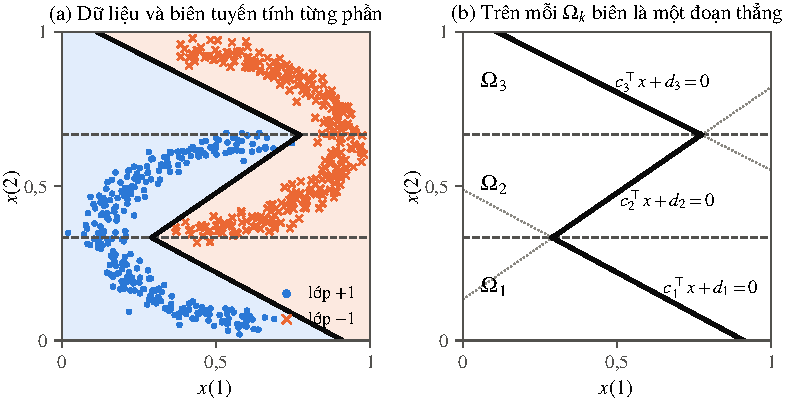
\includegraphics[width=\linewidth]{fig_moons_pwl.pdf}
\caption[Biên tuyến tính từng phần cho dữ liệu hai mặt trăng]{Một biên tuyến tính từng phần cho dữ liệu hai mặt trăng ($N=600$). (a) Biên gồm ba đoạn thẳng, tách đúng $599/600$ điểm. (b) Trên mỗi dải $\Omega_k$, biên trùng với một đoạn của đường thẳng $c_k^\T x+d_k=0$ (các phần kéo dài được vẽ bằng nét chấm). Dữ liệu và biên được tính bằng mã của đề án; ý tưởng theo Hình~1 của~\cite{huang2013}.}
\label{fig:moons}
\end{figure}

\begin{definition}[Tập tuyến tính từng phần~\cite{huang2013}]\label{def:pwlset}
Cho $\Omega\subseteq\R^n$. Tập $\B\subseteq\Omega$ được gọi là một \emph{tập tuyến tính từng phần} (tập PWL) nếu
\begin{enumerate}[label=(\roman*)]
\item có một phân hoạch đa diện $\{\Omega_1,\dots,\Omega_K\}$ của $\Omega$ (\cref{def:partition}), và
\item với mỗi $k$, tồn tại $c_k\in\R^n$ và $d_k\in\R$, không đồng thời bằng $0$, sao cho
\[
\B\cap\Omega_k=\bigl\{x\in\Omega_k:\ c_k^\T x+d_k=0\bigr\}.
\]
\end{enumerate}
\end{definition}

\begin{remark}\label{rem:pwlset}
Điều kiện “$x\in\Omega_k$” trong (ii) là cần thiết: thiếu nó, vế phải là cả một siêu phẳng, thường không nằm trong $\Omega_k$. Nếu $c_k=0$ thì $d_k\neq0$ và $\B\cap\Omega_k=\emptyset$, tức là biên không đi qua vùng $\Omega_k$; điều này cho phép các vùng “trống”. Điều kiện $(c_k,d_k)\neq(0,0)$ loại trừ trường hợp $\B$ chứa trọn một vùng, vì khi đó $\B$ không còn là một biên theo nghĩa thông thường.
\end{remark}

Định lý sau cho thấy mọi tập PWL đều là tập nghiệm của một phương trình tuyến tính từng phần, tương tự như siêu phẳng là tập nghiệm của một phương trình tuyến tính.

\begin{theorem}[\cite{huang2013}, Định lý~1]\label{thm:pwl-set}
Mọi tập tuyến tính từng phần $\B$ đều là tập nghiệm của một phương trình tuyến tính từng phần: tồn tại hàm PWL $f:\R^n\to\R$ sao cho $\B=\{x\in\R^n:\ f(x)=0\}$.
\end{theorem}

\begin{proof}
Dùng các ký hiệu của \cref{def:pwlset} và viết mỗi đa diện dưới dạng
\[
\Omega_k=\bigl\{x:\ a_{ki}^\T x+b_{ki}\le 0,\ i=1,\dots,I_k\bigr\},\qquad k=1,\dots,K .
\]
Với mỗi $k$, đặt
\begin{equation}\label{eq:gk}
g_k(x)=\max\Bigl\{\,|c_k^\T x+d_k|,\ \max_{1\le i\le I_k}\bigl(a_{ki}^\T x+b_{ki}\bigr)\Bigr\},
\qquad
f(x)=\min_{1\le k\le K} g_k(x).
\end{equation}
Theo \cref{prop:closure}, các hàm $g_k$ và $f$ là hàm PWL trên $\R^n$. Ta chứng minh hai khẳng định.

\emph{(a) $g_k(x)\ge0$ với mọi $x$, và $g_k(x)=0$ khi và chỉ khi $x\in\B\cap\Omega_k$.} Thật vậy, $g_k(x)\ge|c_k^\T x+d_k|\ge0$. Hơn nữa, $g_k(x)=0$ khi và chỉ khi $|c_k^\T x+d_k|\le0$ và $a_{ki}^\T x+b_{ki}\le0$ với mọi $i$, tức là khi và chỉ khi $c_k^\T x+d_k=0$ và $x\in\Omega_k$. Theo \cref{def:pwlset}(ii), điều đó tương đương với $x\in\B\cap\Omega_k$.

\emph{(b) $\{f=0\}=\B$.} Vì mọi $g_k$ đều không âm nên $f(x)=0$ khi và chỉ khi $g_k(x)=0$ với ít nhất một $k$. Kết hợp với (a) và việc $\B\subseteq\Omega=\bigcup_k\Omega_k$, ta được
\[
\{x:\ f(x)=0\}=\bigcup_{k=1}^{K}\bigl(\B\cap\Omega_k\bigr)=\B\cap\Omega=\B. \qedhere
\]
\end{proof}

\begin{remark}\label{rem:proof}
Chứng minh trong~\cite{huang2013} xét riêng hai chiều bao hàm và dùng thêm lập luận về phần trong của các vùng $\Omega_k$ để chỉ ra $g_k(x_0)\ge0$ khi $k\neq k_0$. Nhận xét đơn giản $g_k\ge|c_k^\T x+d_k|\ge0$ làm lập luận đó trở nên không cần thiết. Cũng từ chứng minh trên ta thấy điều kiện phần trong rời nhau của phân hoạch không được dùng đến; chỉ cần các vùng phủ $\Omega$.
\end{remark}

\begin{remark}\label{rem:nonneg}
Hàm $f$ trong~\eqref{eq:gk} không âm trên toàn $\R^n$, nên nó \emph{mô tả} biên $\B$ nhưng không phân biệt được hai phía của biên: $\sgn f$ không phải là một bộ phân loại. Để phân loại, ta cần một hàm đổi dấu khi đi qua $\B$. Nếu $\Omega\setminus\B$ gồm hai phần ứng với hai lớp và mỗi điểm của $\B$ đều là điểm biên chung của hai phần đó, thì đổi dấu $f$ trên phần ứng với lớp $-1$ ta được một hàm PWL liên tục, dương ở lớp $+1$, âm ở lớp $-1$ và có cùng tập không điểm $\B$. Trong PWL-SVM, hàm đổi dấu này không được xây dựng tường minh mà được tìm trực tiếp bằng một bài toán tối ưu; các định lý biểu diễn chỉ bảo đảm rằng họ hàm được tìm kiếm là đủ giàu.
\end{remark}

Vì $|t|=\max\{t,-t\}$ và $\max\{t_1,\max\{t_2,t_3\}\}=\max\{t_1,t_2,t_3\}$, hàm $f$ trong~\eqref{eq:gk} viết được dưới dạng min--max
\begin{equation}\label{eq:minmax}
f(x)=\min_{1\le k\le K}\ \max\bigl\{c_k^\T x+d_k,\ -c_k^\T x-d_k,\ a_{k1}^\T x+b_{k1},\dots,a_{kI_k}^\T x+b_{kI_k}\bigr\}.
\end{equation}
Từ dạng min--max, người ta có thể xây dựng bộ phân loại PWL bằng cách coi các hệ số $c_k,d_k,a_{ki},b_{ki}$ là ẩn và cực tiểu hóa một hàm mất mát trên dữ liệu. Tuy nhiên, bài toán thu được là không lồi và không trơn; trong thực nghiệm của phương pháp tách max--min, số vùng chỉ được xét đến $K\le5$~\cite{bagirov2005}. Để xác định tham số một cách hiệu quả và có khả năng tổng quát hóa tốt, Huang và cộng sự chuyển sang một dạng biểu diễn khác, tuyến tính theo tham số, dựa trên \cref{thm:wangsun}.

\begin{theorem}[\cite{huang2013}, Định lý~2]\label{thm:ghh-set}
Với mọi tập tuyến tính từng phần $\B\subseteq\R^n$, tồn tại số nguyên dương $D$, các hệ số $w_1,\dots,w_D\in\R$ và các tham số $p_{mi}\in\R^n$, $q_{mi}\in\R$ ($m=1,\dots,D$; $i=0,\dots,n$) sao cho
\begin{equation}\label{eq:ghh-set}
\B=\Bigl\{x:\ \sum_{m=1}^{D}w_m\,g_m(x)=0\Bigr\},\qquad
g_m(x)=\max_{0\le i\le n}\bigl\{p_{mi}^\T x+q_{mi}\bigr\}.
\end{equation}
\end{theorem}

\begin{proof}
Theo \cref{thm:pwl-set}, $\B=\{f=0\}$ với một hàm PWL $f$. Theo \cref{thm:wangsun}, $f=\sum_{m=1}^{D}\sigma_m\max\{\ell_{m,0},\dots,\ell_{m,n}\}$ với $\sigma_m\in\{-1,1\}$. Đặt $w_m=\sigma_m$ và gọi $p_{mi},q_{mi}$ là các hệ số của $\ell_{m,i}$, ta được~\eqref{eq:ghh-set}.
\end{proof}

Trong~\cite{huang2013}, định lý được suy ra qua một bước trung gian: biến dạng min--max~\eqref{eq:minmax} thành dạng max--min nhờ đẳng thức
$\min_k\max_i t_{ik}=-\max_k\min_i\,(-t_{ik})$,
rồi áp dụng kết quả của Wang và Sun cho dạng max--min. Hai cách lập luận là tương đương, vì theo \cref{thm:lattice}, mọi hàm PWL đều có dạng max--min.

% ----------------------------------------------------------------------------
\section{Ánh xạ đặc trưng tuyến tính từng phần và PWL-SVM}\label{sec:pwlsvm}

\subsection{Từ định lý biểu diễn đến ánh xạ đặc trưng}

\Cref{thm:ghh-set} biểu diễn biên PWL như tập không điểm của một \emph{tổ hợp tuyến tính} các hàm cơ sở $g_m$. Đó chính là dạng mà SVM có thể xử lý: nếu coi các $g_m$ là đặc trưng, thì việc tìm các hệ số $w_m$ là một bài toán phân loại tuyến tính. Trước khi làm điều đó, ta tách phần affine ra khỏi mỗi hàm cơ sở. Với mọi số thực $a_0,\dots,a_n$ ta có $\max_i a_i=a_0+\max\{0,\,a_1-a_0,\dots,a_n-a_0\}$. Áp dụng cho $g_m$, với $\tilde p_{mi}=p_{mi}-p_{m0}$ và $\tilde q_{mi}=q_{mi}-q_{m0}$:
\[
g_m(x)=\bigl(p_{m0}^\T x+q_{m0}\bigr)+\max\bigl\{0,\ \tilde p_{m1}^\T x+\tilde q_{m1},\ \dots,\ \tilde p_{mn}^\T x+\tilde q_{mn}\bigr\}.
\]
Lấy tổng theo $m$, phần affine gộp lại thành $\bigl(\sum_m w_m p_{m0}\bigr)^\T x+\sum_m w_m q_{m0}$, tức là một tổ hợp tuyến tính của các tọa độ $x(1),\dots,x(n)$ cộng với một hằng số. Hằng số này sẽ được hấp thụ vào hệ số chặn của SVM. Vì vậy, thay vì giữ nguyên các $g_m$, ta dùng ánh xạ đặc trưng $\varphi:\R^n\to\R^M$ với $M=n+D$ thành phần
\begin{equation}\label{eq:feature-map}
\varphi_m(x)=
\begin{cases}
x(m), & m=1,\dots,n,\\[2pt]
\max\bigl\{0,\,p_{m1}^\T x+q_{m1},\dots,p_{mn}^\T x+q_{mn}\bigr\}, & m=n+1,\dots,M,
\end{cases}
\end{equation}
trong đó, để đơn giản ký hiệu, ta viết lại $\tilde p,\tilde q$ thành $p,q$. Đây là ánh xạ (4) của bài báo gốc. Từ \cref{thm:ghh-set} ta suy ra ngay:

\begin{corollary}\label{cor:boundary}
Với mọi tập tuyến tính từng phần $\B\subseteq\R^n$, tồn tại số đặc trưng $M$, các tham số $p_{mi},q_{mi}$ của ánh xạ~\eqref{eq:feature-map} và các hệ số $w\in\R^M$, $w_0\in\R$ sao cho $\B=\{x:\ w^\T\varphi(x)+w_0=0\}$.
\end{corollary}

Ý nghĩa của hệ quả nằm ở chỗ: \emph{khi các tham số phi tuyến $p_{mi},q_{mi}$ đã được cố định, hàm quyết định $w^\T\varphi(x)+w_0$ là tuyến tính theo các ẩn $(w,w_0)$}. Toàn bộ tính phi tuyến nằm trong $\varphi$, còn việc học là tuyến tính. Vì vậy ta có thể dùng nguyên vẹn SVM tuyến tính trong không gian đặc trưng $\R^M$, với mọi ưu điểm của nó: bài toán lồi, nghiệm toàn cục, lý thuyết lề và các bộ giải hiệu quả.

\subsection{PWL-C-SVM}

Thay $x_k$ bởi $\varphi(x_k)$ trong bài toán SVM lề mềm (Mục~\ref{sec:softmargin}), ta được bài toán gốc của PWL-C-SVM:
\begin{equation}\label{eq:pwl-c-svm}
\begin{aligned}
\min_{w,\,w_0,\,e}\quad & \frac12\sum_{m=1}^{M}w_m^2+\gamma\sum_{k=1}^{N}e_k\\
\text{với điều kiện}\quad & y_k\Bigl(w_0+\sum_{m=1}^{M}w_m\varphi_m(x_k)\Bigr)\ge 1-e_k,\ \ e_k\ge0,\ \ k=1,\dots,N.
\end{aligned}
\end{equation}
Để tránh nhầm với các tham số của ánh xạ, hệ số chặn được ký hiệu là $w_0$. Lặp lại đúng các bước dẫn bài toán đối ngẫu ở Mục~\ref{sec:softmargin}, ta được
\begin{equation}\label{eq:pwl-c-dual}
\begin{aligned}
\max_{\alpha}\quad & \sum_{k=1}^{N}\alpha_k-\frac12\sum_{k=1}^{N}\sum_{l=1}^{N}y_ky_l\,\kappa(x_k,x_l)\,\alpha_k\alpha_l\\
\text{với điều kiện}\quad & \sum_{k=1}^{N}\alpha_ky_k=0,\qquad 0\le\alpha_k\le\gamma,\quad k=1,\dots,N,
\end{aligned}
\end{equation}
với hạt nhân hữu hạn hạng
\begin{equation}\label{eq:kernel}
\kappa(x,z)=\varphi(x)^\T\varphi(z)=\sum_{m=1}^{M}\varphi_m(x)\varphi_m(z).
\end{equation}
Từ nghiệm đối ngẫu, ta khôi phục $w=\sum_{k}\alpha_ky_k\varphi(x_k)$ và dùng bộ phân loại dạng gốc
\begin{equation}\label{eq:classifier}
\hat y(x)=\sgn\bigl(w^\T\varphi(x)+w_0\bigr).
\end{equation}

Bài toán gốc~\eqref{eq:pwl-c-svm} có $M+N+1$ biến, bài toán đối ngẫu~\eqref{eq:pwl-c-dual} có $N$ biến; vì vậy Huang và cộng sự đề nghị giải bài toán đối ngẫu rồi khôi phục $w$. Điểm khác biệt căn bản so với SVM hạt nhân Gauss nằm ở khâu \emph{dự đoán}: vì $\varphi$ là tường minh và hữu hạn chiều, bộ phân loại~\eqref{eq:classifier} chỉ cần lưu $w$, $w_0$ và các tham số của ánh xạ, không cần lưu các vectơ hỗ trợ. \Cref{tab:cost} so sánh chi phí lưu trữ và chi phí tính toán khi dự đoán một điểm mới.

\begin{table}[t]
\centering
\caption[Chi phí lưu trữ và chi phí dự đoán của các mô hình]{Số thực cần lưu và số phép tính khi dự đoán một điểm, không kể $2n$ số của phép chuẩn hóa dữ liệu mà mọi mô hình đều cần; $D=M-n$ là số đặc trưng bản lề (với dạng cộng tính, $D$ cũng là số nút), $N_s$ là số vectơ hỗ trợ.}
\label{tab:cost}
\small
\renewcommand{\arraystretch}{1.25}
\begin{tabularx}{\linewidth}{@{}l c X@{}}
\toprule
\textbf{Mô hình} & \textbf{Số thực cần lưu} & \textbf{Phép tính khi dự đoán}\\
\midrule
SVM tuyến tính & $n+1$ & $n$ phép nhân--cộng\\
PWL-SVM cộng tính & $M+D+1$ & $D$ phép trừ và $D$ phép $\max$; $M$ phép nhân--cộng\\
PWL-SVM HH & $D(n+1)+M+1$ & $Dn$ phép nhân--cộng và $D$ phép $\max$; $M$ phép nhân--cộng\\
PWL-SVM GHH & $Dn(n+1)+M+1$ & $Dn^2$ phép nhân--cộng và $Dn$ phép $\max$; $M$ phép nhân--cộng\\
SVM hạt nhân Gauss & $N_s(n+1)+1$ & $N_s$ khoảng cách ($\approx 2N_sn$ phép tính) và $N_s$ hàm mũ\\
\bottomrule
\end{tabularx}
\end{table}

Với dữ liệu Magic ($n=10$), bài báo gốc cho biết SVM hạt nhân Gauss cần $1013$ vectơ hỗ trợ, tức khoảng $1013\times11$ số thực, trong khi PWL-C-SVM với ánh xạ cộng tính chỉ cần khoảng $100$ số, với độ chính xác gần như nhau ($0{,}839$ so với $0{,}837$)~\cite{huang2013}. Chương~\ref{chap:3} sẽ đo lại các con số này bằng thực nghiệm của đề án.

\subsection{PWL-LS-SVM}

Áp dụng LS-SVM (Mục~\ref{sec:kernel}) cho ánh xạ~\eqref{eq:feature-map}, ta được PWL-LS-SVM:
\begin{equation}\label{eq:pwl-ls-svm}
\begin{aligned}
\min_{w,\,w_0,\,e}\quad & \frac12\sum_{m=1}^{M}w_m^2+\frac{\gamma}{2}\sum_{k=1}^{N}e_k^2\\
\text{với điều kiện}\quad & y_k\Bigl(w_0+\sum_{m=1}^{M}w_m\varphi_m(x_k)\Bigr)=1-e_k,\qquad k=1,\dots,N.
\end{aligned}
\end{equation}
Theo Mục~\ref{sec:kernel}, bài toán đối ngẫu của~\eqref{eq:pwl-ls-svm} là hệ tuyến tính $(N+1)$ ẩn
\begin{equation}\label{eq:pwl-ls-dual}
\begin{bmatrix}0 & y^\T\\ y & \Theta+\gamma^{-1}I\end{bmatrix}
\begin{bmatrix}w_0\\ \alpha\end{bmatrix}
=\begin{bmatrix}0\\ \mathbf 1\end{bmatrix},\qquad \Theta_{kl}=y_ky_l\,\kappa(x_k,x_l),
\end{equation}
với hạt nhân hữu hạn hạng~\eqref{eq:kernel}. Sau khi khử $e$, bài toán gốc có $M+1$ ẩn, còn bài toán đối ngẫu có $N+1$ ẩn; vì vậy dạng gốc có lợi hơn khi $M\le N$~\cite{huang2013}. Mệnh đề sau cho thấy dạng gốc thực chất là một bài toán quen thuộc.

\begin{proposition}\label{prop:ridge}
Với $y_k\in\{-1,1\}$, bài toán~\eqref{eq:pwl-ls-svm} tương đương với bài toán hồi quy ridge trên nhãn $\pm1$ với hệ số chặn không bị phạt:
\begin{equation}\label{eq:ridge}
\min_{w,\,w_0}\ \ \frac12\|w\|^2+\frac{\gamma}{2}\sum_{k=1}^{N}\bigl(y_k-w^\T\varphi(x_k)-w_0\bigr)^2 .
\end{equation}
Bài toán này có nghiệm duy nhất
\[
w=\bigl(\Phi_c^\T\Phi_c+\gamma^{-1}I\bigr)^{-1}\Phi_c^\T y_c,\qquad w_0=\bar y-\bar\varphi^\T w,
\]
trong đó $\bar\varphi=\frac1N\sum_k\varphi(x_k)$, $\bar y=\frac1N\sum_k y_k$, $\Phi_c$ là ma trận cỡ $N\times M$ có hàng thứ $k$ là $(\varphi(x_k)-\bar\varphi)^\T$ và $y_c$ là vectơ có thành phần thứ $k$ là $y_k-\bar y$.
\end{proposition}

\begin{proof}
Khử $e_k=1-y_k(w^\T\varphi(x_k)+w_0)$ từ ràng buộc. Vì $y_k^2=1$,
\[
e_k^2=y_k^2\,e_k^2=\bigl(y_k-y_k^2(w^\T\varphi(x_k)+w_0)\bigr)^2=\bigl(y_k-w^\T\varphi(x_k)-w_0\bigr)^2,
\]
nên~\eqref{eq:pwl-ls-svm} trở thành~\eqref{eq:ridge}. Gọi $J(w,w_0)$ là hàm mục tiêu của~\eqref{eq:ridge}. Với mọi $(u,v)\neq(0,0)$, dạng toàn phương của ma trận Hessian bằng $\|u\|^2+\gamma\sum_k(u^\T\varphi(x_k)+v)^2>0$, nên $J$ lồi chặt và có không quá một điểm cực tiểu. Cho đạo hàm theo $w_0$ bằng $0$ ta được $w_0=\bar y-\bar\varphi^\T w$; khi đó $y_k-w^\T\varphi(x_k)-w_0=(y_k-\bar y)-w^\T(\varphi(x_k)-\bar\varphi)$ và $J$ trở thành $\frac12\|w\|^2+\frac\gamma2\|y_c-\Phi_cw\|^2$. Cho gradient theo $w$ bằng $0$ ta được $(\Phi_c^\T\Phi_c+\gamma^{-1}I)w=\Phi_c^\T y_c$; ma trận vế trái xác định dương nên khả nghịch.
\end{proof}

Như vậy, khi $M\ll N$, PWL-LS-SVM chỉ cần lập ma trận $\Phi_c^\T\Phi_c$ cỡ $M\times M$ (chi phí $O(NM^2)$) và giải một hệ $M$ ẩn (chi phí $O(M^3)$), rẻ hơn nhiều so với hệ đối ngẫu cỡ $(N+1)\times(N+1)$. Mục~\ref{sec:impl} kiểm tra bằng số rằng hai cách giải cho cùng một nghiệm.

\subsection{Một cách nhìn khác: PWL-SVM như một mạng nơ-ron hai lớp}

Khi mỗi đặc trưng trong~\eqref{eq:feature-map} chỉ dùng một siêu phẳng, ta có $\varphi_m(x)=\max\{0,\,p_m^\T x+q_m\}$, tức là $\varphi_m(x)=\mathrm{ReLU}(p_m^\T x+q_m)$: đó chính là đầu ra của một nơ-ron ReLU; với dạng tổng quát, $\varphi_m$ là một nơ-ron maxout có một mảnh bằng $0$~\cite{goodfellow2013}. Do đó bộ phân loại~\eqref{eq:classifier} là một mạng nơ-ron hai lớp (\cref{fig:network}): lớp ẩn gồm $D$ nơ-ron với trọng số \emph{cố định}, cộng thêm các kết nối tắt từ đầu vào đến đầu ra; chỉ lớp ra được huấn luyện, và được huấn luyện bằng nguyên lý cực đại lề. Quan hệ giữa ánh xạ đặc trưng của SVM và lớp ẩn của mạng nơ-ron đã được Suykens và Vandewalle chỉ ra từ sớm~\cite{suykens1999mlp}. Cách nhìn này đặt PWL-SVM vào cùng họ với các mô hình có lớp ẩn ngẫu nhiên như máy học cực trị~\cite{huanggb2006} và đặc trưng ngẫu nhiên~\cite{rahimi2007}, và làm rõ sự đánh đổi so với mạng ReLU huấn luyện bằng lan truyền ngược: cố định lớp ẩn giúp bài toán trở nên lồi, nhưng mỗi nơ-ron đóng góp ít hơn vì không được điều chỉnh theo dữ liệu.

\begin{figure}[t]
\centering
\begin{tikzpicture}[x=1cm,y=1cm,>={Stealth[length=2.2mm]},
  inp/.style={circle,draw=inktwo,fill=white,minimum size=9.5mm,inner sep=0pt,font=\small},
  hid/.style={circle,draw=inktwo,fill=planback,minimum size=9.5mm,inner sep=0pt,font=\small},
  lab/.style={font=\footnotesize,align=center}]
  % inputs
  \node[inp] (x1) at (0,3.0) {$x(1)$};
  \node[inp] (x2) at (0,1.85) {$x(2)$};
  \node at (0,1.0) {$\vdots$};
  \node[inp] (xn) at (0,0) {$x(n)$};
  % hidden layer
  \node[hid] (h1) at (4,3.15) {$\varphi_{n+1}$};
  \node[hid] (h2) at (4,2.0) {$\varphi_{n+2}$};
  \node at (4,1.12) {$\vdots$};
  \node[hid] (hD) at (4,0.0) {$\varphi_{M}$};
  % output
  \node[circle,draw=inktwo,minimum size=11mm] (s) at (8.2,1.5) {$\Sigma$};
  \node[draw=inktwo,rounded corners=2pt,minimum height=8mm,font=\small] (sg) at (10.4,1.5) {$\sgn(\cdot)$};
  \node[font=\small] (y) at (12.2,1.5) {$\hat y(x)$};
  % input -> hidden (fixed weights)
  \foreach \a in {x1,x2,xn}{\foreach \b in {h1,h2,hD}{\draw[inktwo!45,line width=0.4pt] (\a) -- (\b);}}
  % hidden -> output (learned weights)
  \foreach \b in {h1,h2,hD}{\draw[->,line width=0.9pt] (\b) -- (s);}
  % skip connections routed around the hidden layer
  \draw[->,dashed,line width=0.8pt] (x1.north east) .. controls (1.6,4.55) and (6.4,4.55) .. (s.north west);
  \draw[->,dashed,line width=0.8pt] (xn.south east) .. controls (1.6,-1.45) and (6.4,-1.45) .. (s.south west);
  \draw[->] (s) -- (sg);
  \draw[->] (sg) -- (y);
  \node[font=\small] at (8.2,0.55) {$+\,w_0$};
  % hidden-layer frame and labels
  \begin{scope}[on background layer]
    \node[draw=planframe,dashed,rounded corners=3pt,fit=(h1)(hD),inner xsep=6pt,inner ysep=5pt] (box) {};
  \end{scope}
  \node[lab] at (4,4.72) {kết nối tắt: $x(1),\dots,x(n)$ đi thẳng tới đầu ra};
  \node[lab,text=planframe] at (4,-1.62) {lớp ẩn cố định: $p_m,q_m$ sinh ngẫu nhiên};
  \node[lab] at (6.15,-0.1) {trọng số $w$\\học bằng SVM};
\end{tikzpicture}
\caption[PWL-SVM nhìn như một mạng nơ-ron hai lớp]{PWL-SVM với ánh xạ siêu phẳng bản lề nhìn như một mạng nơ-ron hai lớp: lớp ẩn gồm các nơ-ron ReLU với tham số cố định; các tọa độ $x(1),\dots,x(n)$ đi thẳng đến đầu ra (nét đứt); chỉ các trọng số của lớp ra được học, bằng bài toán lồi~\eqref{eq:pwl-c-svm} hoặc~\eqref{eq:pwl-ls-svm}.}
\label{fig:network}
\end{figure}

% ----------------------------------------------------------------------------
\section{Các dạng ánh xạ đặc trưng và cách chọn tham số}\label{sec:maps}

Khả năng phân loại của PWL-SVM phụ thuộc vào dạng cụ thể của các đặc trưng $\varphi_m$ và vào cách chọn tham số của chúng. Mục này trình bày ba dạng ánh xạ được đề xuất trong~\cite{huang2013}, từ đơn giản đến tổng quát, và các quy tắc sinh tham số.

\subsection{Ba dạng ánh xạ}

\paragraph{Dạng cộng tính.} Đơn giản nhất là cho mỗi đặc trưng chỉ phụ thuộc vào một tọa độ:
\begin{equation}\label{eq:additive}
\varphi_m(x)=\max\{0,\ x(i_m)-q_m\},\qquad i_m\in\{1,\dots,n\},\ q_m\in\R .
\end{equation}
Gộp các số hạng theo từng tọa độ, hàm quyết định có dạng $w_0+\sum_{i=1}^{n}h_i\bigl(x(i)\bigr)$, trong đó theo \cref{prop:1d}, mỗi $h_i$ là một hàm PWL một biến với các điểm gãy là những $q_m$ ứng với $i_m=i$. Đây là một \emph{mô hình cộng tính} theo nghĩa của thống kê học~\cite{hastie1990}: ảnh hưởng của từng biến có thể vẽ ra và đọc được, một ưu điểm lớn về khả năng diễn giải. Đổi lại, biên các vùng tuyến tính là các siêu phẳng song song với trục tọa độ (\cref{fig:regions}a), và mô hình không biểu diễn được tương tác giữa các biến; Chương~\ref{chap:3} sẽ chỉ ra một hệ quả cụ thể của hạn chế này (\cref{prop:xor}).

\paragraph{Dạng siêu phẳng bản lề (HH).} Cho phép hướng tùy ý:
\begin{equation}\label{eq:hh}
\varphi_m(x)=\max\{0,\ p_m^\T x+q_m\},\qquad p_m\in\R^n,\ q_m\in\R .
\end{equation}
Mỗi đặc trưng đổi trạng thái trên cả một siêu phẳng $p_m^\T x+q_m=0$ cắt ngang miền, nên $D$ đặc trưng chia miền thành các ô của một \emph{sắp xếp siêu phẳng} (\cref{fig:regions}b). Trên mỗi ô, mọi hàm $w^\T\varphi(x)+w_0$ đều affine, nên số ô là một thước đo độ linh hoạt của biên. Trong mặt phẳng, $D$ đường thẳng ở vị trí tổng quát tạo ra đúng $1+D+\binom{D}{2}$ ô: đường thẳng thứ $j$ cắt $j-1$ đường trước tại $j-1$ điểm phân biệt nên bị chia thành $j$ đoạn, mỗi đoạn tách một ô cũ làm hai. Với $D=6$ như trong hình, ta được $22$ ô, nhiều hơn hẳn $16$ ô của dạng cộng tính với cùng số đặc trưng.

\paragraph{Dạng siêu phẳng bản lề tổng quát (GHH).} Dùng đúng dạng của~\eqref{eq:feature-map}:
\begin{equation}\label{eq:ghh-map}
\varphi_m(x)=\max\bigl\{0,\ p_{m1}^\T x+q_{m1},\ \dots,\ p_{mn}^\T x+q_{mn}\bigr\}.
\end{equation}
Mỗi đặc trưng có $n+1$ mảnh, và vùng tuyến tính của nó là các tập mà trên đó một mảnh xác định đạt cực đại (\cref{fig:regions}c). Theo \cref{cor:boundary}, đây là dạng đủ để biểu diễn mọi biên PWL; cái giá là số tham số của mỗi đặc trưng tăng gấp $n$ lần so với dạng HH (\cref{tab:cost}).

\begin{figure}[t]
\centering
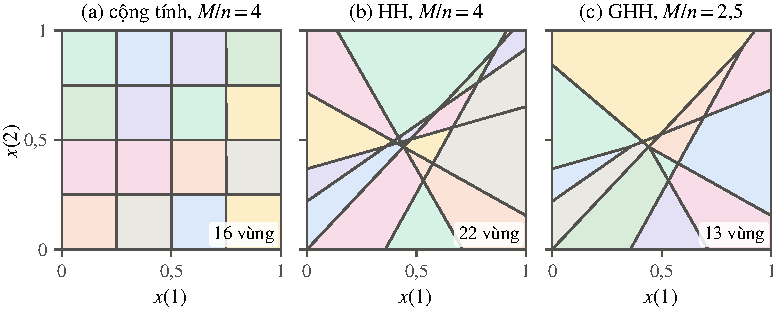
\includegraphics[width=\linewidth]{fig_regions_maps.pdf}
\caption[Phân vùng tuyến tính do ba dạng ánh xạ đặc trưng sinh ra]{Phân vùng tuyến tính của hình vuông đơn vị do ba dạng ánh xạ sinh ra: (a) cộng tính với lưới $4\times4$ (6 đặc trưng bản lề); (b) HH với 6 siêu phẳng ngẫu nhiên; (c) GHH với 3 đặc trưng, mỗi đặc trưng có 2 siêu phẳng. Trên mỗi vùng, mọi hàm quyết định $w^\T\varphi(x)+w_0$ đều là hàm affine.}
\label{fig:regions}
\end{figure}

\subsection{Chọn tham số}

Giống như tham số độ rộng của hạt nhân Gauss, các tham số phi tuyến của ánh xạ ảnh hưởng lớn đến kết quả nhưng khó tối ưu trực tiếp. Theo~\cite{huang2013}, ta chọn chúng dựa trên ý nghĩa hình học: các tham số của ánh xạ quyết định cấu trúc của các vùng, còn siêu phẳng trong từng vùng do SVM xác định. Trước hết, mỗi thành phần của dữ liệu được chuẩn hóa về đoạn $[0,1]$.

\emph{Với dạng cộng tính}, các nút $q_m$ được đặt đều trên mỗi trục: chia $[0,1]$ thành $S$ đoạn bằng nhau, ta được $S-1$ nút trên mỗi trục và $M=Sn$ đặc trưng (kể cả $n$ tọa độ). Bài báo gốc đề nghị $S=10$, tức $M=10n$~\cite{huang2013}.

\begin{remark}\label{rem:quantile}
Lưới đều ngầm giả định rằng dữ liệu trải tương đối đều trên mỗi trục. Với những biến lệch mạnh, chẳng hạn các số tiền trong dữ liệu tín dụng ở Mục~\ref{sec:application}, phần lớn dữ liệu dồn vào một hai đoạn đầu và các nút còn lại gần như vô dụng. Một lựa chọn tự nhiên là đặt nút tại các phân vị mẫu mức $s/S$, $s=1,\dots,S-1$, của từng biến, bỏ đi các nút trùng nhau ở những biến chỉ nhận ít giá trị. Mọi kết quả ở các mục trước vẫn giữ nguyên, vì các nút vẫn được cố định trước khi giải SVM.
\end{remark}

\emph{Với dạng HH và GHH}, các siêu phẳng được sinh ngẫu nhiên sao cho chắc chắn cắt qua miền dữ liệu. Để sinh một siêu phẳng $p^\T x+q=0$, ta lấy $n$ điểm $u_1,\dots,u_n$ theo phân phối đều trên $[0,1]^n$, chọn $p(1)\in\{-1,1\}$ với xác suất bằng nhau, rồi giải hệ $n$ phương trình
\begin{equation}\label{eq:random-plane}
\sum_{i=2}^{n}p(i)\,u_j(i)+q=-p(1)\,u_j(1),\qquad j=1,\dots,n,
\end{equation}
với $n$ ẩn $p(2),\dots,p(n),q$. Hàng thứ $j$ của ma trận hệ số trong~\eqref{eq:random-plane} là $\bigl(u_j(2),\dots,u_j(n),1\bigr)$. Ma trận này khả nghịch khi và chỉ khi các điểm $\tilde u_j=\bigl(u_j(2),\dots,u_j(n)\bigr)$, $j=1,\dots,n$, độc lập affine trong $\R^{n-1}$, điều xảy ra với xác suất $1$ vì các điểm được lấy theo một phân phối liên tục. Siêu phẳng thu được đi qua $n$ điểm của miền nên luôn cắt miền --- điều mà các siêu phẳng có hệ số lấy ngẫu nhiên tùy ý không bảo đảm. Dấu của $p(1)$ quyết định nửa không gian nào là nơi bản lề hoạt động. Với GHH, mỗi đặc trưng dùng $n$ siêu phẳng sinh độc lập theo cách này.

\begin{remark}\label{rem:scale}
Việc cố định $|p(1)|=1$ làm cho độ lớn $\|p\|$ rất khác nhau giữa các đặc trưng: một siêu phẳng gần song song với trục $x(1)$ có $|p(2)|,\dots,|p(n)|$ lớn, nên đặc trưng tương ứng có biên độ lớn. Do số hạng chính quy $\frac12\|w\|^2$ phạt mọi trọng số như nhau, đặc trưng có biên độ lớn thực chất bị phạt nhẹ hơn. Một lựa chọn khác là chuẩn hóa $\|p\|_2=1$; ảnh hưởng của lựa chọn này sẽ được kiểm tra ở Chương~\ref{chap:3}.
\end{remark}

\subsection{Hai ví dụ}

\emph{Trở lại dữ liệu hai mặt trăng.} Biết trước rằng biên cần đổi hướng khi $x(2)$ đi qua $\tfrac13$ và $\tfrac23$, ta dùng ánh xạ cộng tính với các nút chỉ đặt trên trục thứ hai:
\[
\varphi_1(x)=x(1),\quad \varphi_2(x)=x(2),\quad \varphi_3(x)=\bigl(x(2)-\tfrac13\bigr)_+,\quad \varphi_4(x)=\bigl(x(2)-\tfrac23\bigr)_+ .
\]
Giải PWL-C-SVM~\eqref{eq:pwl-c-svm} với $\gamma=100$ trên dữ liệu của \cref{fig:moons}, ta được hàm quyết định
\[
f(x)=7{,}98-8{,}76\,x(1)-16{,}33\,x(2)+29{,}03\bigl(x(2)-\tfrac13\bigr)_+-30{,}06\bigl(x(2)-\tfrac23\bigr)_+ .
\]
Trên mỗi dải $\Omega_k$, các số hạng bản lề hoặc bằng $0$ hoặc là hàm affine, nên $f$ là affine và biên $\{f=0\}\cap\Omega_k$ là một đoạn thẳng. Chẳng hạn trên $\Omega_2$ chỉ $\varphi_3$ hoạt động và $f(x)=-1{,}69-8{,}76\,x(1)+12{,}70\,x(2)$; đó là đường thẳng $c_2^\T x+d_2=0$ ở \cref{fig:moons}b. Bộ phân loại dùng $32$ vectơ hỗ trợ và phân loại đúng $599/600$ điểm huấn luyện. Ở ví dụ này, vị trí các nút được chọn nhờ biết trước hình dạng của dữ liệu; với dữ liệu “hộp đen”, ta dùng lưới đều hoặc siêu phẳng ngẫu nhiên như trên.

\emph{Một ánh xạ ngẫu nhiên, nhiều biên khác nhau.} Để thấy một ánh xạ cố định có thể sinh ra những biên đa dạng thế nào, xét ánh xạ HH trong $\R^2$ gồm $\varphi_1=x(1)$, $\varphi_2=x(2)$ và bốn đặc trưng bản lề được sinh theo quy trình~\eqref{eq:random-plane}:
\begin{equation}\label{eq:flex-map}
\begin{aligned}
\varphi_3(x)&=\bigl(x(1)+0{,}567\,x(2)-0{,}919\bigr)_+, \\
\varphi_4(x)&=\bigl(-x(1)-3{,}676\,x(2)+1{,}604\bigr)_+,\\
\varphi_5(x)&=\bigl(x(1)-3{,}171\,x(2)-0{,}089\bigr)_+, \\
\varphi_6(x)&=\bigl(-x(1)+0{,}654\,x(2)+0{,}074\bigr)_+.
\end{aligned}
\end{equation}
\Cref{fig:flex} vẽ biên $\{x:\ w_0+\sum_{m=1}^{6}w_m\varphi_m(x)=0\}$ với ba vectơ trọng số ở \cref{tab:flex}. Cùng một ánh xạ, chỉ thay đổi trọng số, ta được một biên lồi, một biên không lồi và một biên không liên thông. Nhiệm vụ của SVM là chọn ra, trong họ các biên đó, biên có lề lớn nhất trên dữ liệu.

\begin{figure}[t]
\centering
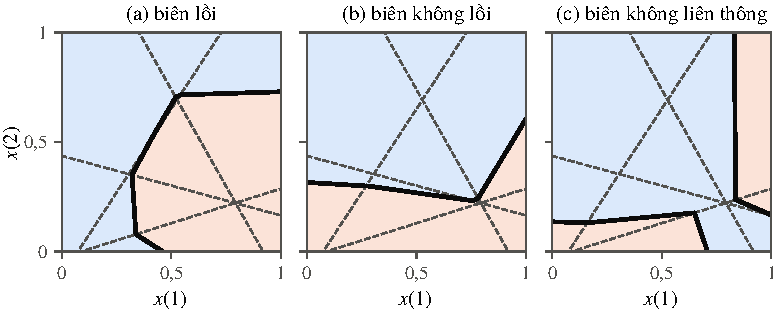
\includegraphics[width=\linewidth]{fig_flexibility.pdf}
\caption[Ba biên phân loại khác nhau sinh bởi cùng một ánh xạ HH]{Cùng ánh xạ~\eqref{eq:flex-map}, ba vectơ trọng số ở \cref{tab:flex} cho ba biên (nét liền) có hình dạng rất khác nhau. Nét đứt là bốn đường $\varphi_m(x)=0$, $m=3,\dots,6$; vùng tô cam là $\{f\le0\}$. Ví dụ được dựng lại theo ý tưởng của Hình~2 trong~\cite{huang2013}.}
\label{fig:flex}
\end{figure}

\begin{table}[t]
\centering
\caption[Ba vectơ trọng số cho cùng một ánh xạ HH]{Ba vectơ trọng số dùng ở \cref{fig:flex}.}
\label{tab:flex}
\small
\begin{tabular}{@{}l *{7}{S[table-format=-1.1]}@{}}
\toprule
& {$w_0$} & {$w_1$} & {$w_2$} & {$w_3$} & {$w_4$} & {$w_5$} & {$w_6$}\\
\midrule
(a) biên lồi & 0.4 & -3.0 & 1.6 & 2.9 & 0.5 & 1.1 & 1.9\\
(b) biên không lồi & 0.3 & -1.1 & 2.3 & -1.4 & -3.0 & 1.3 & 1.1\\
(c) biên không liên thông & 1.7 & -2.3 & 1.6 & -2.9 & -1.6 & 2.2 & -0.9\\
\bottomrule
\end{tabular}
\end{table}

\begin{remark}\label{rem:convex}
Biên ở \cref{fig:flex}a lồi không phải do tình cờ. Khi mọi hệ số của các đặc trưng bản lề đều không âm, $f$ là tổng của một hàm affine và các hàm lồi, nên $f$ lồi và tập $\{x:\ f(x)\le0\}$ là tập lồi. Vì vậy, thêm ràng buộc $w_m\ge0$ với $m>n$ vào~\eqref{eq:pwl-c-svm} là một cách đưa tri thức tiên nghiệm “một lớp nằm trong một tập lồi” vào mô hình mà vẫn giữ bài toán lồi, như đã được gợi ý trong~\cite[Mục~5]{huang2013}. Cần lưu ý rằng với $f$ lồi, tập lồi là tập mức dưới $\{f\le0\}$ chứ không phải $\{f\ge0\}$ như được viết trong~\cite{huang2013}; vì vậy lớp được biết là nằm trong một tập lồi phải được gán nhãn $-1$.
\end{remark}

% ----------------------------------------------------------------------------
% ----------------------------------------------------------------------------
\section{Quan hệ với các bộ phân loại tuyến tính từng phần khác}\label{sec:relations}

Nhiều bộ phân loại quen thuộc cho biên tuyến tính từng phần. Theo Mục~3 của~\cite{huang2013}, mục này chỉ ra rằng biên của ba bộ phân loại như vậy là biên của một PWL-SVM với tham số thích hợp. Các kết quả khẳng định \emph{khả năng biểu diễn} của họ PWL-SVM; chúng không nói rằng PWL-SVM với tham số sinh theo Mục~\ref{sec:maps} sẽ tìm được đúng các biên đó.

\subsection{SVM hạt nhân giao}

Hạt nhân giao $\kappa_\cap(x,z)=\sum_{i=1}^{n}\min\{x(i),z(i)\}$, xác định cho các vectơ có thành phần không âm, được dùng rộng rãi trong phân loại ảnh dựa trên lược đồ tần suất~\cite{maji2008}. Theo~\eqref{eq:kernel-classifier}, hàm quyết định của SVM với hạt nhân này (Ik-SVM) là $f(x)=\sum_k\alpha_ky_k\,\kappa_\cap(x,x_k)+w_0$.

\begin{proposition}\label{prop:iksvm}
Hàm quyết định của Ik-SVM là một hàm cộng tính tuyến tính từng phần:
\begin{equation}\label{eq:iksvm}
f(x)=w_0-\sum_{i=1}^{n}\sum_{k=1}^{N}\alpha_ky_k\,\bigl(x(i)-x_k(i)\bigr)_+ .
\end{equation}
Do đó mọi Ik-SVM là một PWL-SVM với ánh xạ cộng tính~\eqref{eq:additive}, trong đó các nút trên trục thứ $i$ là các giá trị $x_k(i)$ của dữ liệu huấn luyện.
\end{proposition}

\begin{proof}
Với mọi $a,b\in\R$ ta có $\min\{a,b\}=a-(a-b)_+$. Do đó
\[
\sum_k\alpha_ky_k\,\kappa_\cap(x,x_k)=\sum_{i=1}^{n}x(i)\sum_{k=1}^{N}\alpha_ky_k-\sum_{i=1}^{n}\sum_{k=1}^{N}\alpha_ky_k\bigl(x(i)-x_k(i)\bigr)_+ ,
\]
và số hạng thứ nhất bằng $0$ vì $\sum_k\alpha_ky_k=0$ là một ràng buộc của bài toán đối ngẫu~\eqref{eq:soft-dual}.
\end{proof}

Như vậy Ik-SVM thừa hưởng cả ưu điểm lẫn hạn chế của mô hình cộng tính: dễ diễn giải, nhưng không biểu diễn được tương tác giữa các biến. Hệ quả của hạn chế này sẽ được quan sát ở Mục~\ref{sec:exp2d}.

\subsection{AdaBoost với bộ phân loại yếu tuyến tính}

AdaBoost~\cite{freund1995} kết hợp các bộ phân loại yếu thành
\[
F(x)=\sum_{m=1}^{D}\eta_m\sgn(a_m^\T x+b_m),\qquad \eta_m>0,
\]
và phân loại theo $\sgn F(x)$. Khi các bộ phân loại yếu là tuyến tính, biên của AdaBoost là tuyến tính từng phần, nhưng $F$ không liên tục, nên biên không phải là tập không điểm của một hàm PWL liên tục. Huang và cộng sự thay hàm dấu bằng hàm xấp xỉ
\[
s_\delta(t)=-1+\frac1\delta(t+\delta)_+-\frac1\delta(t-\delta)_+,\qquad\delta>0,
\]
trùng với $\sgn(t)$ khi $|t|\ge\delta$ và tuyến tính trên đoạn $[-\delta,\delta]$.

\begin{proposition}\label{prop:adaboost}
Hàm $F_\delta(x)=\sum_m\eta_m\,s_\delta(a_m^\T x+b_m)$ là tổ hợp tuyến tính của một hằng số và các đặc trưng dạng siêu phẳng bản lề $\bigl(a_m^\T x+b_m\pm\delta\bigr)_+$, và $F_\delta(x)=F(x)$ với mọi $x$ nằm ngoài hợp các dải $S_m(\delta)=\{x:\ |a_m^\T x+b_m|<\delta\}$. Do đó $\sgn F_\delta$ và $\sgn F$ chỉ có thể khác nhau trên $\bigcup_mS_m(\delta)$, tập mà bề rộng của mỗi dải, $2\delta/\|a_m\|$, dần tới $0$ khi $\delta\to0$.
\end{proposition}

\begin{proof}
Khẳng định thứ nhất suy từ định nghĩa của $s_\delta$. Nếu $x\notin\bigcup_mS_m(\delta)$ thì $|a_m^\T x+b_m|\ge\delta$ với mọi $m$, nên $s_\delta(a_m^\T x+b_m)=\sgn(a_m^\T x+b_m)$ và $F_\delta(x)=F(x)$.
\end{proof}

Vậy PWL-SVM với ánh xạ HH xấp xỉ được biên của AdaBoost tuyến tính với độ chính xác tùy ý, theo nghĩa của \cref{prop:adaboost}.

\subsection{Phương pháp láng giềng gần nhất}

Với $k=1$, phương pháp láng giềng gần nhất~\cite{cover1967} gán cho $x$ nhãn của điểm huấn luyện gần $x$ nhất. Đặt $d_\pm(x)=\min_{k:\,y_k=\pm1}\|x-x_k\|^2$; điểm $x$ được xếp vào lớp $+1$ nếu $d_+(x)<d_-(x)$, và biên là tập $\{x:\ d_+(x)=d_-(x)\}$ (\cref{fig:knn}a).

\begin{proposition}\label{prop:knn}
Giả sử các điểm huấn luyện đôi một khác nhau. Khi đó $g=d_+-d_-$ là hàm PWL liên tục trên $\R^n$. Do đó biên của phương pháp một láng giềng gần nhất là tập không điểm của một hàm PWL, và theo \cref{cor:boundary} nó biểu diễn được bởi một PWL-SVM với ánh xạ~\eqref{eq:feature-map}.
\end{proposition}

\begin{proof}
Với mỗi cặp $(k,l)$ gồm một điểm lớp $+1$ và một điểm lớp $-1$, gọi $R_{kl}$ là tập các $x$ mà $x_k$ là điểm gần nhất trong lớp $+1$ và $x_l$ là điểm gần nhất trong lớp $-1$. Bất đẳng thức $\|x-x_k\|^2\le\|x-x_{k'}\|^2$ tương đương với $2(x_{k'}-x_k)^\T x\le\|x_{k'}\|^2-\|x_k\|^2$, tuyến tính theo $x$; vì vậy $R_{kl}$ là một đa diện. Các tập $R_{kl}$ phủ $\R^n$, và phần trong của chúng rời nhau vì các điểm huấn luyện khác nhau. Trên $R_{kl}$,
\[
g(x)=\|x-x_k\|^2-\|x-x_l\|^2=2(x_l-x_k)^\T x+\|x_k\|^2-\|x_l\|^2
\]
là một hàm affine: các số hạng bậc hai triệt tiêu. Cuối cùng $g$ liên tục vì $d_+$ và $d_-$ liên tục.
\end{proof}

Điều thú vị là $d_+$ và $d_-$ là các hàm bậc hai từng phần, nhưng hiệu của chúng là tuyến tính từng phần. \Cref{fig:knn} so sánh biên của 1-NN và của Ik-SVM trên cùng một bộ dữ liệu nhỏ: cả hai đều là đường gấp khúc, nhưng biên của Ik-SVM chỉ đổi hướng tại các đường thẳng song song với trục tọa độ đi qua các điểm dữ liệu, đúng như \cref{prop:iksvm} dự báo.

\begin{figure}[t]
\centering
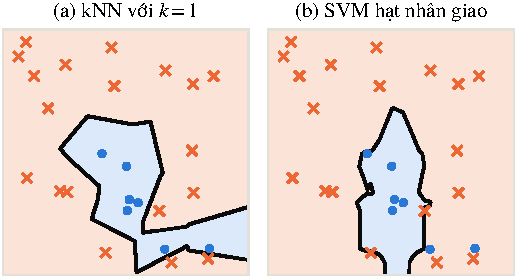
\includegraphics[width=0.72\linewidth]{fig_knn_iksvm.pdf}
\caption[Biên của 1-NN và của SVM hạt nhân giao]{Biên quyết định (nét liền) của (a) phương pháp một láng giềng gần nhất và (b) SVM hạt nhân giao trên cùng $26$ điểm dữ liệu. Cả hai biên đều tuyến tính từng phần.}
\label{fig:knn}
\end{figure}

\subsection{Ý nghĩa và giới hạn}

Ba kết quả trên cho thấy họ các biên mà PWL-SVM biểu diễn được chứa biên của Ik-SVM (với ánh xạ cộng tính), của AdaBoost tuyến tính (với ánh xạ HH, theo nghĩa xấp xỉ) và của 1-NN (với ánh xạ tổng quát). Huang và cộng sự rút ra rằng PWL-SVM “ít nhất có thể đạt được” hiệu năng của các bộ phân loại này~\cite{huang2013}. Nhận định đó cần được hiểu thận trọng. Các kết quả trên là về khả năng biểu diễn, với những tham số phi tuyến được chọn riêng cho từng trường hợp, chẳng hạn các nút tại mọi điểm dữ liệu; còn trong thực hành, PWL-SVM dùng tham số sinh theo quy tắc cố định ở Mục~\ref{sec:maps}. Khoảng cách giữa khả năng biểu diễn và độ chính xác thực tế sẽ được đo bằng thực nghiệm ở Chương~\ref{chap:3}.

% ----------------------------------------------------------------------------
\section*{Tiểu kết Chương 2}
\phantomsection\addcontentsline{toc}{section}{Tiểu kết Chương 2}

Chương 2 đã trình bày SVM từ lề cứng đến lề mềm, thủ thuật hạt nhân và LS-SVM, rồi xây dựng PWL-SVM theo một chuỗi lập luận chặt chẽ: mọi biên tuyến tính từng phần là tập không điểm của một hàm PWL liên tục (\cref{thm:pwl-set}); hàm đó là tổ hợp tuyến tính của các hàm bản lề tổng quát (\cref{thm:ghh-set}); tách phần affine ra, ta được ánh xạ đặc trưng~\eqref{eq:feature-map}, và việc học biên quy về một SVM tuyến tính trên $\varphi(x)$ (\cref{cor:boundary}). Mô hình thu được giữ tính lồi của SVM, có hai dạng PWL-C-SVM và PWL-LS-SVM, trong đó dạng gốc của PWL-LS-SVM chính là hồi quy ridge (\cref{prop:ridge}). Ưu điểm dự kiến nằm ở khâu dự đoán: mô hình chỉ cần lưu $w$ và tham số của ánh xạ (\cref{tab:cost}). Ba dạng ánh xạ cộng tính, HH và GHH đánh đổi giữa khả năng diễn giải, chi phí và độ linh hoạt; dạng cộng tính không biểu diễn được tương tác giữa các biến. Những câu hỏi còn để ngỏ --- chọn dạng ánh xạ nào, bao nhiêu đặc trưng, và độ chính xác, chi phí so với SVM hạt nhân Gauss ra sao --- được trả lời bằng thực nghiệm ở Chương~\ref{chap:3}.

% ============================================================================
%  CHƯƠNG 3. CÀI ĐẶT, THỰC NGHIỆM VÀ ỨNG DỤNG
% ============================================================================
\chapter{Cài đặt, thực nghiệm và ứng dụng}\label{chap:3}

Chương này kiểm nghiệm các kết quả lý thuyết của Chương~\ref{chap:2} bằng thực nghiệm và trả lời bốn câu hỏi nghiên cứu nêu ở Mở đầu. \Cref{sec:impl} mô tả phần cài đặt và các phép kiểm chứng số. \Cref{sec:exp2d} dùng dữ liệu hai chiều để quan sát trực tiếp biên quyết định. \Cref{sec:benchmark} tái hiện một thí nghiệm của bài báo gốc, so sánh ba biến thể PWL-SVM với sáu phương pháp khác trên mười bộ dữ liệu chuẩn và khảo sát ảnh hưởng của số đặc trưng cùng quy tắc chọn tham số. \Cref{sec:cost} đo chi phí huấn luyện, dự đoán và bộ nhớ. \Cref{sec:application} áp dụng PWL-SVM vào bài toán dự báo vỡ nợ thẻ tín dụng: so sánh với thẻ điểm truyền thống và các mô hình phi tuyến, phân tích khả năng diễn giải, và bổ sung ràng buộc đơn điệu. \Cref{sec:discussion} tổng hợp và thảo luận các kết quả.

% ----------------------------------------------------------------------------
\section{Cài đặt}\label{sec:impl}

Toàn bộ thực nghiệm được cài đặt bằng Python~3 với các thư viện NumPy~\cite{harris2020}, SciPy~\cite{virtanen2020} và scikit-learn~\cite{pedregosa2011}. Mã nguồn gồm một mô-đun chính, \texttt{pwlsvm.py}, với hai lớp tuân theo giao diện \texttt{fit}/\texttt{predict} của scikit-learn; nhờ vậy có thể dùng trực tiếp các công cụ kiểm định chéo và tìm kiếm tham số của thư viện này.
\begin{itemize}
\item Lớp \texttt{PWLFeatures} sinh tham số và tính ánh xạ đặc trưng~\eqref{eq:feature-map} cho ba dạng cộng tính, HH và GHH, theo đúng quy trình ở Mục~\ref{sec:maps}. Ngoài quy tắc của bài báo gốc, lớp này có hai tùy chọn: đặt nút của dạng cộng tính theo phân vị (\cref{rem:quantile}) và chuẩn hóa các siêu phẳng ngẫu nhiên về $\|p\|_2=1$ (\cref{rem:scale}).
\item Lớp \texttt{PWLSVM} ghép ba bước: chuẩn hóa từng thành phần về $[0,1]$ (giá trị nhỏ nhất, lớn nhất được học trên tập huấn luyện), tính $\varphi(x)$, và giải bài toán tuyến tính trên $\varphi(x)$. Với PWL-C-SVM có hai bộ giải. LIBSVM~\cite{chang2011} giải đúng bài toán đối ngẫu~\eqref{eq:pwl-c-dual} với hệ số chặn không bị phạt; nó được dùng cho các thí nghiệm nhỏ ở \cref{sec:exp2d} và \cref{sec:cosexp}. LIBLINEAR~\cite{fan2008} giải bài toán trên đặc trưng tường minh bằng phương pháp hạ theo tọa độ trên bài toán đối ngẫu, nhanh hơn nhiều khi $N$ hoặc $\gamma$ lớn; hệ số chặn được đưa vào như trọng số của một đặc trưng hằng bằng $10$ nên bị chính quy hóa nhẹ, với phạt tương đương $w_0^2/200$. LIBLINEAR được dùng cho mọi thí nghiệm còn lại. Với PWL-LS-SVM, dạng gốc được giải trực tiếp theo \cref{prop:ridge}.
\end{itemize}
Mô-đun thứ hai, \texttt{pwlsvm\_monotone.py}, bổ sung ràng buộc đơn điệu cho PWL-LS-SVM cộng tính (Mục~\ref{sec:monotone}). Các phương pháp đối chứng --- SVM tuyến tính, SVM và LS-SVM hạt nhân Gauss, SVM hạt nhân giao, kNN, mạng nơ-ron một lớp ẩn ReLU, và trong phần ứng dụng thêm hồi quy logistic, thẻ điểm logistic trên biến rời rạc hóa và tổ hợp cây tăng cường --- được đặt trong cùng một khung, để mọi phương pháp dùng chung cách chuẩn hóa, cách chia dữ liệu và cách chọn tham số. Quy trình huấn luyện và dự đoán của PWL-SVM được tóm tắt trong \cref{alg:pwlsvm}.

\begin{algorithm}[t]
\caption{Huấn luyện và dự đoán với PWL-SVM}\label{alg:pwlsvm}
\begin{algorithmic}[1]
\Require dữ liệu $\{(x_k,y_k)\}_{k=1}^{N}$; dạng ánh xạ (cộng tính, HH hoặc GHH); số đặc trưng trên mỗi chiều $M/n$; hằng số $\gamma$
\Ensure trọng số $w\in\R^M$, hệ số chặn $w_0$, tham số của ánh xạ và của phép chuẩn hóa
\State Chuẩn hóa từng thành phần của $x_k$ về $[0,1]$; lưu giá trị nhỏ nhất và lớn nhất
\If{dạng cộng tính}
  \State đặt $S=M/n$ và các nút $q=s/S$ ($s=1,\dots,S-1$), hoặc các phân vị mức $s/S$, trên mỗi trục
\Else
  \For{$m=n+1,\dots,M$}
    \State sinh $1$ siêu phẳng (HH) hoặc $n$ siêu phẳng (GHH) theo~\eqref{eq:random-plane}
  \EndFor
\EndIf
\State Lập ma trận $\Phi\in\R^{N\times M}$ có hàng thứ $k$ là $\varphi(x_k)^\T$, theo~\eqref{eq:feature-map}
\State Giải~\eqref{eq:pwl-c-dual} rồi tính $w=\sum_k\alpha_ky_k\varphi(x_k)$ (PWL-C-SVM), hoặc giải~\eqref{eq:ridge} (PWL-LS-SVM)
\State \textbf{Dự đoán} điểm mới $x$: chuẩn hóa $x$ bằng các giá trị đã lưu, trả về $\sgn\bigl(w^\T\varphi(x)+w_0\bigr)$
\end{algorithmic}
\end{algorithm}

\paragraph{Kiểm chứng tính đúng đắn.} Trước khi dùng mã cho thực nghiệm, đề án kiểm tra bằng số hai hệ thức của Chương~\ref{chap:2}, trên dữ liệu hai mặt trăng ($N=400$, $M=20$, $\gamma=10$) với cả ba dạng ánh xạ.
\begin{enumerate}[label=(\roman*)]
\item Với PWL-LS-SVM, nghiệm của dạng gốc (hồi quy ridge, \cref{prop:ridge}) và nghiệm của hệ đối ngẫu~\eqref{eq:pwl-ls-dual} phải trùng nhau. Sai khác lớn nhất giữa hai bộ tham số $(w,w_0)$ là $7\cdot10^{-12}$; trên $400$ điểm kiểm tra, giá trị hàm quyết định của hai lời giải sai khác không quá $2\cdot10^{-12}$. Hai cách giải cho cùng một nghiệm, chỉ khác nhau ở sai số làm tròn.
\item Với PWL-C-SVM, khôi phục $w=\sum_k\alpha_ky_k\varphi(x_k)$ từ nghiệm đối ngẫu với hạt nhân hữu hạn hạng~\eqref{eq:kernel} cho vectơ trọng số trùng với vectơ thu được khi giải trực tiếp trên $\varphi(x)$ (sai khác dưới $2\cdot10^{-12}$); hai bộ phân loại dự đoán giống hệt nhau trên toàn bộ tập kiểm tra.
\end{enumerate}
Ngoài ra, ví dụ hai mặt trăng ở Mục~\ref{sec:maps} tái hiện đúng hiện tượng mà bài báo gốc mô tả: bốn đặc trưng cộng tính cho một biên ba đoạn với các điểm gãy nằm trên hai đường $x(2)=\tfrac13$ và $x(2)=\tfrac23$.

% ----------------------------------------------------------------------------
\section{Thực nghiệm minh họa trên dữ liệu hai chiều}\label{sec:exp2d}

Với dữ liệu hai chiều, ta nhìn được trực tiếp biên quyết định, nên đây là nơi thích hợp để kiểm tra các nhận định định tính ở Chương~\ref{chap:2}. Đề án dùng bốn bộ dữ liệu tổng hợp có độ khó tăng dần (\cref{fig:demo2d}): hai mặt trăng (nhiễu Gauss với độ lệch chuẩn $0{,}15$), hai vòng tròn đồng tâm (tỉ số bán kính $0{,}5$, nhiễu $0{,}08$), bàn cờ $4\times4$ với các điểm phân bố đều, và hai xoắn ốc lồng nhau ($1{,}6$ vòng, nhiễu $0{,}06$). Mỗi bộ gồm $1000$ điểm, chia đôi thành $500$ điểm huấn luyện và $500$ điểm kiểm tra như trong bài báo gốc.

Năm phương pháp được so sánh: SVM tuyến tính; PWL-C-SVM với ánh xạ cộng tính ($M/n=10$), HH ($M/n=50$, tức $98$ siêu phẳng) và GHH ($M/n=25$, tức $48$ đặc trưng với tổng cộng $96$ siêu phẳng); và SVM hạt nhân Gauss. Hai cấu hình HH và GHH được chọn để có số siêu phẳng xấp xỉ nhau. Hằng số $\gamma$ được chọn trong tập $\{2^{-3},2^{-1},\dots,2^{11}\}$ bằng kiểm định chéo $5$ phần trên tập huấn luyện; với SVM hạt nhân Gauss, tham số $1/\sigma^2$ được chọn đồng thời trong $\{2^{-3},2^{-1},\dots,2^{9}\}$. Toàn bộ quy trình được lặp lại $10$ lần với dữ liệu và tham số ngẫu nhiên khác nhau; \cref{tab:exp2d} báo cáo trung bình và độ lệch chuẩn.

\begin{figure}[p]
\centering
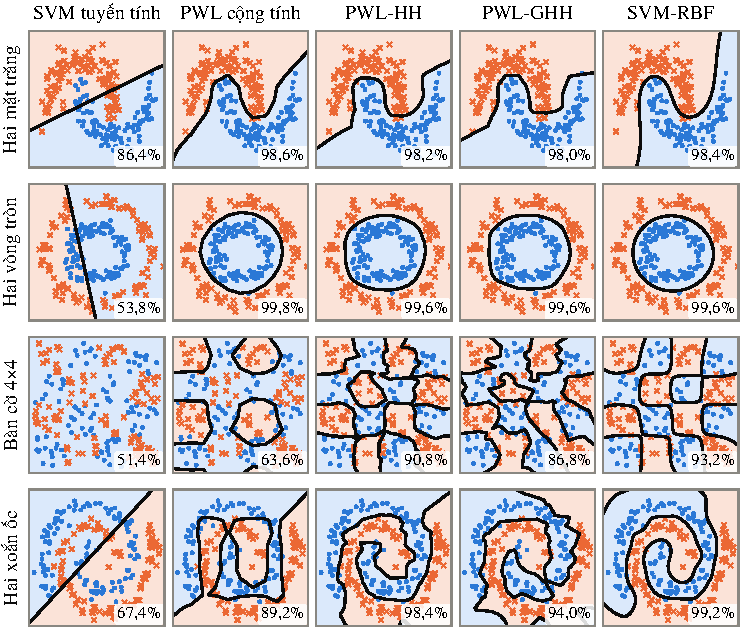
\includegraphics[width=\linewidth]{fig_demo_2d.pdf}
\caption[Biên quyết định của năm phương pháp trên dữ liệu hai chiều]{Biên quyết định của năm phương pháp trên bốn bộ dữ liệu hai chiều (lần lặp đầu tiên). Chấm xanh và dấu nhân cam là các điểm kiểm tra của hai lớp; con số ở góc là độ chính xác trên $500$ điểm kiểm tra. Biên của PWL-SVM là các đường gấp khúc, biên của SVM hạt nhân Gauss là đường trơn.}
\label{fig:demo2d}
\end{figure}

\begin{table}[t]
\centering
\caption[Độ chính xác trên dữ liệu hai chiều]{Độ chính xác trên tập kiểm tra (\%, trung bình $\pm$ độ lệch chuẩn qua $10$ lần lặp) trên dữ liệu hai chiều; in đậm là giá trị trung bình cao nhất mỗi hàng.}
\label{tab:exp2d}
\small
\renewcommand{\arraystretch}{1.2}
\setlength{\tabcolsep}{4pt}
\begin{tabular}{@{}l c c c c c@{}}
\toprule
\textbf{Dữ liệu} & \textbf{SVM tuyến tính} & \textbf{PWL cộng tính} & \textbf{PWL-HH} & \textbf{PWL-GHH} & \textbf{SVM-RBF}\\
\midrule
Hai mặt trăng & $87{,}3\pm2{,}0$ & $98{,}8\pm0{,}7$ & $98{,}7\pm0{,}7$ & $98{,}6\pm0{,}8$ & $\mathbf{98{,}9}\pm0{,}6$\\
Hai vòng tròn & $52{,}7\pm3{,}5$ & $\mathbf{99{,}9}\pm0{,}1$ & $99{,}8\pm0{,}2$ & $99{,}8\pm0{,}2$ & $99{,}8\pm0{,}2$\\
Bàn cờ $4\times4$ & $50{,}0\pm2{,}4$ & $55{,}5\pm3{,}4$ & $90{,}6\pm2{,}2$ & $85{,}7\pm2{,}5$ & $\mathbf{94{,}8}\pm1{,}2$\\
Hai xoắn ốc & $64{,}8\pm2{,}7$ & $89{,}2\pm1{,}5$ & $98{,}2\pm0{,}6$ & $96{,}7\pm1{,}4$ & $\mathbf{99{,}2}\pm0{,}4$\\
\bottomrule
\end{tabular}
\end{table}

Kết quả ở \cref{tab:exp2d} và \cref{fig:demo2d} phù hợp với phân tích ở Mục~\ref{sec:maps}. SVM tuyến tính thất bại trên cả bốn bộ; trên hai vòng tròn và bàn cờ, độ chính xác của nó xấp xỉ $50\%$, tức không hơn đoán ngẫu nhiên. Cả ba dạng PWL-SVM đều cải thiện rõ rệt, và trên hai mặt trăng, hai vòng tròn, chúng đạt độ chính xác ngang SVM hạt nhân Gauss, với sai khác nhỏ hơn độ lệch chuẩn.

Ánh xạ cộng tính cho kết quả gần như tuyệt đối trên hai vòng tròn ($99{,}9\%$) nhưng gần như thất bại trên bàn cờ ($55{,}5\%$). Nguyên nhân không nằm ở số đặc trưng mà ở cấu trúc của mô hình. Biên của hai vòng tròn là đường $x(1)^2+x(2)^2=r^2$, với vế trái là tổng của hai hàm một biến, nên một mô hình cộng tính xấp xỉ được dễ dàng. Ngược lại, mệnh đề sau cho thấy không mô hình cộng tính nào xử lý được cấu trúc kiểu bàn cờ.

\begin{proposition}\label{prop:xor}
Cho $a\neq b$ và $c\neq d$. Giả sử hai điểm $(a,c)$ và $(b,d)$ thuộc lớp $+1$, còn hai điểm $(a,d)$ và $(b,c)$ thuộc lớp $-1$. Khi đó không tồn tại hai hàm $g_1,g_2:\R\to\R$ nào sao cho hàm cộng tính $f(x)=g_1\bigl(x(1)\bigr)+g_2\bigl(x(2)\bigr)$ phân loại đúng cả bốn điểm.
\end{proposition}

\begin{proof}
Nếu có, thì $f(a,c)+f(b,d)>0$ và $f(a,d)+f(b,c)<0$. Nhưng cả hai tổng đều bằng $g_1(a)+g_1(b)+g_2(c)+g_2(d)$, mâu thuẫn.
\end{proof}

Bàn cờ $4\times4$ chứa rất nhiều bộ bốn điểm như vậy, nên mọi bộ phân loại cộng tính, dù dùng bao nhiêu đặc trưng, đều mắc nhiều lỗi. Kết luận này áp dụng cả cho SVM hạt nhân giao, vì theo Mục~\ref{sec:relations} nó cũng là một mô hình cộng tính; điều đó giải thích vì sao trong bài báo gốc, SVM hạt nhân giao chỉ đạt $48{,}8\%$ trên dữ liệu bàn cờ~\cite[Bảng~1]{huang2013}.

Hai dạng HH và GHH, vốn dùng các siêu phẳng có hướng tùy ý, xử lý được cả bàn cờ lẫn xoắn ốc. Trên hai bộ khó này, chúng vẫn kém SVM hạt nhân Gauss vài điểm phần trăm ($90{,}6\%$ và $85{,}7\%$ so với $94{,}8\%$ trên bàn cờ), và biên của chúng gấp khúc thay vì trơn. Với cùng số siêu phẳng, GHH kém HH một chút: mỗi đặc trưng GHH linh hoạt hơn, nhưng số trọng số được học chỉ bằng một nửa ($50$ so với $100$), trong khi các siêu phẳng ngẫu nhiên không được điều chỉnh theo dữ liệu. Nói cách khác, khả năng biểu diễn tổng quát của GHH (\cref{cor:boundary}) không tự động chuyển thành độ chính xác khi tham số được sinh ngẫu nhiên.

Một nhận xét về quy trình thực nghiệm: trên bàn cờ, hằng số $\gamma$ được chọn thường nằm ở đầu trên của lưới ($2^{9}$ hoặc $2^{11}$), và thời gian chọn tham số của PWL-HH và PWL-GHH (khoảng $9$ và $18$ giây mỗi lần lặp) lớn hơn nhiều so với SVM hạt nhân Gauss (dưới $0{,}4$ giây), vì LIBSVM hội tụ chậm khi $\gamma$ lớn. Đây là lý do các thí nghiệm trên dữ liệu chuẩn ở \cref{sec:benchmark} dùng bộ giải LIBLINEAR.

% ----------------------------------------------------------------------------

% ----------------------------------------------------------------------------
\section{Thực nghiệm trên dữ liệu chuẩn}\label{sec:benchmark}
% ----------------------------------------------------------------------------
%  3.3  Thực nghiệm trên dữ liệu chuẩn
% ----------------------------------------------------------------------------
\subsection{Tái hiện thí nghiệm trên dữ liệu Cosexp}\label{sec:cosexp}

Bộ dữ liệu Cosexp của hộp công cụ SVM-KM~\cite{canu2005} được bài báo gốc dùng để minh họa ảnh hưởng của số đặc trưng $M$. Các điểm được lấy đều trên miền $[0,5]\times[-1,1]$ và được gán nhãn theo dấu của $\cos\bigl(0{,}5\,e^{0{,}7x(1)}\bigr)-x(2)$; biên thật là đường cong $x(2)=\cos\bigl(0{,}5\,e^{0{,}7x(1)}\bigr)$, dao động ngày càng nhanh khi $x(1)$ tăng (nét đứt ở \cref{fig:cosexp}a,b). Theo đúng thiết lập của~\cite{huang2013}, ta dùng $500$ điểm huấn luyện, $500$ điểm kiểm tra và PWL-C-SVM với ánh xạ cộng tính, cho $M$ chạy từ $2$ đến $40$. Khác với bài báo, mỗi cấu hình được lặp lại trên $10$ bộ dữ liệu sinh độc lập, và ánh xạ HH được chạy song song để so sánh.

\begin{figure}[t]
\centering
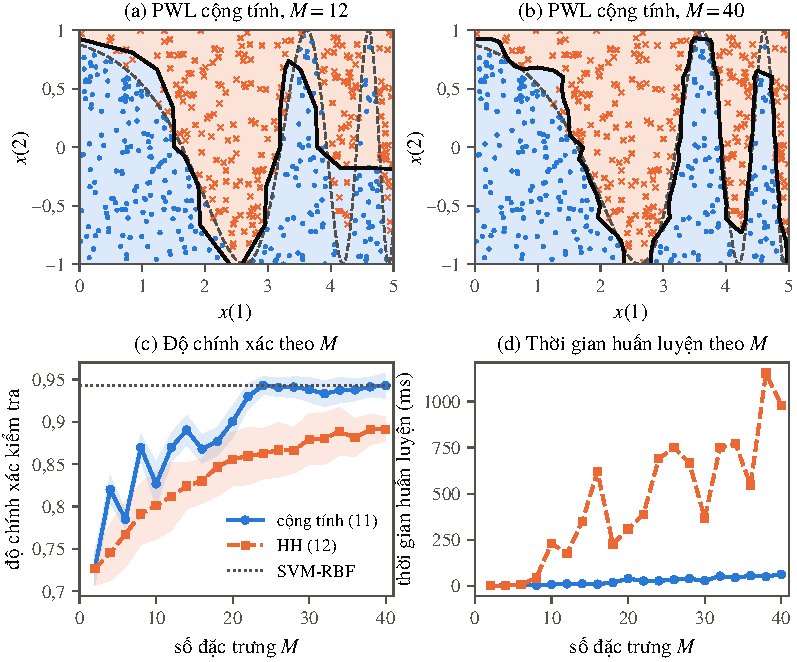
\includegraphics[width=\linewidth]{fig_cosexp_M.pdf}
\caption[Tái hiện thí nghiệm Cosexp: ảnh hưởng của số đặc trưng]{Tái hiện thí nghiệm Cosexp (Hình~3 của~\cite{huang2013}), $10$ lần lặp. (a), (b) Biên của PWL-C-SVM cộng tính với $M=12$ và $M=40$ (nét liền) so với biên thật (nét đứt). (c) Độ chính xác trên tập kiểm tra theo $M$: đường là trung bình, dải màu là $\pm$ một độ lệch chuẩn; đường chấm là SVM hạt nhân Gauss. (d) Thời gian huấn luyện (trung vị) với $\gamma$ đã chọn.}
\label{fig:cosexp}
\end{figure}

\Cref{fig:cosexp} tái hiện đúng xu hướng mà bài báo gốc báo cáo. Với $M=2$, bộ phân loại chỉ là tuyến tính và đạt $72{,}7\pm2{,}0\%$ (bài báo: $76{,}83\%$ với một lần chạy). Khi $M$ tăng, biên uốn theo đường cong thật ngày càng sát (\cref{fig:cosexp}a,b); độ chính xác đạt $90{,}0\%$ tại $M=20=10n$ và ổn định quanh $94\%$ từ $M=24$, ngang với SVM hạt nhân Gauss ($94{,}2\pm0{,}9\%$). Ở $M$ nhỏ, đường cong không đơn điệu: mỗi giá trị của $M$ ứng với một lưới nút hoàn toàn khác, và độ chính xác phụ thuộc vào việc các nút có rơi gần những chỗ biên đổi hướng hay không. Thời gian huấn luyện tăng theo $M$ nhưng vẫn dưới $0{,}1$ giây (\cref{fig:cosexp}d).

Đáng chú ý, trên dữ liệu này ánh xạ HH kém hẳn ánh xạ cộng tính ($89{,}1\pm1{,}4\%$ tại $M=40$), dù về lý thuyết nó linh hoạt hơn. Lý do là nhãn của Cosexp được xác định bởi hàm $\cos\bigl(0{,}5\,e^{0{,}7x(1)}\bigr)-x(2)$, một hàm cộng tính: ánh xạ cộng tính khớp đúng cấu trúc đó, còn các siêu phẳng ngẫu nhiên của HH phân tán khả năng biểu diễn vào những hướng không cần thiết. Kết hợp với Mục~\ref{sec:exp2d}, ta rút ra một quy tắc thực hành: nên thử ánh xạ cộng tính trước, vì nó rẻ, dễ diễn giải và đủ tốt khi tương tác giữa các biến yếu; chỉ chuyển sang HH khi có dấu hiệu tương tác mạnh, như trên bàn cờ. Đây cũng là thứ tự mà bài báo gốc khuyến nghị~\cite[Mục~4]{huang2013}.

% Generated by code/fill_numbers.py from chuong3_bench_b.tpl -- edit the template, not this file.
% ----------------------------------------------------------------------------
\subsection{Mười bộ dữ liệu chuẩn}\label{sec:bench10}

\paragraph{Dữ liệu và giao thức.} Đề án dùng mười bộ dữ liệu phân loại nhị phân (\cref{tab:datasets}). Bảy bộ trong số đó có mặt trong Bảng~1 của bài báo gốc (Haberman, Transfusion, Pima, Breast, Magic, Parkinsons, Ionosphere); ba bộ còn lại (Banknote, Spambase, Sonar) được thêm vào để bao quát thêm các kích thước dữ liệu và số chiều khác nhau. Mỗi bộ được chia ngẫu nhiên có phân tầng thành hai nửa huấn luyện và kiểm tra, lặp lại $10$ lần; với Magic, tập huấn luyện gồm $2.000$ điểm như trong bài báo gốc, phần còn lại dùng để kiểm tra; với Spambase, do chi phí tinh chỉnh các mô hình hạt nhân lớn, chỉ lặp lại $5$ lần. Trên mỗi tập huấn luyện, tham số được chọn bằng kiểm định chéo $10$ phần: $\gamma\in\{2^{-5},2^{-3},\dots,2^{11}\}$ cho mọi mô hình SVM, tham số $1/\sigma^2$ của hạt nhân Gauss trên lưới $\{2^{-15},2^{-13},\dots,2^{3}\}$ theo khuyến nghị của~\cite{hsu2003}, và hệ số phạt $L_2$ của mạng nơ-ron trong $\{10^{-4},10^{-3},\dots,1\}$. Chín phương pháp được so sánh: SVM tuyến tính; SVM và LS-SVM hạt nhân Gauss; kNN với $k=1$ như trong bài báo; Ik-SVM; mạng nơ-ron một lớp ẩn gồm $D=9n$ nơ-ron ReLU, bằng đúng số đặc trưng bản lề của PWL-SVM dạng HH, được huấn luyện bằng L-BFGS~\cite{liu1989}; và ba biến thể PWL-SVM với $M/n=10$ theo đúng quy tắc của bài báo: PWL-C-SVM và PWL-LS-SVM với ánh xạ cộng tính lưới đều, và PWL-C-SVM với ánh xạ HH chuẩn hóa $|p(1)|=1$.

\input{chapters/tab_datasets}

\input{chapters/tab_bench}

\paragraph{Kết quả tổng quát.} \Cref{tab:bench} cho độ chính xác trung bình và \cref{fig:bench-diff} biểu diễn chênh lệch so với SVM hạt nhân Gauss; độ lệch chuẩn và kích thước mô hình được cho ở Phụ lục~B. Ba phương pháp dẫn đầu về độ chính xác là LS-SVM hạt nhân Gauss, mạng nơ-ron và SVM hạt nhân Gauss, với hạng trung bình lần lượt $2{,}35$, $3{,}00$ và $3{,}15$. PWL-C-SVM cộng tính đứng giữa bảng (hạng $5{,}35$), trên SVM tuyến tính ($6{,}55$) và kNN ($7{,}40$).

Bức tranh rõ hơn khi tách các bộ dữ liệu thành hai nhóm. Ở nhóm thứ nhất gồm Haberman, Transfusion, Banknote, Pima và Breast, mọi phương pháp dựa trên SVM, kể cả SVM tuyến tính, chênh nhau không quá khoảng $1{,}5$ điểm phần trăm: một biên tuyến tính đã gần như đủ tốt, và tính phi tuyến không đem lại lợi ích đáng kể. Ở nhóm thứ hai gồm Magic, Parkinsons, Ionosphere, Sonar, nơi SVM tuyến tính kém SVM hạt nhân Gauss từ $4$ đến $9$ điểm, PWL-C-SVM cộng tính thu hẹp đáng kể khoảng cách trên ba trong bốn bộ: nó cải thiện so với SVM tuyến tính $5{,}8$ điểm trên Magic, $3{,}5$ điểm trên Ionosphere và $5{,}0$ điểm trên Sonar, nhưng vẫn kém SVM hạt nhân Gauss từ $0{,}7$ đến $4{,}1$ điểm. Magic là trường hợp đáng chú ý nhất: PWL-C-SVM đạt $84{,}8\%$ so với $85{,}5\%$ của SVM hạt nhân Gauss, trong khi mô hình chỉ gồm $211$ số thực so với $7.694$ số, nhỏ hơn khoảng $36$ lần.

\begin{figure}[t]
\centering
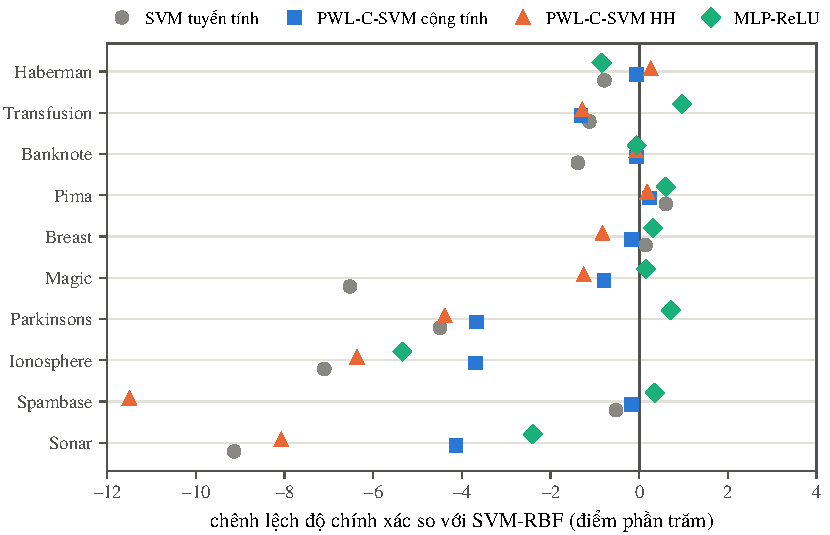
\includegraphics[width=\linewidth]{fig_benchmark_diff.pdf}
\caption[Chênh lệch độ chính xác so với SVM hạt nhân Gauss]{Chênh lệch độ chính xác trung bình so với SVM hạt nhân Gauss (điểm phần trăm; giá trị âm nghĩa là kém hơn) của bốn phương pháp trên mười bộ dữ liệu.}
\label{fig:bench-diff}
\end{figure}

\input{chapters/tab_wilcoxon}

\paragraph{Kiểm định thống kê.} \Cref{tab:wilcoxon} so sánh PWL-C-SVM cộng tính với từng phương pháp bằng kiểm định dấu hạng Wilcoxon trên mười cặp giá trị trung bình, theo khuyến nghị của Demšar~\cite{demsar2006}. Ở mức ý nghĩa $5\%$, PWL-C-SVM cộng tính kém SVM hạt nhân Gauss và LS-SVM hạt nhân Gauss một cách có ý nghĩa ($p=0{,}014$ và $p=0{,}008$). Nó cao hơn SVM tuyến tính trên bảy trong mười bộ, với chênh lệch trung bình $1{,}7$ điểm, và khác biệt này có ý nghĩa thống kê ($p=0{,}037$); khác biệt so với mạng nơ-ron và Ik-SVM không có ý nghĩa thống kê. Với chỉ mười bộ dữ liệu, các kiểm định này có lực thấp, nên “không bác bỏ” không có nghĩa là “tương đương”.

\paragraph{Ánh xạ HH và quy tắc chọn tham số.} PWL-C-SVM với ánh xạ HH có hạng trung bình thấp ($6{,}60$), và trên Spambase kết quả của nó rất bất ổn: ở lần chia đầu tiên, mô hình thất bại hoàn toàn ($40{,}0\%$, thấp hơn cả tỉ lệ $60{,}6\%$ của lớp đa số), trong khi ở bốn lần chia còn lại nó đạt từ $91{,}0\%$ đến $93{,}7\%$. Nguyên nhân nằm ở quy tắc sinh tham số chứ không ở mô hình. Dữ liệu Spambase rất thưa: sau khi chuẩn hóa, gần $78\%$ các giá trị bằng $0$, và phần lớn dữ liệu nằm sát một đỉnh của hình hộp $[0,1]^{57}$. Các siêu phẳng đi qua những điểm lấy đều trong hình hộp vì vậy thường không cắt qua vùng dữ liệu: ở mỗi lần chia, từ 18\% đến 22\% số đặc trưng bản lề bằng $0$ trên mọi điểm huấn luyện, và từ 17\% đến 22\% luôn hoạt động, tức là chỉ tuyến tính trên dữ liệu. Nghiêm trọng hơn, việc cố định $|p(1)|=1$ (\cref{rem:scale}) làm độ lớn của các đặc trưng phụ thuộc mạnh vào lần sinh ngẫu nhiên: giá trị lớn nhất của các đặc trưng trên tập huấn luyện dao động từ $423$ đến $3{,}3\cdot10^{5}$ giữa các lần chia. Ở lần chia đầu tiên, một siêu phẳng gần song song với trục $x(1)$ có hệ số lên tới $5{,}3\cdot10^{4}$, khiến bài toán tối ưu bị điều kiện hóa rất kém và bộ giải LIBLINEAR không hội tụ tới một nghiệm có ý nghĩa. Chỉ cần chuẩn hóa $\|p\|_2=1$, các đặc trưng trên dữ liệu huấn luyện không vượt quá $2{,}0$ ở mọi lần chia, và với cùng giao thức, PWL-C-SVM HH đạt $93{,}4\pm0{,}2\%$ trên Spambase. Nhìn chung, mạng nơ-ron với cùng số nơ-ron ẩn tốt hơn PWL-C-SVM HH trên tám trong mười bộ: học lớp ẩn từ dữ liệu có lợi hơn nhiều so với sinh nó ngẫu nhiên, và đó là cái giá của tính lồi đã được nêu ở Mục~\ref{sec:pwlsvm}.

\paragraph{So với bài báo gốc.} Kết quả trên không xác nhận nhận định của bài báo gốc rằng PWL-SVM có độ chính xác tương đương SVM hạt nhân Gauss~\cite{huang2013}. Nguyên nhân chính là bài báo chỉ dùng một lần chia dữ liệu: trên các bộ nhỏ như Parkinsons, với $98$ điểm kiểm tra, độ lệch chuẩn giữa các lần chia lên tới $2$--$4$ điểm phần trăm, nên một lần chia có thể cho kết quả rất lạc quan; bài báo báo cáo độ chính xác $100\%$ cho PWL-C-SVM trên bộ này, trong khi trung bình qua mười lần chia là $86{,}2\%$. Mặt khác, lợi thế về kích thước mô hình được xác nhận rõ ràng: với ánh xạ cộng tính, PWL-C-SVM cần từ $64$ đến $1.261$ số thực, nhỏ hơn SVM hạt nhân Gauss từ $2{,}5$ đến $36$ lần trên cả mười bộ dữ liệu (Phụ lục~B).

% ----------------------------------------------------------------------------
\subsection{Ảnh hưởng của số đặc trưng và của quy tắc chọn tham số}\label{sec:sensitivity}

Để trả lời câu hỏi CH3 một cách có kiểm soát, ta cố định mô hình là PWL-LS-SVM, giải chính xác bằng hồi quy ridge (\cref{prop:ridge}) để loại trừ ảnh hưởng của bộ giải, và thay đổi hai yếu tố: số đặc trưng trên mỗi chiều $M/n\in\{1,2,3,5,10,20\}$ và quy tắc chọn tham số. Bốn quy tắc được so sánh: ánh xạ cộng tính với lưới đều (quy tắc của bài báo gốc) và với lưới phân vị (\cref{rem:quantile}); ánh xạ HH với $|p(1)|=1$ (quy tắc của bài báo gốc) và với $\|p\|_2=1$ (\cref{rem:scale}). Thí nghiệm được thực hiện trên ba bộ dữ liệu có đặc điểm khác nhau --- Ionosphere ($n=33$), Magic ($n=10$, nhiều dữ liệu) và Spambase ($n=57$, rất thưa) --- với $5$ lần chia như ở Mục~\ref{sec:bench10} và $\gamma$ chọn bằng kiểm định chéo $5$ phần. Kết quả được vẽ ở \cref{fig:sensitivity}.

\begin{figure}[t]
\centering
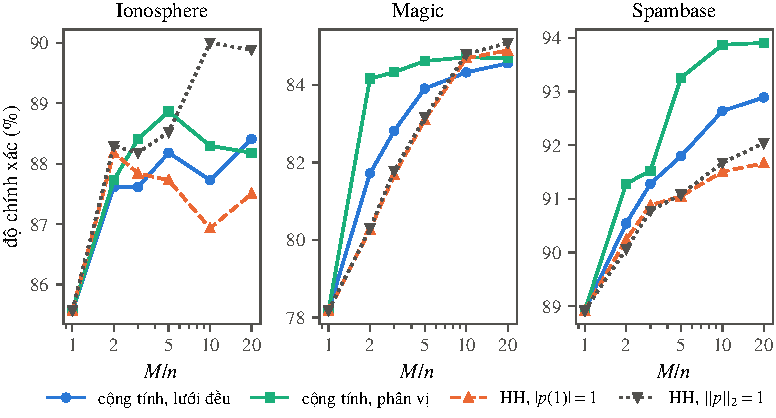
\includegraphics[width=\linewidth]{fig_sensitivity.pdf}
\caption[Ảnh hưởng của số đặc trưng và quy tắc chọn tham số]{Độ chính xác trung bình (qua $5$ lần chia) của PWL-LS-SVM theo số đặc trưng trên mỗi chiều $M/n$, với bốn quy tắc chọn tham số. $M/n=1$ ứng với bộ phân loại tuyến tính.}
\label{fig:sensitivity}
\end{figure}

Có bốn nhận xét. Thứ nhất, độ chính xác tăng nhanh khi $M/n$ tăng từ $1$ (bộ phân loại tuyến tính) và bão hòa quanh $M/n=5$--$10$, phù hợp với quy tắc $M=10n$ của bài báo gốc; tăng tiếp lên $M/n=20$ hầu như không có lợi. Thứ hai, đặt nút theo phân vị cho kết quả tốt hơn hoặc ngang lưới đều trên cả ba bộ dữ liệu, và khác biệt rõ nhất trên những dữ liệu có phân bố lệch: trên Magic, lưới phân vị đạt $84{,}2\%$ ngay với $M/n=2$, trong khi lưới đều cần $M/n=10$ để đạt $84{,}3\%$; trên Spambase, lưới phân vị đạt $93{,}9\%$ so với $92{,}6\%$ của lưới đều ở $M/n=10$, đồng thời chỉ dùng $156$ đặc trưng thay vì $570$, vì các nút trùng nhau của những biến gần như luôn bằng $0$ bị loại bỏ. Thứ ba, ánh xạ HH cần nhiều đặc trưng hơn hẳn mới đạt tới độ chính xác của ánh xạ cộng tính: trên Magic, nó chỉ đuổi kịp lưới phân vị khi $M/n\ge10$ (và nhỉnh hơn $0{,}4$ điểm ở $M/n=20$), còn trên Spambase nó kém ở mọi giá trị của $M/n$; chỉ trên Ionosphere, nơi tương tác giữa các biến có vai trò, HH với $\|p\|_2=1$ đạt kết quả tốt nhất ($90{,}0\%$ ở $M/n=10$). Thứ tư, chuẩn hóa $\|p\|_2=1$ không bao giờ làm kết quả xấu đi đáng kể và cải thiện rõ trên Ionosphere ($90{,}0\%$ so với $86{,}9\%$ ở $M/n=10$); kết hợp với sự cố của LIBLINEAR trên Spambase, đây là một lý do mạnh để thay quy tắc $|p(1)|=1$ bằng $\|p\|_2=1$.

Từ đó rút ra một quy trình thực hành cho dữ liệu dạng bảng: bắt đầu với ánh xạ cộng tính, nút theo phân vị và $M/n$ khoảng $5$ đến $10$; chỉ dùng ánh xạ HH, với các siêu phẳng được chuẩn hóa, khi có dấu hiệu tương tác mạnh giữa các biến. Quy trình này được áp dụng cho bài toán tín dụng ở Mục~\ref{sec:application}.


% Generated by code/fill_numbers.py from chuong3_cost.tpl -- edit the template, not this file.
% ----------------------------------------------------------------------------
\section{Chi phí tính toán và bộ nhớ}\label{sec:cost}

Mục~\ref{sec:pwlsvm} dự báo rằng lợi thế của PWL-SVM nằm ở khâu dự đoán: mô hình chỉ gồm $w$, $w_0$ và tham số của ánh xạ, và việc dự đoán chỉ gồm các phép so sánh, nhân, cộng và lấy cực đại (\cref{tab:cost}). Mục này kiểm tra dự báo đó trên hai bộ dữ liệu lớn hơn: Magic với $9.510$ mẫu huấn luyện (chia đôi toàn bộ dữ liệu) và dữ liệu tín dụng sẽ được mô tả ở Mục~\ref{sec:application}, với $21.000$ mẫu huấn luyện. Để phép đo công bằng, mọi mô hình chạy trên một luồng xử lý của cùng một máy tính, khi không có tiến trình nặng nào khác; tham số được chọn trước bằng kiểm định chéo trên một mẫu con $4.000$ điểm, và chỉ thời gian của một lần huấn luyện với tham số đã chọn được đo. Thời gian dự đoán là trung vị của bảy lần dự đoán toàn bộ tập kiểm tra, chia cho số mẫu. PWL-SVM dùng ánh xạ cộng tính với nút phân vị và $M/n=10$, theo quy trình rút ra ở Mục~\ref{sec:sensitivity}; thẻ điểm là hồi quy logistic trên các biến rời rạc hóa, như ở Mục~\ref{sec:application}.


\paragraph{Dự đoán và bộ nhớ.} Kết quả ở \cref{tab:cost-measured} và \cref{fig:cost} xác nhận dự báo lý thuyết. PWL-LS-SVM cộng tính dự đoán mỗi mẫu trong $0{,}33$~$\mu$s trên Magic và $0{,}56$~$\mu$s trên dữ liệu tín dụng, nhanh hơn SVM hạt nhân Gauss khoảng 200 và 430 lần. Chênh lệch đến từ cấu trúc của mô hình: trên dữ liệu tín dụng, SVM hạt nhân Gauss lưu $239.111$ số thực, ứng với khoảng $8.854$ vectơ hỗ trợ, và mỗi lần dự đoán phải tính chừng ấy khoảng cách cùng hàm mũ; còn PWL-SVM cộng tính chỉ lưu $349$ số và thực hiện vài trăm phép so sánh, nhân và cộng, đúng như các công thức ở \cref{tab:cost}. Trên dữ liệu tín dụng, mạng nơ-ron dự đoán nhanh ngang PWL-SVM cộng tính, còn tổ hợp cây tăng cường chậm hơn khoảng 2{,}5 lần; cả hai mô hình cũng lớn hơn nhiều, với $6.605$ và khoảng $4.514$ số thực. Thẻ điểm có kích thước tương đương PWL-SVM cộng tính ($379$ so với $349$ số thực), và trong cài đặt dựa trên scikit-learn, nó dự đoán chậm hơn PWL-SVM khoảng 2{,}6 lần. Chỉ các mô hình tuyến tính trên biến gốc là nhỏ và nhanh hơn PWL-SVM, với cái giá là độ chính xác thấp hơn rõ rệt: trên Magic, hồi quy logistic đạt $78{,}7\%$ so với $84{,}8\%$ của PWL-LS-SVM cộng tính.

\begin{table}[t]
\centering
\caption[Chi phí huấn luyện, dự đoán và bộ nhớ]{Chi phí trên Magic ($9.510$ mẫu huấn luyện) và dữ liệu tín dụng ($21.000$ mẫu huấn luyện), đo trên một luồng xử lý: thời gian huấn luyện một mô hình với tham số đã chọn, thời gian dự đoán mỗi mẫu, số thực cần lưu, và độ chính xác (Magic) hoặc AUC (tín dụng) trên tập kiểm tra. Đây là một lần chia riêng, với tham số chọn trên mẫu con (và với Magic, tập huấn luyện lớn hơn nhiều), nên độ chính xác khác với ở \cref{tab:bench,tab:credit}.}
\label{tab:cost-measured}
\footnotesize
\setlength{\tabcolsep}{3pt}
\renewcommand{\arraystretch}{1.18}
\begin{tabular}{@{}l r r r c r r r c@{}}
\toprule
 & \multicolumn{4}{c}{\textbf{Magic}} & \multicolumn{4}{c}{\textbf{Tín dụng}}\\
\cmidrule(lr){2-5}\cmidrule(l){6-9}
\textbf{Mô hình} & \begin{tabular}[b]{@{}c@{}}\textbf{Huấn}\\\textbf{luyện (s)}\end{tabular} & \begin{tabular}[b]{@{}c@{}}\textbf{Dự đoán}\\\textbf{($\mu$s/mẫu)}\end{tabular} & \begin{tabular}[b]{@{}c@{}}\textbf{Số}\\\textbf{thực}\end{tabular} & \begin{tabular}[b]{@{}c@{}}\textbf{ĐCX}\\\textbf{(\%)}\end{tabular} & \begin{tabular}[b]{@{}c@{}}\textbf{Huấn}\\\textbf{luyện (s)}\end{tabular} & \begin{tabular}[b]{@{}c@{}}\textbf{Dự đoán}\\\textbf{($\mu$s/mẫu)}\end{tabular} & \begin{tabular}[b]{@{}c@{}}\textbf{Số}\\\textbf{thực}\end{tabular} & \textbf{AUC}\\
\midrule
SVM tuyến tính & 5{,}2 & 0{,}02 & 31 & 78{,}7 & 9{,}3 & 0{,}06 & 79 & 0{,}694\\
Hồi quy logistic & 0{,}00 & 0{,}02 & 31 & 78{,}7 & 0{,}02 & 0{,}05 & 79 & 0{,}716\\
Thẻ điểm & 0{,}02 & 0{,}69 & 191 & 84{,}6 & 0{,}07 & 1{,}4 & 379 & 0{,}768\\
PWL-C-SVM, cộng tính & 4{,}7 & 0{,}33 & 211 & 85{,}7 & 52 & 0{,}58 & 349 & 0{,}685\\
PWL-LS-SVM, cộng tính & 0{,}01 & 0{,}33 & 211 & 84{,}8 & 0{,}04 & 0{,}56 & 349 & 0{,}768\\
PWL-LS-SVM, HH & 0{,}01 & 0{,}40 & 1.111 & 85{,}1 & 0{,}07 & 1{,}3 & 6.631 & 0{,}740\\
SVM-RBF & 0{,}76 & 64{,}7 & 34.462 & 87{,}1 & 4{,}6 & 241 & 239.111 & 0{,}711\\
MLP-ReLU & 2{,}9 & 0{,}18 & 1.101 & 86{,}5 & 21 & 0{,}57 & 6.605 & 0{,}761\\
Tổ hợp cây tăng cường & 0{,}11 & 3{,}8 & 12.200 & 88{,}1 & 0{,}15 & 1{,}4 & 4.514 & 0{,}774\\
\bottomrule
\end{tabular}
\end{table}


\begin{figure}[t]
\centering
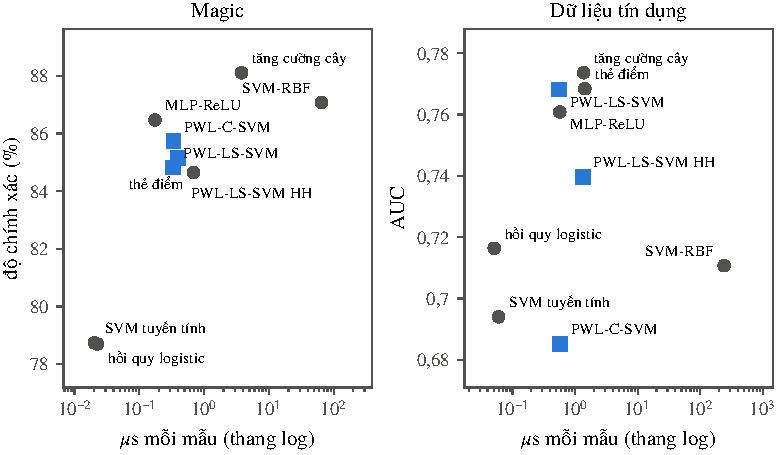
\includegraphics[width=\linewidth]{fig_cost.pdf}
\caption[Đánh đổi giữa độ chính xác và thời gian dự đoán]{Độ chính xác (Magic) hoặc AUC (dữ liệu tín dụng) theo thời gian dự đoán mỗi mẫu, trên thang logarit. Ô vuông là các biến thể PWL-SVM; điểm tròn là các phương pháp khác.}
\label{fig:cost}
\end{figure}

\paragraph{Huấn luyện.} PWL-LS-SVM là mô hình phi tuyến huấn luyện nhanh nhất: $0{,}01$ giây trên Magic và $0{,}04$ giây trên dữ liệu tín dụng, vì chỉ cần lập và giải một hệ tuyến tính cỡ $M\times M$ (\cref{prop:ridge}). PWL-C-SVM chậm hơn ($4{,}7$ và $52$ giây) vì bộ giải lặp của LIBLINEAR cần nhiều vòng để hội tụ. SVM hạt nhân Gauss cần $0{,}76$ và $4{,}6$ giây, và chi phí này tăng nhanh hơn tuyến tính theo số mẫu~\cite{chang2011}; mạng nơ-ron cần $2{,}9$ và $21$ giây. Trong một quy trình thực tế, nơi mô hình phải được huấn luyện lại nhiều lần để chọn tham số, khác biệt này còn được nhân lên theo kích thước lưới tham số.

Cần lưu ý rằng số đo tuyệt đối phụ thuộc vào cài đặt: PWL-SVM được cài bằng NumPy, còn LIBSVM là thư viện C đã được tối ưu nhiều năm. Trên một thiết bị nhúng, số phép tính và số thực cần lưu ở \cref{tab:cost} mới là thước đo phù hợp, và ở cả hai thước đo đó, PWL-SVM cộng tính có lợi thế lớn so với SVM hạt nhân Gauss.

% ----------------------------------------------------------------------------
\section{Ứng dụng: dự báo vỡ nợ thẻ tín dụng}\label{sec:application}

\subsection{Bài toán và dữ liệu}

Ngân hàng phát hành thẻ tín dụng cần ước lượng khả năng một khách hàng không thanh toán được dư nợ trong kỳ tới, để điều chỉnh hạn mức, ưu tiên nhắc nợ hoặc trích lập dự phòng rủi ro. Đây là một bài toán phân loại nhị phân điển hình của chấm điểm tín dụng~\cite{thomas2002}, và cả ba yêu cầu nêu ở Mở đầu đều có mặt: độ chính xác quyết định trực tiếp chi phí rủi ro; số hồ sơ lớn và việc chấm điểm được lặp lại định kỳ, nên chi phí dự đoán đáng kể; và tổ chức tín dụng cần giải thích được quyết định của mình với khách hàng cũng như với cơ quan quản lý.

Đề án dùng dữ liệu của Yeh và Lien~\cite{yeh2009} về $30.000$ chủ thẻ tín dụng của một ngân hàng ở Đài Loan, trong giai đoạn từ tháng 4 đến tháng 9 năm 2005. Nhãn cho biết khách hàng có vỡ nợ trong tháng tiếp theo hay không; có $6.636$ khách hàng vỡ nợ, tức $22{,}1\%$. Hai mươi ba biến giải thích thuộc bốn nhóm: hạn mức tín dụng, thông tin nhân khẩu học, lịch sử trả nợ sáu tháng gần nhất và các số tiền sao kê, thanh toán tương ứng (\cref{tab:credit-vars}).

\begin{table}[t]
\centering
\caption[Các biến của dữ liệu vỡ nợ thẻ tín dụng]{Các biến của dữ liệu vỡ nợ thẻ tín dụng~\cite{yeh2009} và cách xử lý trong đề án. Số tiền tính bằng Đài tệ.}
\label{tab:credit-vars}
\small
\renewcommand{\arraystretch}{1.2}
\begin{tabularx}{\linewidth}{@{}l X X@{}}
\toprule
\textbf{Biến} & \textbf{Ý nghĩa} & \textbf{Xử lý}\\
\midrule
LIMIT\_BAL & hạn mức tín dụng của khách hàng và gia đình & giữ nguyên\\
SEX & giới tính (1 nam, 2 nữ) & một biến chỉ báo “nữ”\\
EDUCATION & học vấn (1 sau đại học, 2 đại học, 3 trung học, 4 khác) & ba biến chỉ báo; các mã $0,5,6$ không được mô tả, gộp vào “khác”\\
MARRIAGE & hôn nhân (1 đã kết hôn, 2 độc thân, 3 khác) & hai biến chỉ báo; mã $0$ gộp vào “khác”\\
AGE & tuổi & giữ nguyên\\
PAY\_0, PAY\_2, \dots, PAY\_6 & trạng thái trả nợ các tháng 9, 8, \dots, 4: $-1$ trả đúng hạn, $k\ge1$ chậm $k$ tháng; các mã $-2$ và $0$ cũng xuất hiện & giữ nguyên như biến thứ bậc\\
BILL\_AMT1, \dots, BILL\_AMT6 & dư nợ sao kê các tháng 9, \dots, 4 & giữ nguyên\\
PAY\_AMT1, \dots, PAY\_AMT6 & số tiền đã thanh toán các tháng 9, \dots, 4 & giữ nguyên\\
\bottomrule
\end{tabularx}
\end{table}

Sau khi mã hóa các biến định danh, mỗi khách hàng được mô tả bởi $n=26$ đặc trưng số. Hai đặc điểm của dữ liệu quyết định thiết kế mô hình (\cref{fig:credit-overview}). Thứ nhất, quan hệ giữa lịch sử trả nợ và rủi ro là phi tuyến rõ rệt: tỉ lệ vỡ nợ gần như không đổi, khoảng $13$--$17\%$, với các trạng thái $-2$, $-1$ và $0$, rồi tăng vọt lên $34\%$ khi chậm một tháng và gần $70\%$ khi chậm hai tháng. Một mô hình tuyến tính theo PAY\_0 không thể mô tả bước nhảy này, trong khi một hàm tuyến tính từng phần với vài điểm gãy thì có thể. Thứ hai, các biến tiền tệ lệch rất mạnh: hạn mức trải từ $10$ nghìn đến $1$ triệu Đài tệ, nhưng một nửa số khách hàng có hạn mức không vượt quá $140$ nghìn. Lưới nút đều của bài báo gốc vì vậy đặt phần lớn các nút ở vùng gần như không có dữ liệu, còn lưới theo phân vị (\cref{rem:quantile}) đặt nút theo mật độ dữ liệu.

\begin{figure}[t]
\centering
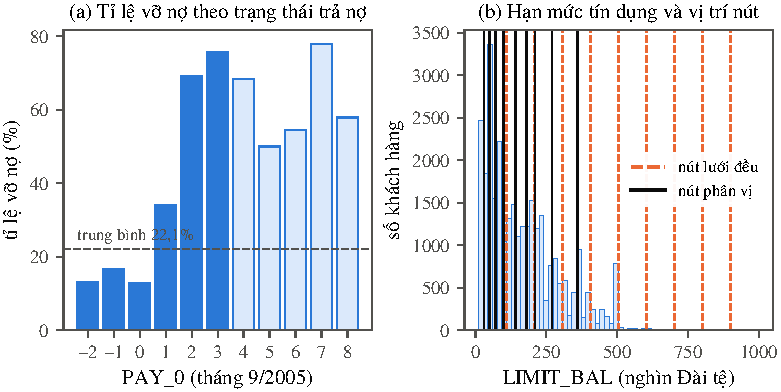
\includegraphics[width=\linewidth]{fig_credit_overview.pdf}
\caption[Hai đặc điểm của dữ liệu tín dụng]{(a) Tỉ lệ vỡ nợ theo trạng thái trả nợ tháng 9 (PAY\_0); cột nhạt ứng với các nhóm có ít hơn $100$ khách hàng. (b) Phân bố hạn mức tín dụng cùng vị trí $9$ nút của lưới đều (nét đứt) và của lưới theo phân vị (nét liền).}
\label{fig:credit-overview}
\end{figure}

\subsection{Thiết kế thực nghiệm}

Dữ liệu được chia ngẫu nhiên có phân tầng theo tỉ lệ $70/30$, thành $21.000$ khách hàng huấn luyện và $9.000$ khách hàng kiểm tra, lặp lại $5$ lần. Độ đo chính là diện tích dưới đường cong ROC (AUC)~\cite{fawcett2006}: xác suất để một khách hàng vỡ nợ chọn ngẫu nhiên được mô hình chấm điểm rủi ro cao hơn một khách hàng không vỡ nợ chọn ngẫu nhiên. AUC không phụ thuộc vào ngưỡng quyết định và là độ đo chuẩn trong chấm điểm tín dụng~\cite{lessmann2015}. Để đánh giá thêm chất lượng phân loại, đề án chọn một ngưỡng trên tập huấn luyện sao cho tỉ lệ khách hàng bị dự báo vỡ nợ bằng tỉ lệ vỡ nợ quan sát được, rồi tính độ chính xác cân bằng (trung bình của độ nhạy và độ đặc hiệu) và độ đo F1 của lớp vỡ nợ trên tập kiểm tra. Quy tắc chọn ngưỡng này tương ứng với chính sách “đưa vào diện theo dõi một tỉ lệ khách hàng cố định”.

Mười mô hình được so sánh. Ba mô hình tuyến tính đóng vai trò chuẩn so sánh của ngành: hồi quy logistic trên các biến gốc, SVM tuyến tính, và \emph{thẻ điểm} --- hồi quy logistic trên các biến đã được rời rạc hóa, theo cách xây dựng thẻ điểm truyền thống~\cite{thomas2002}, trong đó mỗi biến liên tục được chia thành mười khoảng theo thập phân vị và mỗi giá trị của các biến PAY là một hạng mục riêng. Bốn biến thể PWL-SVM được thử: PWL-LS-SVM cộng tính với lưới đều (quy tắc của bài báo gốc) và với lưới phân vị, PWL-C-SVM cộng tính với lưới phân vị, và PWL-LS-SVM với ánh xạ HH; mọi biến thể dùng $M/n=10$. Ba mô hình phi tuyến làm đối chứng: SVM hạt nhân Gauss, mạng nơ-ron một lớp ẩn với $9n=234$ nơ-ron ReLU, huấn luyện bằng L-BFGS~\cite{liu1989}, và tổ hợp cây tăng cường~\cite{friedman2001} với thiết lập mặc định của scikit-learn, là một đại diện cho nhóm mô hình thường chính xác nhất trên dữ liệu dạng bảng~\cite{lessmann2015}. Tham số của mỗi mô hình được chọn bằng kiểm định chéo $5$ phần trên tập huấn luyện với tiêu chí AUC; riêng SVM hạt nhân Gauss và mạng nơ-ron được tinh chỉnh trên một mẫu con phân tầng gồm $5.000$ và $7.000$ khách hàng với kiểm định chéo $3$ phần, rồi huấn luyện lại trên toàn bộ tập huấn luyện, vì chi phí huấn luyện của chúng lớn hơn nhiều. Các lưới tham số là: $\gamma\in\{2^{-9},2^{-7},\dots,2^{7}\}$ cho SVM tuyến tính và mọi biến thể PWL-SVM; $\gamma\in\{2^{-2},2^{0},2^{2},2^{4}\}$ và $1/\sigma^2\in\{2^{-7},2^{-5},2^{-3},2^{-1}\}$ cho SVM hạt nhân Gauss; hệ số phạt $L_2$ trong $\{10^{-2},10^{-1},1,10\}$ cho mạng nơ-ron; nghịch đảo của hệ số phạt trong $\{10^{-3},10^{-2},\dots,10\}$ cho hồi quy logistic và thẻ điểm. Tổ hợp cây tăng cường dùng thiết lập mặc định, có cơ chế dừng sớm trên một phần dữ liệu kiểm định nội bộ.


% Generated by code/fill_numbers.py from chuong3_credit_b.tpl -- edit the template, not this file.
\subsection{Kết quả}\label{sec:credit-results}

\begin{table}[t]
\centering
\caption[Kết quả trên dữ liệu vỡ nợ thẻ tín dụng]{Kết quả trên dữ liệu vỡ nợ thẻ tín dụng (trung bình $\pm$ độ lệch chuẩn qua $5$ lần chia $70/30$). AUC: diện tích dưới đường ROC; ĐCX-CB: độ chính xác cân bằng; F1 tính cho lớp vỡ nợ; ngưỡng được chọn trên tập huấn luyện sao cho tỉ lệ dự báo vỡ nợ bằng tỉ lệ vỡ nợ quan sát. Cột cuối: số thực cần lưu (trung vị); thời gian dự đoán được đo riêng ở \cref{sec:cost}.}
\label{tab:credit}
\footnotesize
\setlength{\tabcolsep}{3pt}
\renewcommand{\arraystretch}{1.18}
\begin{tabular}{@{}l c c c r@{}}
\toprule
\textbf{Mô hình} & \textbf{AUC} & \textbf{ĐCX-CB (\%)} & \textbf{F1 (\%)} & \textbf{Số thực}\\
\midrule
Hồi quy logistic & $0{,}724\pm0{,}009$ & $68{,}7\pm0{,}6$ & $51{,}2\pm0{,}9$ & 79\\
Thẻ điểm (logistic, biến rời rạc hóa) & $0{,}773\pm0{,}006$ & $70{,}3\pm0{,}6$ & $53{,}7\pm1{,}0$ & 381\\
SVM tuyến tính & $0{,}706\pm0{,}008$ & $68{,}5\pm0{,}8$ & $50{,}9\pm1{,}4$ & 79\\
\midrule
PWL-LS-SVM, cộng tính, lưới đều & $0{,}772\pm0{,}006$ & $70{,}3\pm0{,}5$ & $53{,}6\pm0{,}9$ & 547\\
PWL-LS-SVM, cộng tính, phân vị & $0{,}776\pm0{,}006$ & $70{,}4\pm0{,}7$ & $53{,}8\pm1{,}1$ & 349\\
\quad và ràng buộc đơn điệu (Mục~\ref{sec:monotone}) & $0{,}775\pm0{,}006$ & $70{,}3\pm0{,}8$ & $53{,}7\pm1{,}2$ & 349\\
PWL-C-SVM, cộng tính, phân vị & $0{,}744\pm0{,}007$ & $67{,}8\pm0{,}8$ & $49{,}9\pm1{,}4$ & 349\\
PWL-LS-SVM, HH & $0{,}743\pm0{,}007$ & $69{,}5\pm0{,}6$ & $52{,}4\pm1{,}0$ & 6.631\\
\midrule
SVM-RBF & $0{,}716\pm0{,}010$ & $69{,}2\pm0{,}6$ & $52{,}0\pm1{,}0$ & 243.134\\
MLP-ReLU & $0{,}768\pm0{,}005$ & $70{,}0\pm0{,}4$ & $53{,}3\pm0{,}7$ & 6.605\\
Tổ hợp cây tăng cường & $0{,}779\pm0{,}006$ & $70{,}3\pm0{,}7$ & $53{,}7\pm1{,}1$ & 4.636\\
\bottomrule
\end{tabular}
\end{table}


\begin{figure}[t]
\centering
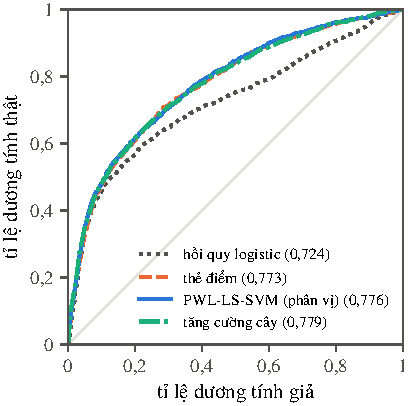
\includegraphics[width=0.62\linewidth]{fig_credit_roc.pdf}
\caption[Đường cong ROC trên dữ liệu tín dụng]{Đường cong ROC trên tập kiểm tra của lần chia đầu tiên cho bốn mô hình; con số trong ngoặc là AUC trung bình qua năm lần chia.}
\label{fig:credit-roc}
\end{figure}

\Cref{tab:credit} và \cref{fig:credit-roc} cho thấy các mô hình chia thành hai nhóm rõ rệt. Nhóm dẫn đầu gồm tổ hợp cây tăng cường (AUC trung bình 0{,}779), PWL-LS-SVM cộng tính với nút phân vị (0{,}776), thẻ điểm logistic trên các biến đã rời rạc hóa (0{,}773) và PWL-LS-SVM cộng tính với lưới đều (0{,}772). Nhóm còn lại gồm hồi quy logistic trên các biến gốc (0{,}724), SVM tuyến tính (0{,}706) và SVM hạt nhân Gauss (0{,}716); mạng nơ-ron (0{,}768) đứng giữa hai nhóm. Như vậy, AUC của PWL-LS-SVM cộng tính với nút phân vị chỉ kém tổ hợp cây tăng cường một chút. Độ chính xác cân bằng và độ đo F1 ở ngưỡng đã chọn dẫn tới cùng kết luận: bốn mô hình của nhóm dẫn đầu gần như ngang nhau và cao hơn rõ rệt hồi quy logistic, SVM tuyến tính và SVM hạt nhân Gauss. Kết quả rất ổn định giữa các lần chia: độ lệch chuẩn của AUC chỉ khoảng 0{,}006.

Khoảng cách 0{,}052 đơn vị AUC giữa PWL-LS-SVM và hồi quy logistic trên các biến gốc cần được hiểu đúng. Phần lớn khoảng cách đó đến từ quan hệ phi tuyến giữa các trạng thái trả nợ và rủi ro (\cref{fig:credit-overview}a), mà một mô hình tuyến tính theo PAY\_0 không mô tả được. Trong thực tế, các thẻ điểm không dùng trực tiếp biến gốc mà rời rạc hóa từng biến thành các khoảng rồi mới hồi quy logistic~\cite{thomas2002}, và thẻ điểm xây dựng theo cách đó ở \cref{tab:credit} đã thu hẹp phần lớn khoảng cách. Thẻ điểm cũng là đối chứng công bằng nhất cho PWL-SVM cộng tính: cả hai đều là mô hình cộng tính, đều dựa trên các khoảng của từng biến, chỉ khác ở chỗ đóng góp của mỗi biến là hàm bậc thang trong thẻ điểm và là đường gấp khúc liên tục trong PWL-SVM. So với thẻ điểm, PWL-LS-SVM cao hơn ở bốn trong năm lần chia, với chênh lệch trung bình 0{,}002 đơn vị AUC, trong khi hai mô hình có kích thước tương đương (349 và 381 số thực). Chênh lệch này nhỏ, nhưng trong chấm điểm tín dụng, ngay cả những cải thiện nhỏ về khả năng phân biệt cũng có thể mang lại lợi ích kinh tế đáng kể khi áp dụng cho một danh mục lớn~\cite{lessmann2015}.

Ba quan sát khác đáng chú ý. Thứ nhất, lưới phân vị tốt hơn lưới đều (0{,}776 so với 0{,}772) với mô hình nhỏ hơn (349 so với 547 số thực), đúng như phân tích ở \cref{fig:credit-overview}b. Thứ hai, với cùng ánh xạ, PWL-C-SVM cho AUC thấp hơn hẳn PWL-LS-SVM (0{,}744). Điều này có thể giải thích bằng hàm mất mát: mất mát bản lề chỉ quan tâm đến các điểm nằm gần hoặc vi phạm lề, nên giá trị hàm quyết định ở xa biên không mang nhiều thông tin về mức độ rủi ro; còn mất mát bình phương của LS-SVM, tương đương hồi quy trên nhãn $\pm1$ (\cref{prop:ridge}), buộc điểm số của mọi khách hàng phải phản ánh nhãn của họ, và vì thế cho một thứ hạng tốt hơn. SVM hạt nhân Gauss, cũng dùng mất mát bản lề, gặp cùng hạn chế. Thứ ba, ánh xạ HH (0{,}743) kém ánh xạ cộng tính: trên dữ liệu này, ảnh hưởng của từng biến quan trọng hơn tương tác giữa các biến, và các siêu phẳng ngẫu nhiên lãng phí khả năng biểu diễn, phù hợp với kết luận của Mục~\ref{sec:sensitivity}.

\subsection{Diễn giải mô hình}\label{sec:credit-interp}

Vì ánh xạ là cộng tính, hàm quyết định của PWL-LS-SVM tách thành tổng các đóng góp của từng biến,
\begin{equation}\label{eq:additive-decomp}
f(x)=w_0+\sum_{i=1}^{n}h_i\bigl(x(i)\bigr),
\end{equation}
trong đó mỗi $h_i$ là một hàm tuyến tính từng phần một biến, có không quá chín điểm gãy đặt tại các phân vị của biến đó (\cref{prop:1d}). Mỗi $h_i$ có thể được vẽ ra và đọc trực tiếp, giống như một thẻ điểm trong đó số điểm cộng thêm cho mỗi khách hàng là một đường gấp khúc theo giá trị của biến. \Cref{fig:credit-shapes} vẽ sáu hàm $h_i$ có ảnh hưởng lớn nhất của mô hình huấn luyện trên lần chia đầu tiên, sau khi trừ đi giá trị trung bình trên tập huấn luyện; giá trị dương nghĩa là rủi ro cao hơn một khách hàng trung bình.

\begin{figure}[t]
\centering
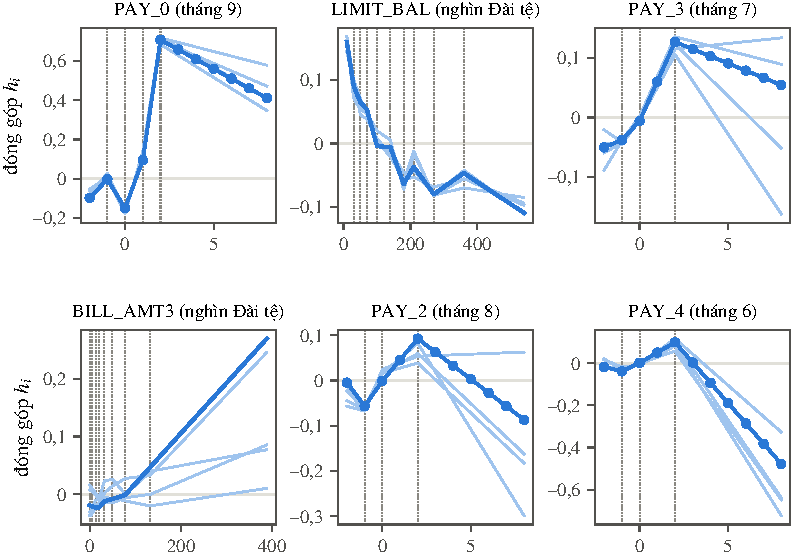
\includegraphics[width=\linewidth]{fig_credit_shapes.pdf}
\caption[Các hàm đóng góp của mô hình PWL-SVM cộng tính]{Sáu hàm đóng góp $h_i$ có ảnh hưởng lớn nhất của PWL-LS-SVM cộng tính (nút phân vị) trên dữ liệu tín dụng, đã trừ giá trị trung bình. Nét đậm: mô hình của lần chia đầu tiên, nét chấm dọc là vị trí các nút của nó; nét mảnh: mô hình của bốn lần chia còn lại. Giá trị dương ứng với rủi ro vỡ nợ cao hơn.}
\label{fig:credit-shapes}
\end{figure}

Hàm đóng góp của PAY\_0 thể hiện rõ cấu trúc mà hồi quy logistic trên biến gốc bỏ lỡ (so sánh với \cref{fig:credit-overview}a). Ba mã không chậm trả ($-2$, $-1$ và $0$) có đóng góp thấp và gần nhau; mã $-1$ cao hơn hai mã còn lại một chút, đúng như tỉ lệ vỡ nợ quan sát được (16{,}8\% so với 13{,}2\% và 12{,}8\%). Đóng góp tăng mạnh khi khách hàng chậm trả một tháng (tỉ lệ vỡ nợ 33{,}9\%) và đạt cực đại khi chậm hai tháng (69{,}1\%); chênh lệch giữa mã $0$ và mã $2$ là $0{,}86$ đơn vị điểm, lớn hơn toàn bộ biên độ của bất kỳ biến nào khác. Đóng góp của hạn mức tín dụng giảm dần theo hạn mức --- điều hợp lý, vì hạn mức do chính ngân hàng xác định dựa trên đánh giá tín nhiệm --- và khoảng 60\% mức giảm diễn ra ở vùng hạn mức dưới $100$ nghìn Đài tệ. Trạng thái trả nợ của các tháng trước (PAY\_2, PAY\_3, PAY\_4) có hình dạng tương tự PAY\_0 nhưng biên độ nhỏ hơn nhiều: thông tin gần nhất là quan trọng nhất.

Hai đặc điểm khác của các hàm đóng góp cần được đọc thận trọng. Thứ nhất, sau mức chậm hai tháng, đóng góp của PAY\_0 và nhất là của PAY\_4 lại giảm, trái với trực giác. Đây không phải là quy luật của dữ liệu mà là hệ quả của việc có quá ít dữ liệu: chỉ 1{,}5\% khách hàng có PAY\_0 từ $3$ trở lên, tỉ lệ vỡ nợ của nhóm này (71{,}9\%) không thấp hơn của nhóm chậm hai tháng, và những khách hàng này thường chậm trả nhiều tháng liền, nên mô hình có thể phân bổ rủi ro giữa các biến PAY theo nhiều cách gần tương đương. Hệ số góc của đoạn cuối, được ước lượng từ rất ít điểm, vì vậy không đáng tin cậy; Mục~\ref{sec:monotone} sẽ khắc phục hiện tượng này. Thứ hai, các biến dư nợ sao kê BILL\_AMT1--6 tương quan rất mạnh với nhau (hệ số tương quan giữa hai tháng liền kề từ $0{,}92$ đến $0{,}95$), nên mô hình có thể chuyển ảnh hưởng qua lại giữa chúng: chẳng hạn, đóng góp của BILL\_AMT3 tăng theo dư nợ, còn đóng góp của BILL\_AMT4 lại giảm. Với những nhóm biến như vậy, chỉ tổng đóng góp của cả nhóm mới nên được diễn giải. Đây là hạn chế chung của mọi mô hình cộng tính khi các biến tương quan mạnh, không riêng gì PWL-SVM.

Các nét mảnh ở \cref{fig:credit-shapes} cho thấy các hàm đóng góp thay đổi thế nào khi dữ liệu huấn luyện thay đổi. Ở vùng có nhiều dữ liệu, hình dạng gần như không đổi giữa các lần chia: giữa phân vị $5\%$ và $95\%$ của hạn mức tín dụng, đóng góp của LIMIT\_BAL ở bốn lần chia còn lại lệch khỏi lần chia đầu tiên không quá 15\% biên độ của nó, và ở các trạng thái từ $-2$ đến $2$, đóng góp của PAY\_0 lệch không quá 10\% biên độ. Thứ hạng của các biến cũng ổn định: ở cả năm lần chia, PAY\_0 là biến có ảnh hưởng lớn nhất và LIMIT\_BAL đứng thứ hai; thứ tự của các biến tiếp theo, vốn có mức ảnh hưởng gần nhau, thì thay đổi giữa các lần chia. Ngược lại, ở các trạng thái chậm trả từ ba tháng trở lên, các lần chia cho những đường rất khác nhau: độ lệch chuẩn giữa các lần chia của đóng góp, tính trung bình trên sáu biến PAY, ở những trạng thái này lớn gấp khoảng 8 lần so với ở các trạng thái từ $-2$ đến $2$ --- thêm một bằng chứng rằng các đoạn đó không đáng tin cậy.

\begin{figure}[t]
\centering
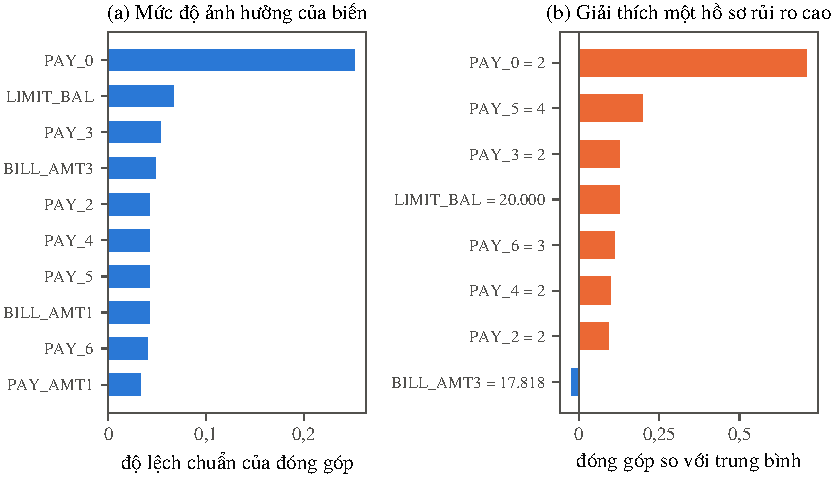
\includegraphics[width=\linewidth]{fig_credit_explain.pdf}
\caption[Mức độ ảnh hưởng của các biến và giải thích một hồ sơ]{(a) Mức độ ảnh hưởng của mười biến quan trọng nhất, đo bằng độ lệch chuẩn của đóng góp $h_i$ trên tập huấn luyện; với các biến định danh, đó là độ lệch chuẩn của tổng đóng góp của các biến chỉ báo tương ứng. (b) Tám đóng góp lớn nhất, so với khách hàng trung bình, của hồ sơ có điểm rủi ro cao nhất trong số các khách hàng vỡ nợ ở tập kiểm tra.}
\label{fig:credit-explain}
\end{figure}

\Cref{fig:credit-explain}a xếp hạng các biến theo mức độ ảnh hưởng. PAY\_0 vượt xa mọi biến khác; tiếp theo, với mức ảnh hưởng nhỏ hơn nhiều, là hạn mức tín dụng, các trạng thái trả nợ của những tháng trước và các số tiền sao kê; các biến nhân khẩu học (học vấn, hôn nhân, giới tính, tuổi) có ảnh hưởng không đáng kể. Vì hàm quyết định~\eqref{eq:additive-decomp} là một tổng, mỗi quyết định của mô hình được giải thích một cách chính xác chứ không phải xấp xỉ: điểm của một khách hàng bằng điểm trung bình trên tập huấn luyện cộng với tổng các đóng góp của từng biến so với khách hàng trung bình. \Cref{fig:credit-explain}b minh họa điều đó với khách hàng có điểm rủi ro cao nhất trong số những người vỡ nợ ở tập kiểm tra. Điểm của khách hàng này là $0{,}96$, trong khi điểm trung bình là $-0{,}56$ và ngưỡng phân loại là $-0{,}44$. Trong phần chênh lệch $1{,}51$ so với điểm trung bình, riêng việc chậm trả hai tháng ở tháng 9 đóng góp $0{,}71$, lịch sử chậm trả ở năm tháng trước đó đóng góp thêm $0{,}63$, và hạn mức thấp ($20.000$ Đài tệ) đóng góp $0{,}13$. Một lời giải thích như vậy có thể được trình bày trực tiếp cho cán bộ tín dụng hay cho khách hàng. Với SVM hạt nhân Gauss hay tổ hợp cây, việc giải thích một quyết định đòi hỏi những kỹ thuật bổ sung, chẳng hạn giá trị SHAP~\cite{lundberg2017}, được tính sau khi huấn luyện và phức tạp hơn nhiều so với việc đọc trực tiếp các hàm $h_i$.

\subsection{Ràng buộc đơn điệu}\label{sec:monotone}

Người làm tín dụng kỳ vọng rằng rủi ro không giảm khi số tháng chậm trả tăng, và không tăng khi hạn mức tín dụng tăng. Mô hình không ràng buộc chỉ thỏa mãn một phần kỳ vọng này: ở cả năm lần chia, ít nhất một trong sáu hàm $h_i$ của các biến PAY có một đoạn với hệ số góc âm ở vùng từ trạng thái $0$ trở đi, và hàm của LIMIT\_BAL có đoạn đi lên ở cả năm lần chia. Như đã phân tích ở trên, đó là những đoạn được ước lượng từ rất ít dữ liệu, không phải là quy luật thật. Một mô hình trái với tri thức nghiệp vụ khó được chấp nhận khi thẩm định, dù độ chính xác của nó cao; vì vậy ta đưa kỳ vọng đơn điệu vào chính bài toán huấn luyện.

Với PWL-SVM cộng tính, điều này có thể làm mà vẫn giữ tính lồi. Gọi $t_{i1}<\dots<t_{iK}$ là các nút của biến thứ $i$ và $s_{i0},\dots,s_{iK}$ là hệ số góc của $h_i$ trên $K+1$ đoạn mà các nút chia ra. Khi đó
\begin{equation}\label{eq:slope-param}
h_i(t)=\sum_{j=0}^{K}s_{ij}\,G_{ij}(t),\qquad
G_{ij}(t)=\min\bigl\{(t-t_{ij})_+,\ t_{i,j+1}-t_{ij}\bigr\},
\end{equation}
với quy ước $t_{i0}=-\infty$, $t_{i,K+1}=+\infty$ (tức $G_{i0}(t)=\min\{t,t_{i1}\}$ và $G_{iK}(t)=(t-t_{iK})_+$): $G_{ij}(t)$ là độ dài phần đoạn thứ $j$ nằm bên trái $t$. Theo \cref{prop:1d}, hệ số của $x(i)$ trong ánh xạ~\eqref{eq:feature-map} bằng $s_{i0}$ và hệ số của $\bigl(x(i)-t_{ij}\bigr)_+$ bằng $s_{ij}-s_{i,j-1}$. Vì vậy~\eqref{eq:slope-param} chỉ là một cách tham số hóa khác của cùng một mô hình, và bài toán~\eqref{eq:ridge} trở thành
\[
\min_{s,\,w_0}\ \frac12\sum_{i=1}^{n}\Bigl[s_{i0}^2+\sum_{j=1}^{K}\bigl(s_{ij}-s_{i,j-1}\bigr)^2\Bigr]+\frac\gamma2\sum_{k=1}^{N}\Bigl(y_k-w_0-\sum_{i=1}^{n}h_i\bigl(x_k(i)\bigr)\Bigr)^2 .
\]
Hàm $h_i$ không giảm khi và chỉ khi $s_{ij}\ge0$ với mọi $j$, và không tăng khi và chỉ khi $s_{ij}\le0$ với mọi $j$; muốn $h_i$ đơn điệu chỉ trên một phần của trục, chẳng hạn trên nửa đường thẳng $t\ge t_{ij_0}$, ta chỉ cần áp các bất đẳng thức đó cho những đoạn nằm trong phần ấy. Thêm các ràng buộc này, ta được một bài toán bình phương tối thiểu với ràng buộc cận trên các biến --- một bài toán lồi, giải được chính xác bằng thuật toán BVLS~\cite{stark1995} có sẵn trong SciPy~\cite{virtanen2020}. Cũng như ở \cref{rem:convex}, tri thức tiên nghiệm được đưa vào mô hình mà không phải từ bỏ tính lồi. Khi không có ràng buộc nào, lời giải trùng với lời giải của \cref{prop:ridge} (sai khác dưới $10^{-9}$), điều được dùng để kiểm tra cài đặt.

\begin{figure}[t]
\centering
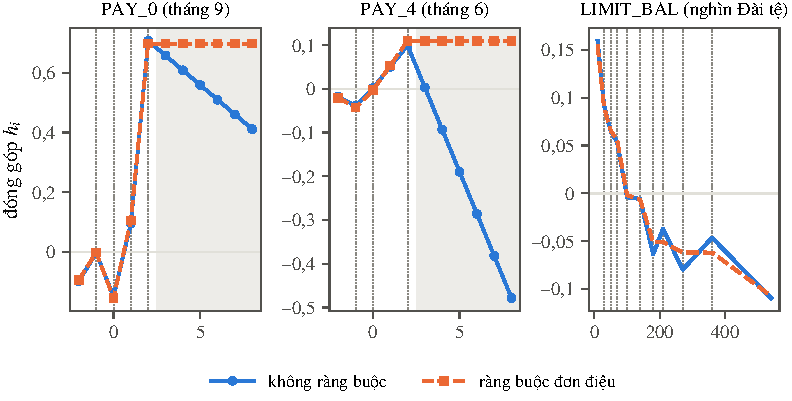
\includegraphics[width=\linewidth]{fig_credit_monotone.pdf}
\caption[Hàm đóng góp khi có và không có ràng buộc đơn điệu]{Hàm đóng góp của PAY\_0, PAY\_4 và LIMIT\_BAL trong mô hình không ràng buộc (nét liền) và mô hình có ràng buộc đơn điệu (nét đứt), lần chia đầu tiên. Vùng tô xám: các trạng thái chậm trả từ ba tháng trở lên, chỉ chiếm chưa tới 2\% số khách hàng.}
\label{fig:credit-monotone}
\end{figure}

Ta ràng buộc sáu hàm của các biến PAY không giảm từ trạng thái $0$ trở đi --- ba mã $-2$, $-1$ và $0$ chỉ những tình trạng không chậm trả khác nhau, không có thứ tự tự nhiên, nên được để tự do --- và hàm của LIMIT\_BAL không tăng trên toàn miền; các biến khác, các nút và hằng số $\gamma$ đã chọn cho mô hình không ràng buộc được giữ nguyên. \Cref{fig:credit-monotone} cho thấy tác động của ràng buộc: sau mức chậm hai tháng, đóng góp của PAY\_0 và PAY\_4 giữ nguyên thay vì giảm, và đường của LIMIT\_BAL trở thành đơn điệu giảm, trong khi hình dạng ở vùng có nhiều dữ liệu hầu như không đổi. Độ chính xác hầu như không thay đổi: AUC trung bình là 0{,}775, so với 0{,}776 của mô hình không ràng buộc, và mô hình có ràng buộc vẫn cao hơn thẻ điểm (0{,}773) (\cref{tab:credit}). Như vậy, với ràng buộc đơn điệu, PWL-LS-SVM cộng tính cho một mô hình vừa chính xác vừa nhất quán với tri thức nghiệp vụ.

\subsection{Khả năng triển khai}

Mô hình PWL-LS-SVM cộng tính trên dữ liệu tín dụng gồm 349 số thực: các nút và hệ số của $20$ đường gấp khúc cho các biến số, hệ số của $6$ biến chỉ báo, hệ số chặn và hai vectơ chuẩn hóa. Để chấm điểm một hồ sơ, với mỗi biến ta chỉ cần xác định giá trị rơi vào đoạn nào giữa các nút rồi tính một hàm bậc nhất, tổng cộng vài trăm phép so sánh, nhân và cộng. Một mô hình như vậy có thể được cài đặt bằng vài dòng lệnh SQL trong kho dữ liệu của ngân hàng, bằng một bảng tính, hoặc trên thiết bị có tài nguyên rất hạn chế, mà không cần thư viện học máy nào; ràng buộc đơn điệu không làm thay đổi cấu trúc này. Việc huấn luyện lại khi có dữ liệu mới chỉ mất chưa tới một giây (\cref{tab:cost-measured}). Để so sánh, SVM hạt nhân Gauss cần lưu khoảng 243.134 số thực, và tổ hợp cây tăng cường gồm từ 34 đến 47 cây quyết định với khoảng 4.636 tham số; cả hai đều khó kiểm tra và giải thích hơn nhiều.

% Generated by code/fill_numbers.py from chuong3_end.tpl -- edit the template, not this file.
% ----------------------------------------------------------------------------
\section{Thảo luận}\label{sec:discussion}

\paragraph{Trả lời các câu hỏi nghiên cứu.} Các thực nghiệm của chương cho phép trả lời bốn câu hỏi nêu ở Mở đầu.

\emph{(CH1) Độ chính xác.} Trên dữ liệu hai chiều, PWL-SVM dạng HH đạt độ chính xác gần SVM hạt nhân Gauss, trừ trên bàn cờ (\cref{tab:exp2d}). Trên mười bộ dữ liệu chuẩn, PWL-C-SVM cộng tính đứng giữa SVM tuyến tính và SVM hạt nhân Gauss: nó kém SVM hạt nhân Gauss trung bình 1{,}4 điểm phần trăm, một khác biệt có ý nghĩa thống kê, và hơn SVM tuyến tính trung bình 1{,}7 điểm, với phần cải thiện tập trung ở những bộ dữ liệu phi tuyến rõ rệt (\cref{tab:bench,tab:wilcoxon}). Nhận định của bài báo gốc rằng PWL-SVM chính xác tương đương SVM hạt nhân Gauss vì vậy không được xác nhận khi thực nghiệm được lặp lại. Trên dữ liệu tín dụng, ngược lại, PWL-LS-SVM cộng tính thuộc nhóm mô hình tốt nhất, cùng với tổ hợp cây tăng cường và thẻ điểm logistic (\cref{tab:credit}).

\emph{(CH2) Chi phí.} Lợi thế về chi phí được xác nhận rõ ràng. Với ánh xạ cộng tính, mô hình nhỏ hơn SVM hạt nhân Gauss từ $2{,}5$ đến $36$ lần trên mười bộ dữ liệu chuẩn và khoảng 690 lần trên dữ liệu tín dụng; thời gian dự đoán nhanh hơn khoảng 200 lần trên Magic và 430 lần trên dữ liệu tín dụng (\cref{tab:cost-measured}). PWL-LS-SVM còn là mô hình phi tuyến huấn luyện nhanh nhất.

\emph{(CH3) Cấu hình.} Ánh xạ cộng tính là lựa chọn mặc định tốt cho dữ liệu dạng bảng: rẻ, dễ diễn giải và thường chính xác nhất trong các dạng ánh xạ. Ánh xạ HH chỉ có lợi khi tương tác giữa các biến đáng kể (bàn cờ, xoắn ốc, Ionosphere); kích thước của nó tăng gần như bậc hai theo số chiều, và quy tắc sinh tham số của bài báo gốc có thể thất bại trên dữ liệu thưa. Độ chính xác bão hòa quanh $M/n=5$--$10$. Hai điều chỉnh nhỏ của đề án --- nút theo phân vị và chuẩn hóa $\|p\|_2=1$ --- cải thiện kết quả và độ ổn định số mà không thay đổi bản chất của phương pháp.

\emph{(CH4) Ứng dụng.} Trên bài toán vỡ nợ thẻ tín dụng, PWL-LS-SVM cộng tính với nút phân vị đạt AUC 0{,}776, chỉ kém một chút so với tổ hợp cây tăng cường (0{,}779) và cao hơn thẻ điểm logistic truyền thống (0{,}773) ở bốn trong năm lần chia, trong khi mô hình chỉ gồm 349 số thực, dự đoán mỗi hồ sơ trong khoảng 0{,}56 micro giây và đọc được như một thẻ điểm tuyến tính từng phần (\cref{fig:credit-shapes}). Khi thêm ràng buộc đơn điệu để mô hình nhất quán với tri thức nghiệp vụ, AUC hầu như không đổi (0{,}775 so với 0{,}776) (Mục~\ref{sec:monotone}).

\paragraph{Khi nào nên dùng PWL-SVM.} Từ các kết quả trên, PWL-SVM cộng tính phù hợp với dữ liệu dạng bảng có số chiều vừa phải, khi mô hình cần nhỏ, dự đoán nhanh hoặc phải giải thích được: chấm điểm tín dụng, các hệ thống nhúng, hay bất cứ bối cảnh nào mà hồi quy logistic đang được dùng vì tính minh bạch. Khi độ chính xác là tiêu chí duy nhất và tài nguyên không bị hạn chế, SVM hạt nhân Gauss, mạng nơ-ron hay tổ hợp cây thường là lựa chọn tốt hơn. Với dữ liệu nhiều chiều, thưa hoặc có tương tác phức tạp, PWL-SVM với các siêu phẳng sinh ngẫu nhiên không phải là công cụ thích hợp; khi đó nên học cả các siêu phẳng, tức là chuyển sang mạng nơ-ron ReLU.

\paragraph{Giới hạn của thực nghiệm.} Kết luận của chương dựa trên mười bộ dữ liệu chuẩn và một bài toán ứng dụng, nên lực của các kiểm định thống kê còn hạn chế. Các lưới tham số được chọn theo khuyến nghị thông dụng và có thể chưa tối ưu cho mọi mô hình; SVM hạt nhân Gauss và mạng nơ-ron trên dữ liệu tín dụng được tinh chỉnh trên mẫu con; thẻ điểm đối chứng dùng một cách rời rạc hóa đơn giản (mười khoảng theo thập phân vị), trong khi các thẻ điểm thực tế thường được xây dựng với các khoảng chọn cẩn thận hơn. Bộ giải LIBLINEAR chính quy hóa nhẹ hệ số chặn, khác với bài toán~\eqref{eq:pwl-c-svm}. Dữ liệu tín dụng được thu thập ở Đài Loan năm 2005, nên các hàm đóng góp tìm được minh họa phương pháp chứ không nhất thiết phản ánh hành vi của khách hàng Việt Nam hiện nay. Cuối cùng, thời gian đo được phụ thuộc vào phần cứng và cách cài đặt.

% ----------------------------------------------------------------------------
\section*{Tiểu kết Chương 3}
\phantomsection\addcontentsline{toc}{section}{Tiểu kết Chương 3}

Chương 3 đã cài đặt PWL-SVM, kiểm chứng tính đúng đắn của cài đặt bằng các phép thử số, và đánh giá phương pháp qua ba lớp thực nghiệm: dữ liệu hai chiều, mười bộ dữ liệu chuẩn và một bài toán ứng dụng. Kết quả cho một bức tranh nhất quán: PWL-SVM không chính xác hơn các mô hình phi tuyến mạnh như SVM hạt nhân Gauss, nhưng nó cho những mô hình nhỏ hơn từ vài lần đến hàng trăm lần, dự đoán nhanh hơn nhiều, huấn luyện bằng một bài toán lồi và, với ánh xạ cộng tính, có thể đọc được từng thành phần. Trên bài toán dự báo vỡ nợ thẻ tín dụng, nơi các tính chất đó được coi trọng, PWL-LS-SVM cộng tính với nút phân vị đạt độ chính xác ngang những mô hình tốt nhất, và với ràng buộc đơn điệu, cho một mô hình nhất quán với tri thức nghiệp vụ mà không mất độ chính xác.


% Generated by code/fill_numbers.py from ketluan.tpl -- edit the template, not this file.
% ============================================================================
%  KẾT LUẬN
% ============================================================================
\unchapter{KẾT LUẬN VÀ HƯỚNG PHÁT TRIỂN}

\section*{Kết quả đạt được}

Đề án đã nghiên cứu một cách có hệ thống phương pháp SVM với ánh xạ đặc trưng tuyến tính từng phần của Huang, Mehrkanoon và Suykens~\cite{huang2013}, cài đặt lại phương pháp, đánh giá nó bằng thực nghiệm lặp lại và áp dụng vào bài toán dự báo vỡ nợ thẻ tín dụng. Các kết quả chính như sau.

\emph{Về lý thuyết.} Đề án đã trình bày đầy đủ chuỗi lập luận từ tập lồi, định lý siêu phẳng phân tách và đối ngẫu Lagrange đến SVM lề cứng, lề mềm và LS-SVM, rồi từ các định lý biểu diễn hàm tuyến tính từng phần đến ánh xạ đặc trưng tuyến tính từng phần. Bên cạnh việc viết lại các chứng minh, đề án đã đưa ra một chứng minh ngắn hơn cho định lý biểu diễn tập tuyến tính từng phần, chỉ ra rằng hàm xây dựng trong chứng minh luôn không âm nên chỉ mô tả biên chứ không phải một bộ phân loại, chứng minh rằng phần tuyến tính của SVM hạt nhân giao triệt tiêu nhờ ràng buộc của bài toán đối ngẫu, chứng minh rằng hiệu hai hàm khoảng cách của phương pháp láng giềng gần nhất là hàm tuyến tính từng phần, chỉ ra dạng gốc của PWL-LS-SVM chính là hồi quy ridge, nêu một giới hạn cơ bản của mô hình cộng tính đối với cấu trúc kiểu XOR, và chỉ ra rằng tham số hóa theo hệ số góc cho phép đưa ràng buộc đơn điệu vào PWL-SVM cộng tính mà bài toán vẫn là lồi.

\emph{Về cài đặt.} Đề án cung cấp một cài đặt bằng Python, tương thích với scikit-learn, cho ba dạng ánh xạ và hai mô hình PWL-C-SVM và PWL-LS-SVM, cùng hai tùy chọn mới là đặt nút theo phân vị và chuẩn hóa siêu phẳng, và một biến thể PWL-LS-SVM cộng tính có ràng buộc đơn điệu. Tính đúng đắn của cài đặt được kiểm chứng bằng số: nghiệm gốc và nghiệm đối ngẫu trùng nhau đến sai số làm tròn.

\emph{Về thực nghiệm.} Trên mười bộ dữ liệu chuẩn, PWL-SVM cộng tính chính xác hơn SVM tuyến tính nhưng kém SVM hạt nhân Gauss trung bình 1{,}4 điểm phần trăm; nhận định về độ chính xác của bài báo gốc, vốn dựa trên một lần chia dữ liệu, chỉ được xác nhận một phần. Ngược lại, lợi thế về kích thước mô hình và tốc độ dự đoán được xác nhận rõ ràng: mô hình nhỏ hơn SVM hạt nhân Gauss từ $2{,}5$ đến $36$ lần trên các bộ dữ liệu chuẩn, và dự đoán nhanh hơn khoảng 200 lần trên Magic. Các thực nghiệm cũng cho thấy ánh xạ cộng tính là lựa chọn mặc định hợp lý, số đặc trưng $M=5n$ đến $10n$ là đủ, còn quy tắc sinh siêu phẳng của bài báo gốc có thể gây sự cố số trên dữ liệu thưa và nên được thay bằng quy tắc chuẩn hóa $\|p\|_2=1$.

\emph{Về ứng dụng.} Trên dữ liệu vỡ nợ của $30.000$ chủ thẻ tín dụng, PWL-LS-SVM cộng tính với nút phân vị đạt AUC 0{,}776, chỉ kém một chút so với tổ hợp cây tăng cường (0{,}779), cao hơn thẻ điểm logistic trên các biến rời rạc hóa (0{,}773) và cao hơn rõ rệt hồi quy logistic trên biến gốc (0{,}724) cũng như SVM hạt nhân Gauss (0{,}716). Mô hình chỉ gồm 349 số thực, dự đoán mỗi hồ sơ trong khoảng 0{,}56 micro giây, và mỗi biến có một hàm đóng góp tuyến tính từng phần đọc được, phù hợp với yêu cầu minh bạch của chấm điểm tín dụng. Khi thêm ràng buộc đơn điệu cho các biến trạng thái trả nợ và hạn mức, mô hình trở nên nhất quán với tri thức nghiệp vụ, trong khi AUC hầu như không đổi (0{,}775 so với 0{,}776).

\section*{Hạn chế}

Các tham số phi tuyến của ánh xạ được chọn theo quy tắc cố định hoặc ngẫu nhiên chứ không được học từ dữ liệu, nên PWL-SVM dạng HH kém hiệu quả trên dữ liệu nhiều chiều. Các định lý biểu diễn chỉ khẳng định sự tồn tại và không cho biết cần bao nhiêu đặc trưng. Thực nghiệm dựa trên mười bộ dữ liệu chuẩn và một bài toán ứng dụng, với các lưới tham số và một thẻ điểm đối chứng được xây dựng theo cách đơn giản; dữ liệu tín dụng được thu thập ở Đài Loan năm 2005 và có thể không đại diện cho khách hàng Việt Nam hiện nay. Đề án chỉ xét bài toán phân loại nhị phân, và dạng siêu phẳng bản lề tổng quát chỉ được thử trên dữ liệu hai chiều.

\section*{Hướng phát triển}

Từ các kết quả và hạn chế trên, có bốn hướng phát triển tự nhiên. Thứ nhất, dùng chính quy hóa $\ell_1$ như trong Mục~5 của~\cite{huang2013} để tự động loại bớt các đặc trưng thừa và thu được những biên gồm ít mảnh hơn. Thứ hai, mở rộng cách tiếp cận ở Mục~\ref{sec:monotone} cho những dạng tri thức nghiệp vụ khác, chẳng hạn ràng buộc lồi (\cref{rem:convex}) hay ràng buộc về độ trơn của các hàm đóng góp, và chọn hằng số $\gamma$ đồng thời với các ràng buộc. Thứ ba, học cả tham số của các siêu phẳng bản lề, chẳng hạn bằng cách xen kẽ giữa tối ưu các siêu phẳng và giải SVM, tiến tới các mạng nơ-ron tuyến tính từng phần~\cite{tao2022}. Thứ tư, mở rộng phương pháp cho bài toán nhiều lớp và hồi quy, và kiểm nghiệm trên dữ liệu tín dụng của Việt Nam khi có điều kiện tiếp cận.


% ------------------------------------------------------------ phần cuối
\backmatter
% ============================================================================
%  TÀI LIỆU THAM KHẢO — xếp theo quy định: tiếng Việt trước (theo tên),
%  tiếng Anh sau (theo họ tác giả thứ nhất)
% ============================================================================
\renewcommand{\bibname}{TÀI LIỆU THAM KHẢO}
\begingroup
\small
\setstretch{1.2}
\begin{thebibliography}{99}
\addcontentsline{toc}{chapter}{Tài liệu tham khảo}
\setlength{\itemsep}{2pt}

\item[]\hspace*{-\labelwidth}\hspace*{-\labelsep}\textbf{Tiếng Việt}

\bibitem{dovanluu2000} Đỗ Văn Lưu, Phan Huy Khải (2000), \emph{Giải tích lồi}, Nhà xuất bản Khoa học và Kỹ thuật, Hà Nội.

\bibitem{vuhuutiep2018} Vũ Hữu Tiệp (2018), \emph{Machine Learning cơ bản}, Nhà xuất bản Khoa học và Kỹ thuật, Hà Nội.

\item[]\hspace*{-\labelwidth}\hspace*{-\labelsep}\textbf{Tiếng Anh}

\bibitem{arora2018} Arora R., Basu A., Mianjy P., Mukherjee A. (2018), “Understanding deep neural networks with rectified linear units”, in: \emph{International Conference on Learning Representations (ICLR 2018)}.

\bibitem{baesens2003} Baesens B., Van Gestel T., Viaene S., Stepanova M., Suykens J.A.K., Vanthienen J. (2003), “Benchmarking state-of-the-art classification algorithms for credit scoring”, \emph{Journal of the Operational Research Society}, 54(6), pp.~627--635.

\bibitem{bagirov2005} Bagirov A.M. (2005), “Max--min separability”, \emph{Optimization Methods and Software}, 20(2--3), pp.~277--296.

\bibitem{bennett2000} Bennett K.P., Bredensteiner E.J. (2000), “Duality and geometry in SVM classifiers”, in: \emph{Proceedings of the 17th International Conference on Machine Learning (ICML)}, pp.~57--64.

\bibitem{boser1992} Boser B.E., Guyon I.M., Vapnik V.N. (1992), “A training algorithm for optimal margin classifiers”, in: \emph{Proceedings of the 5th Annual Workshop on Computational Learning Theory (COLT)}, ACM, pp.~144--152.

\bibitem{boyd2004} Boyd S., Vandenberghe L. (2004), \emph{Convex Optimization}, Cambridge University Press, Cambridge.

\bibitem{breiman1993} Breiman L. (1993), “Hinging hyperplanes for regression, classification, and function approximation”, \emph{IEEE Transactions on Information Theory}, 39(3), pp.~999--1013.

\bibitem{canu2005} Canu S., Grandvalet Y., Guigue V., Rakotomamonjy A. (2005), \emph{SVM and Kernel Methods Matlab Toolbox}, Perception Systèmes et Information, INSA de Rouen, Rouen.

\bibitem{chang2011} Chang C.-C., Lin C.-J. (2011), “LIBSVM: a library for support vector machines”, \emph{ACM Transactions on Intelligent Systems and Technology}, 2(3), Article~27.

\bibitem{chua1977} Chua L.O., Kang S.M. (1977), “Section-wise piecewise-linear functions: canonical representation, properties, and applications”, \emph{Proceedings of the IEEE}, 65(6), pp.~915--929.

\bibitem{cortes1995} Cortes C., Vapnik V. (1995), “Support-vector networks”, \emph{Machine Learning}, 20(3), pp.~273--297.

\bibitem{cover1967} Cover T., Hart P. (1967), “Nearest neighbor pattern classification”, \emph{IEEE Transactions on Information Theory}, 13(1), pp.~21--27.

\bibitem{demsar2006} Demšar J. (2006), “Statistical comparisons of classifiers over multiple data sets”, \emph{Journal of Machine Learning Research}, 7, pp.~1--30.

\bibitem{do2017} Do T.-N., Poulet F. (2017), “Parallel learning of local SVM algorithms for classifying large datasets”, in: \emph{Transactions on Large-Scale Data- and Knowledge-Centered Systems XXXI}, Lecture Notes in Computer Science 10140, Springer, Berlin, Heidelberg.

\bibitem{fan2008} Fan R.-E., Chang K.-W., Hsieh C.-J., Wang X.-R., Lin C.-J. (2008), “LIBLINEAR: a library for large linear classification”, \emph{Journal of Machine Learning Research}, 9, pp.~1871--1874.

\bibitem{fawcett2006} Fawcett T. (2006), “An introduction to ROC analysis”, \emph{Pattern Recognition Letters}, 27(8), pp.~861--874.

\bibitem{freund1995} Freund Y., Schapire R.E. (1995), “A decision-theoretic generalization of on-line learning and an application to boosting”, in: \emph{Computational Learning Theory (EuroCOLT 1995)}, Lecture Notes in Computer Science 904, Springer, pp.~23--37.

\bibitem{friedman2001} Friedman J.H. (2001), “Greedy function approximation: a gradient boosting machine”, \emph{The Annals of Statistics}, 29(5), pp.~1189--1232.

\bibitem{goodfellow2013} Goodfellow I., Warde-Farley D., Mirza M., Courville A., Bengio Y. (2013), “Maxout networks”, in: \emph{Proceedings of the 30th International Conference on Machine Learning (ICML)}, pp.~1319--1327.

\bibitem{harris2020} Harris C.R. và cộng sự (2020), “Array programming with NumPy”, \emph{Nature}, 585(7825), pp.~357--362.

\bibitem{hastie1990} Hastie T., Tibshirani R. (1990), \emph{Generalized Additive Models}, Chapman \& Hall, London.

\bibitem{hsu2003} Hsu C.-W., Chang C.-C., Lin C.-J. (2003), \emph{A Practical Guide to Support Vector Classification}, Technical report, Department of Computer Science, National Taiwan University.

\bibitem{huanggb2006} Huang G.-B., Zhu Q.-Y., Siew C.-K. (2006), “Extreme learning machine: theory and applications”, \emph{Neurocomputing}, 70(1--3), pp.~489--501.

\bibitem{huang2013} Huang X., Mehrkanoon S., Suykens J.A.K. (2013), “Support vector machines with piecewise linear feature mapping”, \emph{Neurocomputing}, 117, pp.~118--127.

\bibitem{kelly_uci} Kelly M., Longjohn R., Nottingham K., \emph{The UCI Machine Learning Repository}, \texttt{https://archive.ics.uci.edu} (truy cập tháng 9/2026).

\bibitem{kostin2006} Kostin A. (2006), “A simple and fast multi-class piecewise linear pattern classifier”, \emph{Pattern Recognition}, 39(11), pp.~1949--1962.

\bibitem{lessmann2015} Lessmann S., Baesens B., Seow H.-V., Thomas L.C. (2015), “Benchmarking state-of-the-art classification algorithms for credit scoring: an update of research”, \emph{European Journal of Operational Research}, 247(1), pp.~124--136.

\bibitem{li2011} Li Y., Liu B., Yang X., Fu Y., Li H. (2011), “Multiconlitron: a general piecewise linear classifier”, \emph{IEEE Transactions on Neural Networks}, 22(2), pp.~276--289.

\bibitem{liu1989} Liu D.C., Nocedal J. (1989), “On the limited memory BFGS method for large scale optimization”, \emph{Mathematical Programming}, 45(1--3), pp.~503--528.

\bibitem{lundberg2017} Lundberg S.M., Lee S.-I. (2017), “A unified approach to interpreting model predictions”, in: \emph{Advances in Neural Information Processing Systems 30}, pp.~4765--4774.

\bibitem{maji2008} Maji S., Berg A.C., Malik J. (2008), “Classification using intersection kernel support vector machines is efficient”, in: \emph{IEEE Conference on Computer Vision and Pattern Recognition (CVPR)}, pp.~1--8.

\bibitem{mangasarian1968} Mangasarian O.L. (1968), “Multisurface method of pattern separation”, \emph{IEEE Transactions on Information Theory}, 14(6), pp.~801--807.

\bibitem{ovchinnikov2002} Ovchinnikov S. (2002), “Max-min representation of piecewise linear functions”, \emph{Beiträge zur Algebra und Geometrie}, 43(1), pp.~297--302.

\bibitem{pedregosa2011} Pedregosa F. và cộng sự (2011), “Scikit-learn: machine learning in Python”, \emph{Journal of Machine Learning Research}, 12, pp.~2825--2830.

\bibitem{platt1999} Platt J.C. (1999), “Fast training of support vector machines using sequential minimal optimization”, in: \emph{Advances in Kernel Methods: Support Vector Learning}, MIT Press, Cambridge, MA, pp.~185--208.

\bibitem{rahimi2007} Rahimi A., Recht B. (2007), “Random features for large-scale kernel machines”, in: \emph{Advances in Neural Information Processing Systems 20}, pp.~1177--1184.

\bibitem{scholkopf2002} Schölkopf B., Smola A.J. (2002), \emph{Learning with Kernels}, MIT Press, Cambridge, MA.

\bibitem{sklansky1980} Sklansky J., Michelotti L. (1980), “Locally trained piecewise linear classifiers”, \emph{IEEE Transactions on Pattern Analysis and Machine Intelligence}, 2(2), pp.~101--111.

\bibitem{stark1995} Stark P.B., Parker R.L. (1995), “Bounded-variable least-squares: an algorithm and applications”, \emph{Computational Statistics}, 10(2), pp.~129--141.

\bibitem{suykens1999ls} Suykens J.A.K., Vandewalle J. (1999), “Least squares support vector machine classifiers”, \emph{Neural Processing Letters}, 9(3), pp.~293--300.

\bibitem{suykens1999mlp} Suykens J.A.K., Vandewalle J. (1999), “Training multilayer perceptron classifiers based on a modified support vector method”, \emph{IEEE Transactions on Neural Networks}, 10(4), pp.~907--911.

\bibitem{suykens2002} Suykens J.A.K., Van Gestel T., De Brabanter J., De Moor B., Vandewalle J. (2002), \emph{Least Squares Support Vector Machines}, World Scientific, Singapore.

\bibitem{tao2022} Tao Q., Li L., Huang X., Xi X., Wang S., Suykens J.A.K. (2022), “Piecewise linear neural networks and deep learning”, \emph{Nature Reviews Methods Primers}, 2, Article~42.

\bibitem{tarela1999} Tarela J.M., Martínez M.V. (1999), “Region configurations for realizability of lattice piecewise-linear models”, \emph{Mathematical and Computer Modelling}, 30(11--12), pp.~17--27.

\bibitem{tenmoto1998} Tenmoto H., Kudo M., Shimbo M. (1998), “Piecewise linear classifiers with an appropriate number of hyperplanes”, \emph{Pattern Recognition}, 31(11), pp.~1627--1634.

\bibitem{thomas2002} Thomas L.C., Edelman D.B., Crook J.N. (2002), \emph{Credit Scoring and Its Applications}, SIAM, Philadelphia.

\bibitem{vanschoren2013} Vanschoren J., van Rijn J.N., Bischl B., Torgo L. (2013), “OpenML: networked science in machine learning”, \emph{SIGKDD Explorations}, 15(2), pp.~49--60.

\bibitem{vapnik1998} Vapnik V.N. (1998), \emph{Statistical Learning Theory}, Wiley, New York.

\bibitem{virtanen2020} Virtanen P. và cộng sự (2020), “SciPy 1.0: fundamental algorithms for scientific computing in Python”, \emph{Nature Methods}, 17(3), pp.~261--272.

\bibitem{wang2005} Wang S., Sun X. (2005), “Generalization of hinging hyperplanes”, \emph{IEEE Transactions on Information Theory}, 51(12), pp.~4425--4431.

\bibitem{webb2010} Webb D. (2010), \emph{Efficient Piecewise Linear Classifiers and Applications}, PhD thesis, University of Ballarat, Australia.

\bibitem{yeh2009} Yeh I.-C., Lien C.-H. (2009), “The comparisons of data mining techniques for the predictive accuracy of probability of default of credit card clients”, \emph{Expert Systems with Applications}, 36(2), pp.~2473--2480.

\end{thebibliography}
\endgroup

% ============================================================================
%  PHỤ LỤC
% ============================================================================
\unchapter{PHỤ LỤC}
\setcounter{table}{0}\renewcommand{\thetable}{PL.\arabic{table}}

\section*{A. Mã nguồn chính}
\phantomsection\addcontentsline{toc}{section}{A. Mã nguồn chính}

Toàn bộ mã nguồn của đề án gồm mô-đun \texttt{pwlsvm.py} (ánh xạ đặc trưng và mô hình), mô-đun \texttt{baselines.py} (LS-SVM hạt nhân Gauss, SVM hạt nhân giao), các tệp nạp dữ liệu và các tệp thực nghiệm; mỗi hình và bảng của Chương~\ref{chap:3} được sinh bởi một tệp riêng, với hạt giống ngẫu nhiên cố định. Dưới đây là phần cốt lõi của \texttt{pwlsvm.py}, đã lược bớt phần kiểm tra đầu vào và chú thích.

\begin{lstlisting}
import numpy as np
from sklearn.preprocessing import MinMaxScaler
from sklearn.svm import SVC, LinearSVC

def random_hyperplane(rng, lo, hi):
    """p^T x + q = 0 through n uniform points of [lo, hi],
    with p(1) = +1 or -1."""
    n = lo.size
    while True:
        U = rng.uniform(lo, hi, size=(n, n))   # rows u_j
        s = rng.choice([-1.0, 1.0])            # p(1)
        A = np.hstack([U[:, 1:], np.ones((n, 1))])
        if abs(np.linalg.det(A)) > 1e-12:
            sol = np.linalg.solve(A, -s * U[:, 0])
            return np.r_[s, sol[:-1]], sol[-1]

class PWLFeatures:
    """phi(x) = [x(1..n), hinge features]."""
    def __init__(self, kind, m_per_dim, knots="uniform",
                 normalize=False, random_state=None): ...

    def fit(self, X):
        n = X.shape[1]; lo, hi = X.min(0), X.max(0)
        if self.kind == "additive":        # additive map
            S = int(self.m_per_dim); f = np.arange(1, S) / S
            axes, knots = [], []
            for i in range(n):
                if self.knots == "uniform":
                    q = lo[i] + (hi[i] - lo[i]) * f
                else:                       # quantile knots
                    q = np.unique(np.quantile(X[:, i], f))
                    q = q[(q > lo[i]) & (q < hi[i])]
                axes.append(np.full(q.size, i)); knots.append(q)
            self.axis_ = np.concatenate(axes)
            self.knot_ = np.concatenate(knots)
        else:                               # HH or GHH map
            rng = np.random.default_rng(self.random_state)
            D = int(round((self.m_per_dim - 1) * n))
            k = 1 if self.kind == "hh" else n
            P, q = np.empty((D, k, n)), np.empty((D, k))
            for m in range(D):
                for j in range(k):
                    P[m, j], q[m, j] = random_hyperplane(rng, lo, hi)
            if self.normalize:              # ||p||_2 = 1
                s = np.linalg.norm(P, axis=2)
                P, q = P / s[..., None], q / s
            self.P_, self.q_ = P, q
        return self

    def transform(self, X):
        if self.kind == "additive":
            H = np.maximum(0.0, X[:, self.axis_] - self.knot_)
        else:
            D, k, n = self.P_.shape
            Z = X @ self.P_.reshape(D * k, n).T + self.q_.ravel()
            H = np.maximum(0.0, Z.reshape(len(X), D, k).max(2))
        return np.hstack([X, H])

class PWLSVM:
    """PWL-C-SVM (loss="hinge") or PWL-LS-SVM ("squared")."""
    def fit(self, X, y):
        self.scaler_ = MinMaxScaler().fit(X)
        Xs = self.scaler_.transform(X)
        self.features_ = PWLFeatures(self.kind, self.m_per_dim,
            self.knots, self.normalize, self.random_state).fit(Xs)
        Phi = self.features_.transform(Xs)
        if self.loss == "squared":           # ridge primal
            t = np.where(y == y.max(), 1.0, -1.0)
            mu, tb = Phi.mean(0), t.mean()
            Pc = Phi - mu
            A = Pc.T @ Pc + np.eye(Phi.shape[1]) / self.C
            self.coef_ = np.linalg.solve(A, Pc.T @ (t - tb))
            self.intercept_ = tb - mu @ self.coef_
        elif self.solver == "libsvm":        # exact dual
            m = SVC(kernel="linear", C=self.C).fit(Phi, y)
            self.coef_, self.intercept_ = m.coef_[0], m.intercept_[0]
        else:                                # LIBLINEAR
            m = LinearSVC(loss="hinge", C=self.C, dual=True,
                          intercept_scaling=10.0).fit(Phi, y)
            self.coef_, self.intercept_ = m.coef_[0], m.intercept_[0]
        return self

    def decision_function(self, X):
        Phi = self.features_.transform(self.scaler_.transform(X))
        return Phi @ self.coef_ + self.intercept_
\end{lstlisting}

\noindent Ví dụ sử dụng, với cú pháp quen thuộc của scikit-learn:

\begin{lstlisting}
model = PWLSVM(kind="additive", m_per_dim=10, loss="squared",
               knots="quantile", C=2.0).fit(X_train, y_train)
scores = model.decision_function(X_test)
\end{lstlisting}

\noindent Phần cốt lõi của \texttt{pwlsvm\_monotone.py} (Mục~\ref{sec:monotone}): mỗi biến được tham số hóa bởi các hệ số góc $s_{ij}$ theo~\eqref{eq:slope-param}, và ràng buộc đơn điệu trở thành ràng buộc cận trên các $s_{ij}$.

\begin{lstlisting}
from scipy.linalg import block_diag
from scipy.optimize import lsq_linear

def fit_monotone(Xs, t, knots, C, sign):
    """Xs: inputs in [0, 1]; t: labels +-1; knots[i]: sorted
    knots of input i; sign[i]: +1, -1 or 0 for each segment."""
    G, D, lb, ub = [], [], [], []
    for i, tk in enumerate(knots):
        x, K = Xs[:, i], len(tk)
        g = np.empty((len(x), K + 1))      # the G_ij
        g[:, 0] = np.minimum(x, tk[0]) if K else x
        for j in range(1, K):
            g[:, j] = np.clip(x - tk[j-1], 0, tk[j] - tk[j-1])
        if K:
            g[:, K] = np.maximum(0, x - tk[K-1])
        G.append(g)
        D.append(np.eye(K + 1) - np.eye(K + 1, k=-1))   # s -> (a, c)
        lb.append(np.where(sign[i] > 0, 0.0, -np.inf))
        ub.append(np.where(sign[i] < 0, 0.0, np.inf))
    G, D = np.hstack(G), block_diag(*D)
    gbar, tbar = G.mean(0), t.mean()           # unpenalized bias
    A = np.vstack([np.sqrt(C) * (G - gbar), D])
    b = np.r_[np.sqrt(C) * (t - tbar), np.zeros(len(D))]
    s = lsq_linear(A, b, bounds=(np.concatenate(lb),
                   np.concatenate(ub)), method="bvls").x
    return s, tbar - gbar @ s                  # slopes, bias
\end{lstlisting}

\section*{B. Kết quả đầy đủ trên mười bộ dữ liệu chuẩn}
\phantomsection\addcontentsline{toc}{section}{B. Kết quả đầy đủ trên mười bộ dữ liệu chuẩn}

\Cref{tab:appendix-bench} bổ sung cho \cref{tab:bench} độ lệch chuẩn của độ chính xác qua mười lần chia (năm lần với Spambase) và kích thước của từng mô hình. Kích thước được tính là số thực cần lưu để dự đoán, gồm cả hai vectơ giá trị nhỏ nhất và lớn nhất dùng để chuẩn hóa: với SVM hạt nhân và kNN là các điểm được lưu cùng hệ số của chúng; với MLP là mọi trọng số và độ lệch; với PWL-SVM là các nút hoặc tham số của siêu phẳng cùng vectơ $w$ và $w_0$.

\begin{table}[p]
\centering
\caption[Độ chính xác đầy đủ trên mười bộ dữ liệu chuẩn]{Độ chính xác trên tập kiểm tra (\%, trung bình $\pm$ độ lệch chuẩn qua $10$ lần chia, $5$ lần với Spambase) và kích thước mô hình (số thực cần lưu, trung vị).}
\label{tab:appendix-bench}
\footnotesize
\setlength{\tabcolsep}{3pt}
\renewcommand{\arraystretch}{1.15}
\begin{tabular}{@{}l c c c c c@{}}
\toprule
\textbf{Dữ liệu} & \begin{tabular}[b]{@{}c@{}}SVM\\tuyến tính\end{tabular} & \begin{tabular}[b]{@{}c@{}}SVM-\\RBF\end{tabular} & \begin{tabular}[b]{@{}c@{}}LS-SVM-\\RBF\end{tabular} & \begin{tabular}[b]{@{}c@{}}kNN\\$(k=1)$\end{tabular} & \begin{tabular}[b]{@{}c@{}}Ik-\\SVM\end{tabular}\\
\midrule
Haberman & $72{,}5\pm1{,}1$ & $73{,}3\pm1{,}9$ & $73{,}4\pm1{,}8$ & $65{,}7\pm1{,}5$ & $72{,}0\pm1{,}4$\\
Transfusion & $76{,}5\pm0{,}4$ & $77{,}6\pm1{,}4$ & $77{,}7\pm1{,}5$ & $68{,}4\pm2{,}0$ & $76{,}7\pm0{,}9$\\
Banknote & $98{,}6\pm0{,}4$ & $100{,}0\pm0{,}0$ & $100{,}0\pm0{,}1$ & $99{,}8\pm0{,}1$ & $99{,}9\pm0{,}2$\\
Pima & $76{,}7\pm1{,}6$ & $76{,}1\pm2{,}3$ & $76{,}6\pm2{,}0$ & $70{,}8\pm2{,}1$ & $76{,}0\pm1{,}7$\\
Breast & $96{,}6\pm0{,}5$ & $96{,}5\pm0{,}9$ & $96{,}4\pm0{,}9$ & $95{,}3\pm1{,}0$ & $96{,}4\pm0{,}7$\\
Magic & $79{,}0\pm0{,}2$ & $85{,}5\pm0{,}4$ & $85{,}6\pm0{,}4$ & $78{,}3\pm0{,}5$ & $85{,}0\pm0{,}4$\\
Parkinsons & $85{,}4\pm2{,}3$ & $89{,}9\pm3{,}5$ & $91{,}4\pm3{,}8$ & $93{,}7\pm2{,}3$ & $89{,}4\pm3{,}1$\\
Ionosphere & $86{,}2\pm1{,}5$ & $93{,}4\pm1{,}6$ & $93{,}8\pm1{,}8$ & $86{,}4\pm3{,}3$ & $91{,}1\pm1{,}8$\\
Spambase & $93{,}0\pm0{,}6$ & $93{,}6\pm0{,}4$ & $93{,}4\pm0{,}5$ & $88{,}8\pm0{,}8$ & $94{,}6\pm0{,}3$\\
Sonar & $75{,}2\pm4{,}6$ & $84{,}3\pm2{,}9$ & $84{,}5\pm4{,}3$ & $81{,}2\pm2{,}9$ & $82{,}0\pm4{,}7$\\
\midrule
\quad số thực, Haberman & 10 & 325 & 619 & 618 & 367\\
\quad số thực, Transfusion & 13 & 959 & 1.879 & 1.878 & 984\\
\quad số thực, Banknote & 13 & 282 & 3.439 & 3.438 & 329\\
\quad số thực, Pima & 25 & 2.042 & 3.473 & 3.472 & 2.200\\
\quad số thực, Breast & 28 & 469 & 3.509 & 3.508 & 464\\
\quad số thực, Magic & 31 & 7.694 & 22.021 & 22.020 & 9.008\\
\quad số thực, Parkinsons & 67 & 1.276 & 2.276 & 2.275 & 1.057\\
\quad số thực, Ionosphere & 100 & 2.855 & 6.017 & 6.016 & 2.668\\
\quad số thực, Spambase & 172 & 29.753 & 133.515 & 133.514 & 29.869\\
\quad số thực, Sonar & 181 & 5.458 & 6.465 & 6.464 & 4.696\\
\bottomrule
\end{tabular}
\par\medskip
\begin{tabular}{@{}l c c c c@{}}
\toprule
\textbf{Dữ liệu} & \begin{tabular}[b]{@{}c@{}}MLP-\\ReLU\end{tabular} & \begin{tabular}[b]{@{}c@{}}PWL-C\\cộng tính\end{tabular} & \begin{tabular}[b]{@{}c@{}}PWL-LS\\cộng tính\end{tabular} & \begin{tabular}[b]{@{}c@{}}PWL-C\\HH\end{tabular}\\
\midrule
Haberman & $72{,}4\pm1{,}6$ & $73{,}2\pm1{,}9$ & $72{,}6\pm2{,}1$ & $73{,}5\pm1{,}5$\\
Transfusion & $78{,}6\pm1{,}5$ & $76{,}3\pm0{,}5$ & $77{,}4\pm0{,}8$ & $76{,}3\pm2{,}7$\\
Banknote & $99{,}9\pm0{,}1$ & $99{,}9\pm0{,}1$ & $99{,}5\pm0{,}3$ & $99{,}9\pm0{,}1$\\
Pima & $76{,}7\pm1{,}7$ & $76{,}3\pm1{,}2$ & $76{,}5\pm1{,}5$ & $76{,}2\pm1{,}7$\\
Breast & $96{,}8\pm0{,}8$ & $96{,}3\pm0{,}9$ & $96{,}0\pm0{,}7$ & $95{,}6\pm1{,}3$\\
Magic & $85{,}7\pm0{,}2$ & $84{,}8\pm0{,}3$ & $84{,}4\pm0{,}3$ & $84{,}3\pm1{,}4$\\
Parkinsons & $90{,}6\pm3{,}7$ & $86{,}2\pm2{,}3$ & $89{,}3\pm3{,}0$ & $85{,}5\pm2{,}7$\\
Ionosphere & $88{,}0\pm2{,}7$ & $89{,}7\pm2{,}0$ & $87{,}7\pm3{,}7$ & $87{,}0\pm3{,}3$\\
Spambase & $93{,}9\pm0{,}2$ & $93{,}4\pm0{,}4$ & $92{,}6\pm0{,}4$ & $82{,}1\pm23{,}5$\\
Sonar & $81{,}9\pm4{,}4$ & $80{,}2\pm4{,}1$ & $79{,}8\pm4{,}3$ & $76{,}2\pm2{,}4$\\
\midrule
\quad số thực, Haberman & 142 & 64 & 64 & 145\\
\quad số thực, Transfusion & 225 & 85 & 85 & 229\\
\quad số thực, Banknote & 225 & 85 & 85 & 229\\
\quad số thực, Pima & 737 & 169 & 169 & 745\\
\quad số thực, Breast & 910 & 190 & 190 & 919\\
\quad số thực, Magic & 1.101 & 211 & 211 & 1.111\\
\quad số thực, Parkinsons & 4.797 & 463 & 463 & 4.819\\
\quad số thực, Ionosphere & 10.462 & 694 & 694 & 10.495\\
\quad số thực, Spambase & 30.382 & 1.198 & 1.198 & 30.439\\
\quad số thực, Sonar & 33.601 & 1.261 & 1.261 & 33.661\\
\bottomrule
\end{tabular}
\par\medskip
\end{table}


\section*{C. Nguồn dữ liệu}
\phantomsection\addcontentsline{toc}{section}{C. Nguồn dữ liệu}

Mọi bộ dữ liệu đều là bản sao trên kho OpenML~\cite{vanschoren2013} của các bộ dữ liệu trong kho UCI~\cite{kelly_uci}, được tải bằng hàm \texttt{fetch\_openml} của scikit-learn theo mã số ở \cref{tab:sources}. Với Breast, $16$ giá trị thiếu của biến \emph{Bare Nuclei} được thay bằng trung vị; với Ionosphere, cột thứ hai (hằng số) được loại bỏ.

\begin{table}[h]
\centering
\caption[Mã số OpenML của các bộ dữ liệu]{Mã số OpenML và nhãn được coi là lớp $+1$.}
\label{tab:sources}
\small
\renewcommand{\arraystretch}{1.15}
\begin{tabular}{@{}l r l@{\qquad}l r l@{}}
\toprule
\textbf{Dữ liệu} & \textbf{Mã số} & \textbf{Lớp $+1$} & \textbf{Dữ liệu} & \textbf{Mã số} & \textbf{Lớp $+1$}\\
\midrule
Haberman & 43 & \texttt{2} & Magic & 1120 & \texttt{h}\\
Transfusion & 1464 & \texttt{2} & Parkinsons & 1488 & \texttt{2}\\
Banknote & 1462 & \texttt{2} & Ionosphere & 59 & \texttt{g}\\
Pima & 37 & \texttt{tested\_positive} & Spambase & 44 & \texttt{1}\\
Breast & 15 & \texttt{malignant} & Sonar & 40 & \texttt{Mine}\\
Tín dụng & 42477 & \texttt{1} (vỡ nợ) & & & \\
\bottomrule
\end{tabular}
\end{table}


\end{document}
